% !TEX TS-program = pdflatex
% !TEX encoding = UTF-8 Unicode
% !BIB TS-program = biber
% TeXShop reads the three lines above. The third one matters: this manuscript
% uses biblatex with backend=biber, and TeXShop's default BibTeX button
% overwrites main.bbl with an empty file, which strips every citation and the
% whole reference list from the PDF. Typeset -> BibTeX -> Typeset -> Typeset.
% =====================================================================
% Imaging Neuroscience submission.
% Class: imag-ms-template.cls (journal-supplied, copied from
% imaging_neuro_tex/). Migrated from apa6[man,british] on 2026-08-17.
%
% What the class already loads -- do NOT load these again:
%   mathtools/amsthm/amsfonts/amssymb, setspace[doublespacing],
%   threeparttable, booktabs, graphicx, rotating[figuresright], enumitem,
%   biblatex[natbib=true,backend=biber,style=apa], algorithm2e, mathrsfs,
%   hyperref[breaklinks=true].
% It also sets sans-serif as the default family, 12pt, and \pagestyle{headings}
% (page numbers), which together satisfy the journal's typography requirements.
%
% The apa6 \setcounter{secnumdepth} workaround is gone: this class is
% article-based, so \section/\subsection are numbered natively and
% "1 Introduction" falls out without intervention.
% =====================================================================
\documentclass{imag-ms-template}

\usepackage[american]{babel}   % body spelling is American throughout
\usepackage{csquotes}          % biblatex requests it when babel is present
\usepackage{epstopdf}
\usepackage{gensymb}           % \degree
\usepackage{xcolor}
\usepackage{tabularx}          % wide supplementary tables wrap instead of overflowing
\newcolumntype{Y}{>{\raggedright\arraybackslash}X}
\usepackage[nameinlink]{cleveref}  % after the class's hyperref

% Supplementary sections carry their own S-counter so that \cref resolves the
% number. Reordering the supplementary renumbers every cross-reference; nothing
% in the main text hardcodes "S12".
\newcounter{suppsec}
\renewcommand{\thesuppsec}{S\arabic{suppsec}}
\crefname{suppsec}{\S}{\S\S}
\Crefname{suppsec}{\S}{\S\S}
\newcommand{\suppsection}[2]{%
  \refstepcounter{suppsec}%
  \subsection*{\textbf{\thesuppsec. #1}}%
  \label{#2}%
}

% Line numbers. The class ships these commented out at its foot; enabling them
% here keeps the class file pristine. The amsmath patch below is required
% because lineno otherwise drops numbered display equations (8 in this
% manuscript: 6 in Methods, 2 in Supplementary).
\usepackage{lineno}
\newcommand*\linenomathpatch[1]{%
  \expandafter\let\csname old#1\expandafter\endcsname\csname #1\endcsname
  \expandafter\let\csname oldend#1\expandafter\endcsname\csname end#1\endcsname
  \renewenvironment{#1}%
    {\linenomath\csname old#1\endcsname}%
    {\csname oldend#1\endcsname\endlinenomath}%
}
\linenomathpatch{equation}

% Float placement. apa6 'man' mode deliberately deferred every float to the end
% of the manuscript (APA submission convention); this class is article-based, so
% figures are meant to flow with the text. With LaTeX's default float
% parameters all eight main figures still queued and flushed together at
% pp.33-40 -- Figure 1 sat 28 pages after its first mention. Relaxing the
% fractions lets a full-width figure share a page with body text, which stops
% the cascade (floats must appear in declaration order, so one unplaceable
% figure pushes every later one with it).
\renewcommand{\topfraction}{0.9}
\renewcommand{\bottomfraction}{0.8}
\renewcommand{\textfraction}{0.07}
\renewcommand{\floatpagefraction}{0.7}
\setcounter{topnumber}{3}
\setcounter{bottomnumber}{2}
\setcounter{totalnumber}{4}

\newcommand{\todo}[1]{\textcolor{red}{#1}}
\providecommand{\doi}[1]{\href{https://doi.org/#1}{doi:#1}}

% Citation commands. The class loads biblatex with natbib=true, so \citep and
% \citet work natively; the body's 37 \citep calls need no change. The apa6
% aliases that used to sit here are gone, and the three apacite-only forms were
% rewritten in the body files:
%   apacite \cite   (parenthetical)      -> \parencite
%   apacite \citeA  (textual)            -> \textcite
%   apacite \citeNP (no parentheses)     -> \citealp
\addbibresource{bibliography.bib}

\graphicspath{{../figures/}}

%%%%%%%%%%%%%%%%%%%%%%%%%%%%%%%%%%%%%%%%%%%%%%%%%%%
% Document Information
%%%%%%%%%%%%%%%%%%%%%%%%%%%%%%%%%%%%%%%%%%%%%%%%%%%

\title{Preserved categorical identification with impaired hue interpolation in color vision deficiency motivates a cortically derived correction filter}

\author{%
Jinil Kim,$^{a}$ Albert Minkue Cho,$^{a}$ Jungwoo Seo,$^{a}$ Jiook Cha$^{a\ast}$\\
{\small $^{a}$Seoul National University, Seoul, South Korea}\\
{\small $^{\ast}$Correspondence: Jiook Cha (connectome@snu.ac.kr)}
}

\begin{document}

\linenumbers

\maketitle

\keywords{color vision deficiency, fMRI, multivoxel pattern analysis, representational geometry, cortical color representation, individualized color correction}

\begin{abstract}
Color vision deficiency (CVD) is typically corrected with generic filters designed from a retina-based model. Such filters change how colors appear but improve color discrimination inconsistently across users and tasks. They are designed without reference to the visual cortex, where the retinal loss and the observer's partial compensation combine. How that combination reshapes color representation in CVD remains underinvestigated. Here we show that categorical hue information remains decodable in CVD while the continuous geometry of cortical color representation is distorted, and we use that distortion to design an individualized correction filter. We scanned two adults with CVD, one with each red--green subtype, and seven color-normal controls. All eight colors remained decodable from cortical activity in both CVD participants, whereas the continuous hue geometry departed from controls in both. We modeled each distortion as a hue rotation along two color-space axes and inverted the fit into an individualized stimulus-space filter. Both CVD participants completed a second session of fMRI and behavioral testing to evaluate the filters. Under the individualized filter, the four hue-discrimination thresholds that had exceeded the control range in the first session (three for deutan, one marginal for protan) moved within that range. Establishing superiority over a deployed accessibility filter requires a larger sample. The direction of cortical change differed across participants and measures, and neither reached the control reference. This study characterizes a previously undescribed geometric distortion of the cortical color representation in CVD and introduces, to our knowledge, the first cortically grounded framework for individualized color correction.
\end{abstract}

% Introduction Section
% Introduction Section — v2 (2026-04-17; restructured 2026-06-11; revised 2026-07-22;
% citation audit 2026-08-07/08; compressed, reordered and source-checked 2026-09-03)
% Supersedes Introduction/introduction.tex (v1).
%
% Structure (4 moves; rationale = words_trimming.md §1)
%   §Intro-1  The problem: what CVD is, and why retina-derived correction is limited
%   §Intro-2  Individualization stops at the retina; what the cortex carries
%   §Intro-3  What CVD studies measured (magnitude); where the arrangement evidence is
%   §Intro-4  Contribution
%
% 2026-09-03 revision (words_trimming.md §1.2, §1.5). 1,240 -> ~940 words.
%   - Gap list, research-question enumerate, and hypothesis paragraph deleted; the
%     "efficacy superiority" question (old Q4) is withdrawn per §0.7.
%   - The hV4 perception-linking premise is no longer stated as a standalone premise.
%     The Discussion does not audit it and the neural endpoints do not support it.
%     hV4's perceptual correspondence now appears once, where hV4 is first used.
%     The untested status is declared in Discussion/Limitations.
%   - Old Intro-3b (CVD magnitude) and Intro-3a (cortex carries arrangement) swapped,
%     so each gap follows the material needed to read it as a gap.
%
% 2026-09-03 source verification (three papers read in full; see words_trimming.md §1.5):
%   - ohkoba2021: the earlier wording ("dented"/"indented"/"compressed at yellow and
%     purple-blue, the two ends of the S-cone axis") does not match the paper. The
%     authors report a CONCAVE C-shape bending at Y and PB, and their model FIXES the
%     y/b gain at 1 for every observer while only the r/g gain shrinks (normal 4.33 ->
%     protan 1.51, deutan 0.84). Y and PB are the most widely separated points, not
%     compressed ones. Text now states the axis-specific finding directly. The
%     "more than tenfold" figure was our own computation from their Table 3 and holds
%     only at high chroma, so it is dropped; "3 of 20 observers looked normal" is the
%     authors' own statement and is kept.
%   - gomezrobledo2018: measures only the population-average EnChroma lens. Its claim
%     about per-observer customized filters is an argument in the Conclusions, hedged
%     with "it is possible that", so the sentence now attributes it as an argument and
%     scopes it to SPECTRAL filters.
%   - simonliedtke2016: daltonization significantly IMPROVED Ishihara reading for all
%     four methods tested, so no "diagnostic classification unchanged" parallel is
%     available for software filters. The supported limitation is that the benefit did
%     not generalize to natural images (1 of 4 methods reached significance there).
%     The blue-axis mechanism is cited to fidaner2005, whose own text reads
%     "Our transformation maps this information to the blue side of the spectrum."
%   - rina2024: participant composition (4 controls, 1 dichromat, 2 achromatopsia) and
%     the magnitude-only characterization are both correct. The author never uses the
%     noun "achromat", so the phrasing is kept person-first and made parallel.
%
% 2026-09-04 revision (Intro-1 paragraph 2, Intro-2 paragraph 1):
%   - The two paragraphs previously set up two different gaps. Intro-1 made the gap
%     "correction ignores individual variation", which Intro-2 then conceded in its
%     first sentence by reporting that individualized correction exists. Both now
%     carry one line: every existing correction, individualized or not, is derived
%     from a RETINAL model, and none from the cortical representation.
%   - Intro-1 p2 cut from 157 to 84 words. The Brettel-Vienot-Mollon / Machado
%     simulation walk-through was dropped with the "forward-project" and "inverts
%     that projection" wording, which had no matching operation (BVM projects into
%     a reduced subspace of LMS, not "onto a retina", and daltonization
%     redistributes the original-minus-simulated residual rather than inverting).
%     Citations are all retained. "standard-observer cone fundamentals" is replaced
%     by the point it was there to make, that the simulation uses average cone
%     sensitivities and not the user's.
%   - "Discrimination follows that parameter only loosely" -> "Spectral separation
%     predicts discrimination poorly", which is what neitz2011 and bosten2019
%     actually support. The efficacy-side claim (a fixed correction helps
%     inconsistently) is now a separate sentence attached to patterson2022, which
%     moved here from Intro-1 because it bears on the retinal level, not on the
%     population-average-versus-individual contrast.
%
% 2026-09-04 source verification (somers2024 read in full, Vision Research 218:108390):
%   - The earlier claim that notch lenses "leave discrimination thresholds and
%     diagnostic classification unchanged" does not hold. There is no main effect
%     of filter on thresholds (F = 0.64, p = .45), but the hue x filter interaction
%     is significant (F = 10.95, p < .001), with thresholds LOWER for red
%     (t = 4.36, p = .0018) and HIGHER for orange (t = -3.5, p = .0070). The text
%     now reports that redistribution, which is a stronger motivation for a
%     per-person inverse filter than "unchanged" was, and which agrees with the
%     gomezrobledo2018 argument already cited in Intro-2.
%   - "diagnostic classification unchanged" is DELETED. somers2024 never tested a
%     diagnostic plate under the filter; Ishihara and the Nagel anomaloscope were
%     used only to screen and classify participants without a filter. No other
%     citation rescues it either: simonliedtke2016 found Ishihara reading
%     significantly IMPROVED for all four daltonization methods, and the literature
%     somers2024 reviews is mixed rather than null.
%   - The appearance claim IS supported: asymmetric matching t = 15.3, p < .001
%     (Exp 1) and MDS-reconstructed appearance t = 2.30, p = .047 (Exp 3, first
%     exposure only; p = .057 after habituation). Scoped to the ten deutan
%     observers tested rather than asserted generally.
%   - Note for citation direction: somers2024 frames itself as "the first
%     quantitative experimental evidence that notch filters CAN enhance color
%     perception". It must not be cited as evidence that notch lenses do nothing.
%   - OPEN: alvaro2022 not yet read in full. It is cited here only for the
%     descriptive fact that notch lenses attenuate the L/M overlap band. Its title
%     says filters "cannot compensate", but somers2024's Introduction reports that
%     alvaro2022 found a significant reduction in Ishihara errors, so the paper may
%     split by measure. Verify before citing it for any efficacy claim.

\section{Introduction}
\label{sec:intro}

%==============================================================================
% Intro-1: The problem — CVD, and why one population-average transform fails
%==============================================================================
Color vision deficiency (CVD) affects approximately 8\% of men and 0.4\% of women of European ancestry~\citep{birch2012}. It arises from an X-linked opsin polymorphism that shifts the peak spectral sensitivity of the L- or M-cone photopigment toward the other, narrowing the separation between the two peaks from roughly 27~nm in normal trichromacy to between 1 and 12~nm in anomalous trichromacy~\citep{deeb2005, neitz2011, bosten2019}. The narrowed separation attenuates the L--M cone-opponent signal without abolishing it, and the two red--green subtypes, protan and deutan, differ in which of the two pigments is altered~\citep{neitz2011}. Anomalous trichromats show reduced red--green discrimination, frequent category confusions, and elevated just-noticeable differences along the L--M axis. Within one subtype the severity of these signs extends from near-normal to near-dichromatic~\citep{bosten2019, neitz2011}.

Existing corrections are derived from a retinal model of the deficiency. Notch lenses attenuate selected bands of the spectrum to increase the difference between the L- and M-cone signals~\citep{alvaro2022, gomezrobledo2018}. In ten deutan observers such a lens made colors look more saturated along the red--green axis but left overall discrimination thresholds unchanged~\citep{somers2024}. Thresholds fell for red and rose for orange, so the lens redistributed chromatic sensitivity rather than improving it. Software methods recolor the display by first simulating how a stimulus would appear to the user, using average cone sensitivities rather than the user's own~\citep{brettel1997, machado2009, fidaner2005}. Four of these methods have been compared in a visual-search task, where the benefit appeared on Ishihara plates for all four and on natural images for one~\citep{simonliedtke2016}.

%==============================================================================
% Intro-2: Individualization stops at the retina; what the cortex carries
%==============================================================================
Individualization to the severity range has been implemented at the same level, by tuning a cone-shift parameter to a user's responses on plate or matching tests, or by estimating it from genotype or measured cone sensitivities~\citep{deeb2005, stockman2000}. Spectral separation predicts discrimination poorly. Some anomalous trichromats discriminate better than their very small separations would allow~\citep{neitz2011}, and across observers the correlation between the two is weaker than expected~\citep{bosten2019}. Across 51 individuals with red--green CVD, the threshold shift produced by a fixed lens varied more between observers than its mean effect, for both of two commercial products~\citep{patterson2022}. One evaluation of these lenses argues that even a spectral filter customized to an individual observer could redistribute confusions rather than remove them~\citep{gomezrobledo2018}. A retinal parameter characterizes the input to the visual system but leaves undescribed the cortical representation built from that input, which lies closer to color perception.

Cortical activity patterns carry information about both which color was seen and where that color lies among the others. Cortical color processing is distributed and hierarchical~\citep{gegenfurtner2003, shapley2011, conway2018}. In V1 perceptual hues form spatially clustered response patterns~\citep{parkes2009} and responses are selective for hues between the cone-opponent axes~\citep{kuriki2015}. In hV4 a hue withheld from training can be reconstructed from the responses to its neighbors, an interpolation across the hue circle~\citep{brouwer2009}. The relative positions of colors in these patterns constitute a geometry, and a color can be identified in one observer from the patterns of others~\citep{bannert2025}. Existing descriptions of this geometry come from color-normal observers~\citep{brouwer2009, brouwer2013, kuriki2015}.

%==============================================================================
% Intro-3: What CVD studies measured, and where the arrangement evidence is
%==============================================================================
Neural measurements in CVD have primarily characterized the strength of color responses rather than their representational geometry.  Anomalous trichromats perceive more red--green contrast than a cone-sensitivity account predicts~\citep{boehm2014}, deutan observers adapt to chromatic contrast more than the same account predicts~\citep{basim2025}, and both results fit a post-receptoral gain that magnifies the weakened L--M signal~\citep{webster2015}. In V1 color responses are weaker in anomalous than in normal trichromats, and in ventral V2 and V3 the two groups are indistinguishable~\citep{tregillus2021}. Activation has been reported in three observers, one with dichromacy and two with achromatopsia~\citep{rina2024}. Each of these measures how strongly a region responds, not where the colors lie relative to one another.

Psychophysics has measured that arrangement in CVD, and it typically differs from that of normal trichromats. Anomalous trichromats describe stimuli with all four hue primaries, but each primary lands on a different stimulus than in normal trichromats~\citep{emery2021}. Difference judgments by dichromats yield a map with one axis where normal trichromats have two~\citep{saysani2018}. Judgments by protan and deutan observers yield a map whose red--green distances collapse while its yellow--blue distances are preserved, and three of twenty such observers were indistinguishable from normal trichromats~\citep{ohkoba2021}. All of this evidence comes from judgments rather than from the cortical response.

%==============================================================================
% Intro-4: Contribution
%==============================================================================
Here we recover that map from an individual's cortical response instead and invert it into a correction on the stimulus, with the control geometry as the target. A stimulus-space filter is constructible under two conditions. The displayed colors must remain decodable from the cortical response, indicating that usable color information survives. Their continuous arrangement must also be distorted, providing a structured target for correction. We characterize two adults with CVD, one deutan and one protan, against seven color-normal controls, and report two contributions. First, categorical identification of the eight displayed hues is preserved in both participants while interpolation across the hue circle is markedly impaired at hV4, the region where the arrangement of responses follows perceptual color space~\citep{brouwer2009}. Second, we model each participant's departure from the control geometry with two parameters on fixed cone-opponent axes, invert them into a stimulus-space filter for that participant, and evaluate the filters in a prospective session of fMRI and psychophysics. To our knowledge this is the first correction filter derived from an individual's cortical representation. With two participants the evaluation is a proof of concept, and it tests the feasibility of the inversion rather than the superiority of a per-person correction over a subtype-average one.


% Methods Section
% Methods Section — v2 (2026-05-14)
% Aligned with results_v4.tex:
%   - LORO metric: ForwardEncoding acc_exact (SRM-aligned)
%   - LOCO metric: adjacent accuracy (adj_acc, ±1 hue step) + vulnerability vector
%   - Statistics: Crawford & Howell (1998) for individual CVD; 1,000 per-subject label permutations for above-chance tests; N=300 resamples for model selection
%   - $\Delta$RDM: LOO-consistent, Crawford & Howell for disparity elevation
%   - Sections reordered to match Results narrative (LORO → LOCO → $\Delta$RDM → 2-comp → filter)
% 2026-05-14: Loss replaced (HYBRID → Option C, neural-primary + heavy Tikhonov).
%   Brettel sign-prior claim removed per 2026-05-14 revalidation (Brettel predicts
%   collapse, β_c ≈ 0, not subtype-specific rotation in our cosine parameterization).
%   HYBRID backup at methods_v2_HYBRID_backup.tex.

\section{Methods}
\label{sec:methods}

The analysis proceeded in three stages, summarized in Figure~\ref{fig:paradigm}C. First, we characterized each CVD participant's cortical color representation with three neural analyses. Leave-one-run-out (LORO) decoding tested whether hue classification remained intact (\S\ref{sec:methods:loro}). Leave-one-color-out (LOCO) decoding tested whether continuous hue interpolation was impaired and yielded a per-hue vulnerability profile (\S\ref{sec:methods:loco}). Procrustes disparity quantified how far each CVD hue geometry departed from the control reference (\S\ref{sec:methods:rdm}). Second, we fitted two classes of CVD distortion model by minimizing a combined neural and psychophysical loss. Parameters were selected by a pre-specified three-gate procedure (\S\ref{sec:methods:candidates}--\S\ref{sec:methods:selection}). Finally, we inverted each fitted distortion numerically to obtain a per-subject stimulus-space correction filter (\S\ref{sec:methods:filter}). Figure~\ref{fig:pipeline} summarizes the fitting and inversion procedure. Each filter was evaluated in a second session that combined fMRI with the two psychophysical tasks described in \S\ref{sec:methods:psychophysical}.

% ── Figure 1 ─────────────────────────────────────────────────────────────────
\begin{figure}[htbp]
  \centering
  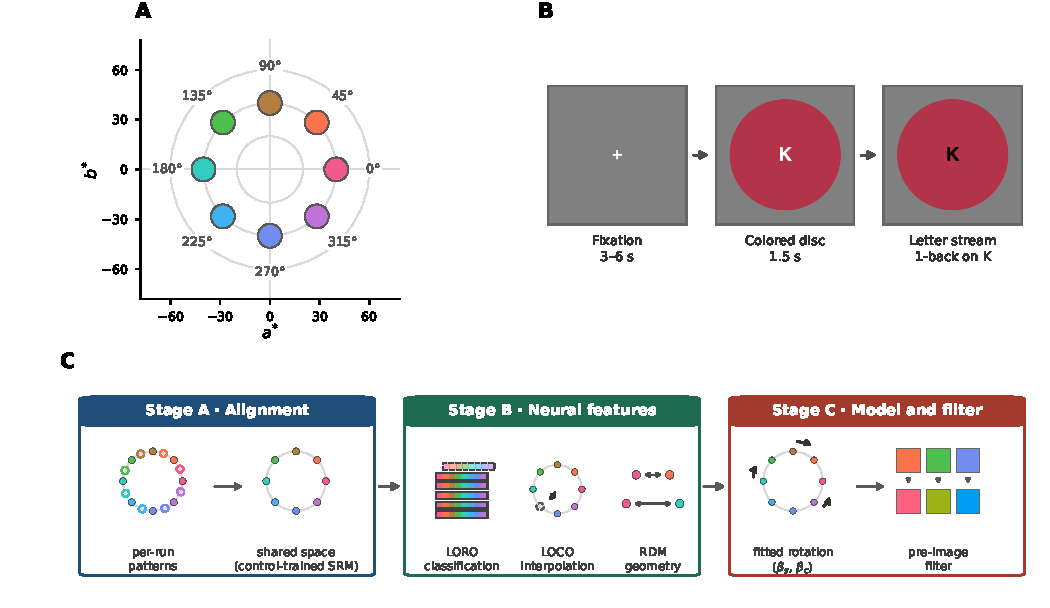
\includegraphics[width=\textwidth]{fig1_paradigm_v3}
  \caption{\textbf{Stimuli, task, and analysis pipeline.} \textbf{(A)} Stimulus set: 8 CIE $L^{*}a^{*}b^{*}$ hues at matched lightness, 45\degree\ angular spacing ($L^{*} = 75$, chroma $= 40$; red--magenta), shown in the $a^{*}b^{*}$ plane. Swatch colors throughout the figure reproduce the displayed stimuli.
  \textbf{(B)} Task: rapid serial visual presentation (RSVP). A fixation period (randomized 3--6\,s) is followed by a 1.5\,s uniform colored disc; 5--9 trials per hue per run (Neurodesign-optimized allocation, identical across participants), six runs.
  \textbf{(C)} Analysis pipeline.
  Stage A (Alignment): two-stage GLM per-hue amplitudes, Procrustes-aligned across runs (open circles, the individual runs before alignment), then projected into a shared response model (SRM) space trained on the $n = 7$ control participants only.
  Stage B (Neural feature): leave-one-run-out (LORO) hue classification, leave-one-color-out (LOCO) hue interpolation, and the representational dissimilarity matrix (RDM) of pairwise distances in that shared space.
  Stage C (Modeling \& filter): a 2-component cortical model whose S-cone-axis ($\beta_s$) and confusion-axis ($\beta_c$) components define the fitted hue rotation; inverting that rotation gives the per-subject stimulus-space filter, which maps each displayed hue to its filtered counterpart.}
  \label{fig:paradigm}
\end{figure}

% ──────────────────────────────────────────────────────────────────────────────
\subsection{Participants}
\label{sec:methods:participants}
% ──────────────────────────────────────────────────────────────────────────────

Ten volunteers provided written informed consent and were enrolled. An additional three respondents were excluded during pre-consent screening because they did not meet MRI safety criteria. The study was approved by the Seoul National University Institutional Review Board (SNUIRB No.~2510/002-023) and conducted in accordance with the Declaration of Helsinki. All participants reported normal or corrected-to-normal visual acuity. Color vision was screened with the 14-plate Ishihara pseudoisochromatic test \parencite{ishihara1917}. Participants who identified 9 or more plates correctly were classified as color-normal controls ($n = 7$, 3 female, aged 20--27 years, mean $22.7 \pm 2.5$). Participants scoring below this threshold were classified as CVD. The classification plates of the same test distinguished the protan from the deutan subtype and indicated anomalous trichromacy rather than dichromacy in both. Two CVD participants completed both sessions, both male. The deutan participant was 24 years old and identified 5 of 14 plates correctly. The protan participant was 25 years old and identified 7 of 14 plates correctly. One further enrolled CVD participant completed the first session but became unavailable before the filter-evaluation session and was excluded from all analyses, leaving nine participants in the analyses. All CVD results are reported as single-case comparisons against the control distribution with the \textcite{crawford1998} modified $t$-test. No population-level inference is made.

% ──────────────────────────────────────────────────────────────────────────────
\subsection{fMRI stimuli and task}
\label{sec:methods:stimuli}
% ──────────────────────────────────────────────────────────────────────────────

Eight chromatic stimuli were defined in CIE $L^{*}a^{*}b^{*}$ space at equal angular spacing in the $a^{*}b^{*}$ plane, from $0^\circ$ to $315^\circ$ in $45^\circ$ steps \parencite{cie1986}. All eight shared a lightness of $L^{*} = 75$ and a chroma of $40$, and they spanned red, orange, yellow, green, cyan, blue, purple, and magenta (Figure~\ref{fig:paradigm}A). A gray filler at the same lightness with $a^{*} = b^{*} = 0$ served as a null condition. Isoluminance was not determined for individual participants. Stimuli were presented on a BOLDscreen 32 UHD monitor (Cambridge Research Systems) at $3840 \times 2160$ resolution, using the Apple XDR Display color preset. The same display and preset served every participant and both sessions.

Stimuli were presented in a rapid serial visual presentation (RSVP) design to sustain attention and fixation. Each trial displayed one uniform chromatic disc, 500 pixels in diameter, for 1.5\,s in a pseudo-random order optimized with Neurodesign \parencite{durnez2018}. Two letters were presented sequentially at the center of the disc, and participants pressed a key on an MRI-compatible button box whenever the letter K appeared twice consecutively. Inter-stimulus intervals were randomly drawn from $\{3, 4.5, 6\}$\,s. Each run comprised 72 events and lasted approximately 7\,min, and each session comprised six runs. The experiment was implemented in PsychoPy 2022.2.5 \parencite{peirce2019}.

The schedule was optimized for detection power rather than for equal counts, so hue counts varied within a run. Each chromatic stimulus occurred 5--9 times per run and 38--47 times across the six runs, and the remaining 14--20 events per run presented the gray filler. Every participant received the same optimized schedule, so this allocation contributes a common component to all individual estimates. All analyses below use a single amplitude per hue and run rather than individual trials, so the varying counts do not enter them.

% ──────────────────────────────────────────────────────────────────────────────
\subsection{Psychophysical tasks}
\label{sec:methods:psychophysical}
% ──────────────────────────────────────────────────────────────────────────────

All participants completed two psychophysical tasks on the day of their first scanning session. The first task measured just-noticeable differences (JNDs) in hue discrimination, and the second was an eight-alternative forced-choice (8AFC) hue-identification task. Both CVD participants repeated both tasks under each filter in the second session (\S\ref{sec:methods:filter_eval}). Both tasks ran outside the scanner under normal room lighting, on a built-in Liquid Retina XDR display set to the same Apple XDR Display color preset.

\paragraph{Just-noticeable difference (JND).}
On each trial two chromatic discs appeared simultaneously to the left and right of fixation, and participants judged whether the two were the same or different. Each disc had a radius of 96 pixels in a $1024 \times 768$ window, their centers were separated by 260 pixels, and their positions were randomized across trials. A fixation cross preceded each trial for 0.5\,s, and the discs remained on screen until the participant responded. The two hues were separated by a fraction $t$ of the pair's full separation, interpolated in CIE $LCh$, and $t$ served as the level of two interleaved 1-up/1-down staircases converging on the level that yields $50\%$ ``different'' responses~\parencite{levitt1971}. The threshold was the mean of the last six reversal levels. Because the two discs always differed, no same trials were included, and the threshold may therefore reflect response bias as well as perceptual sensitivity. Starting levels, step sizes, and termination rules are given in Supplementary~\cref{app:jnd_baseline}.

Eight hue pairs were selected to span the S-cone axis and each subtype's confusion axis. Yellow--purple lies along the S-cone axis, and blue--purple and red--orange are positioned on either side of it. Orange--yellow and yellow--green bracket the deutan confusion axis, and green--blue and cyan--magenta bracket the protan confusion axis. Red--cyan, separated by $180^\circ$, served as a control against ceiling effects. Pair selection was fixed on these grounds before any threshold was collected. For each pair we computed the JND ratio $\gamma = \gamma_{\rm CVD} / \bar{\gamma}_{\rm ctrl}$, in which $\bar{\gamma}_{\rm ctrl}$ denotes the control mean threshold. Ratios above 1 indicate elevated hue-discrimination difficulty relative to controls. Because all participants were measured on the same display, the ratio is unaffected by any difference between that display and the one used in the scanner.

\paragraph{8AFC hue identification.}
Each trial began with a 1.0\,s fixation, followed by a uniform chromatic disc of 500 pixels in diameter for 1.5\,s and a 0.5\,s blank interval. Participants then used the arrow keys to navigate a two-by-four grid of the eight scanner stimulus hues and selected the hue that had been presented. The positions of the eight options were reshuffled on every trial. Trials timed out after 10s without a response. No feedback was provided. Each run comprised 64 trials, eight per hue, in random order. 

% ──────────────────────────────────────────────────────────────────────────────
\subsection{MRI acquisition and preprocessing}
\label{sec:methods:mri}
% ──────────────────────────────────────────────────────────────────────────────

Imaging was performed on a Siemens 3T MAGNETOM Cima.X scanner with a 64-channel head coil. A whole-brain T1-weighted MPRAGE volume served as the anatomical reference. It was acquired sagittally at 1\,mm isotropic resolution, with a repetition time of 2000\,ms, an echo time of 2.36\,ms, a field of view of 256\,mm, a bandwidth of 220\,Hz per pixel, and GRAPPA acceleration factor 2. Functional coverage was restricted to posterior occipital cortex with 24 interleaved oblique slices aligned perpendicular to the calcarine sulcus \parencite{brouwer2009}, spanning 48\,mm. The functional sequence used a repetition time of 1.5\,s, an echo time of 30\,ms, a flip angle of $70^\circ$, and 2\,mm isotropic voxels over a 192\,mm field of view on a $96 \times 80$ matrix. Acceleration was GRAPPA factor 2 without multiband, the bandwidth was 1447\,Hz per pixel, and phase encoding ran right to left. Each run yielded 288--292 volumes. A gradient-echo field map with echo times of 3.88 and 6.34\,ms was acquired in each session and associated with the functional runs in the BIDS metadata.

Data from the first session were converted to BIDS format with the ezBIDS web service \parencite{levitas2024}, accessed in October 2025, which also defaced the anatomical image. The second session was converted with dcm2bids 3.2.0 \parencite{dcm2bids}, and its anatomical image was defaced with Quickshear \parencite{schimke2011}, the same defacing algorithm employed by ezBIDS. Both routes used \texttt{dcm2niix} for DICOM conversion. Preprocessing followed a custom pipeline rather than a standard container, and Supplementary~\cref{app:uncorrected} records the routes that were evaluated and rejected before it was adopted. All steps used FSL 6.0.5.1 and FreeSurfer 7.2.0. The T1w image was skull-stripped with FSL \texttt{bet2} \parencite{smith2002}, and functional images were registered to it by mutual-information coregistration \parencite{wells1996, maes1997}, initialized from the scanner header (FreeSurfer \texttt{mri\_coreg} with \texttt{--regheader}). Normalization to the ICBM 152 Nonlinear Asymmetric 2009c template (MNI152NLin2009cAsym) used a twelve-parameter affine transform (FLIRT) followed by nonlinear warping (FNIRT) \parencite{jenkinson2002, andersson2007}, yielding 2\,mm isotropic BOLD data in MNI space. Each functional volume was resampled once by this composed transform, without slice-timing correction, head-motion correction, susceptibility distortion correction, or spatial smoothing. Because a single transform served every volume in a run, the same spatial interpolation applied throughout. Head-motion correction composes a volume-specific rigid term with that transform. Because volume-specific motion correction introduces additional spatial interpolation that may affect multivoxel patterns \parencite{grootoonk2000}, all neural endpoints were evaluated under both preprocessing schemes. The second pipeline estimated each volume's rigid term with MCFLIRT \parencite{jenkinson2002} and composed it with the normalization transform before the single resampling. The head-motion quality-control record appears in Supplementary~\cref{app:uncorrected}.

% ──────────────────────────────────────────────────────────────────────────────
\subsection{ROI definition and response estimation}
\label{sec:methods:roi}
% ──────────────────────────────────────────────────────────────────────────────

Bilateral V1, V2, V3, and hV4 were defined from the probabilistic atlas of visual topography of \textcite{wang2015}, resampled to 2\,mm and thresholded at a probability above $50\%$. V1, V2, and V3 each merge the ventral and dorsal subdivisions of the atlas. The threshold was applied to each ROI independently, so a voxel assigned to more than one ROI was retained in each. Each ROI was then intersected with that participant's BOLD brain mask, and the resulting coverage is reported in Supplementary~\cref{app:roi_coverage}. Mean voxel counts across the nine analyzed participants were 665 for V1, 458 for V2, 105 for V3, and 64 for hV4, with standard deviations of 209, 113, 19, and 18.

Response amplitudes were estimated with a two-stage general linear model \parencite{dale1999, brouwer2009, brouwer2013}. In the first stage a finite impulse response model with eight delays, spanning 0 to 10.5\,s, was fitted to the concatenated runs without drift terms. Averaging the fitted responses over voxels and over the eight hues gave one hemodynamic response function per ROI and participant.

In the second stage that function and its temporal derivative were convolved with per-hue event sequences and fitted to each run separately by ordinary least squares, alongside a linear and a constant drift term for that run. The result was one amplitude for every voxel, hue, and run, arranged as a $6 \times 8 \times V$ array per participant.

Amplitudes were aligned across runs by a within-subject Procrustes rotation \parencite{gower1975}. For each of runs 2 to 6, the $8 \times 8$ orthogonal matrix $Q_r$ minimizing $\|X_1 - Q_r X_r\|_F$ was applied to that run's hue-by-voxel matrix $X_r \in \mathbb{R}^{8 \times V}$, where $X_1$ is run 1. Scaling was not permitted, so the rotation acts within the eight-dimensional space of hue responses and leaves each voxel's identity unchanged.

% ──────────────────────────────────────────────────────────────────────────────
\subsection{Shared Response Model}
\label{sec:methods:srm}
% ──────────────────────────────────────────────────────────────────────────────

Cross-subject alignment and dimensionality reduction were performed with the Shared Response Model (SRM; \citealp{chen2015}). SRM estimates per-participant orthonormal mappings $W^{\mathrm{srm}}_i \in \mathbb{R}^{V \times k}$ ($V$ voxels, $k$ latent dimensions) and a group-shared response matrix $S \in \mathbb{R}^{k \times 8}$:

\begin{equation}
  \min_{W^{\mathrm{srm}}_i,\,S}\;\sum_{i=1}^N \|X_i - W^{\mathrm{srm}}_i S\|_F^2 \quad\text{s.t.}\quad {W^{\mathrm{srm}}_i}^\top W^{\mathrm{srm}}_i = I_k
\end{equation}

The orthonormality constraint makes the mapping from the shared space back into each participant's voxel space an isometry. Distances and angles in the shared space are therefore those of the reconstructed hue patterns. SRM was trained exclusively on the seven control participants to avoid circular inference in CVD comparisons. Each CVD participant was subsequently projected into the fixed control-derived space by solving $W^{\mathrm{srm}}_\text{CVD} = UV^\top$ where $U\Sigma V^\top = \text{SVD}(X_\text{CVD}\cdot S^\dagger)$. The latent dimension $k$ was chosen per ROI by seven-fold leave-one-subject-out cross-validation, withholding one control participant from SRM training on each fold. Candidate values from 2 to 6 were ranked on each fold by RDM split-half reliability, cross-subject RDM correlation, and reconstruction error, and the value with the best mean rank was selected (Supplementary~\cref{app:dimensionality}). This procedure yielded $k = 4$ for V1 and V2 and $k = 3$ for V3 and hV4.

% ──────────────────────────────────────────────────────────────────────────────
\subsection{Hue-channel basis model}
\label{sec:methods:encoding}
% ──────────────────────────────────────────────────────────────────────────────

Both classification (LORO) and interpolation (LOCO) used the same hue-channel basis model, the forward encoding model of \textcite{brouwer2009}, with separate estimation procedures for decoding and voxel-response prediction. The model represents each stimulus as a $F = 6$-dimensional channel vector $\mathbf{c}(\theta) = [c_1(\theta), \ldots, c_F(\theta)]^\top$, where $c_k(\theta) = \max\!\bigl(0,\,\cos(\theta - \theta_k)\bigr)^2$ is a half-wave rectified squared cosine tuned to preferred hue $\theta_k$, with preferred hues spaced equally at $60^\circ$. Stacking the eight stimulus channel vectors row-wise gives the channel design matrix $C \in \mathbb{R}^{8 \times F}$. Decoding and encoding optimize different targets and therefore estimate the channel-to-voxel weight matrix $W \in \mathbb{R}^{F \times V}$ differently. Decoding recovers the stimulus hue from voxel responses, so we estimated $W$ by the ordinary least-squares pseudoinverse of $C$, reconstructed channel activations for a held-out voxel pattern $\mathbf{x}$ as $\hat{\mathbf{c}} = W\mathbf{x}$, and read out the hue angle, among all 360 integer angles, whose basis vector correlated most strongly with $\hat{\mathbf{c}}$ (\citealp{brouwer2009}; Figure~\ref{fig:forward}). Eight-way classification assigned that angle to the nearest of the eight stimulus hues, and five alternative decoders are compared in Supplementary~\cref{app:decoders}. Encoding predicts the voxel responses as $\hat{X} = CW$ with $\hat{X} \in \mathbb{R}^{8 \times V}$, so we estimated $W$ by ridge regression under a single penalty $\alpha$ chosen for each fit by generalized cross-validation over the voxels of the ROI~\parencite{golub1979} (Supplementary~\cref{app:gcv}). Regularization is warranted because the few stimuli and the correlated basis channels would otherwise overfit $W$ and degrade prediction of held-out responses~\parencite{kay2008,naselaris2011}, and this ridge prior is isotropic and imposes no spatial structure on the voxels.

% ── Figure 2 ─────────────────────────────────────────────────────────────────
\begin{figure}[!htbp]
  \centering
  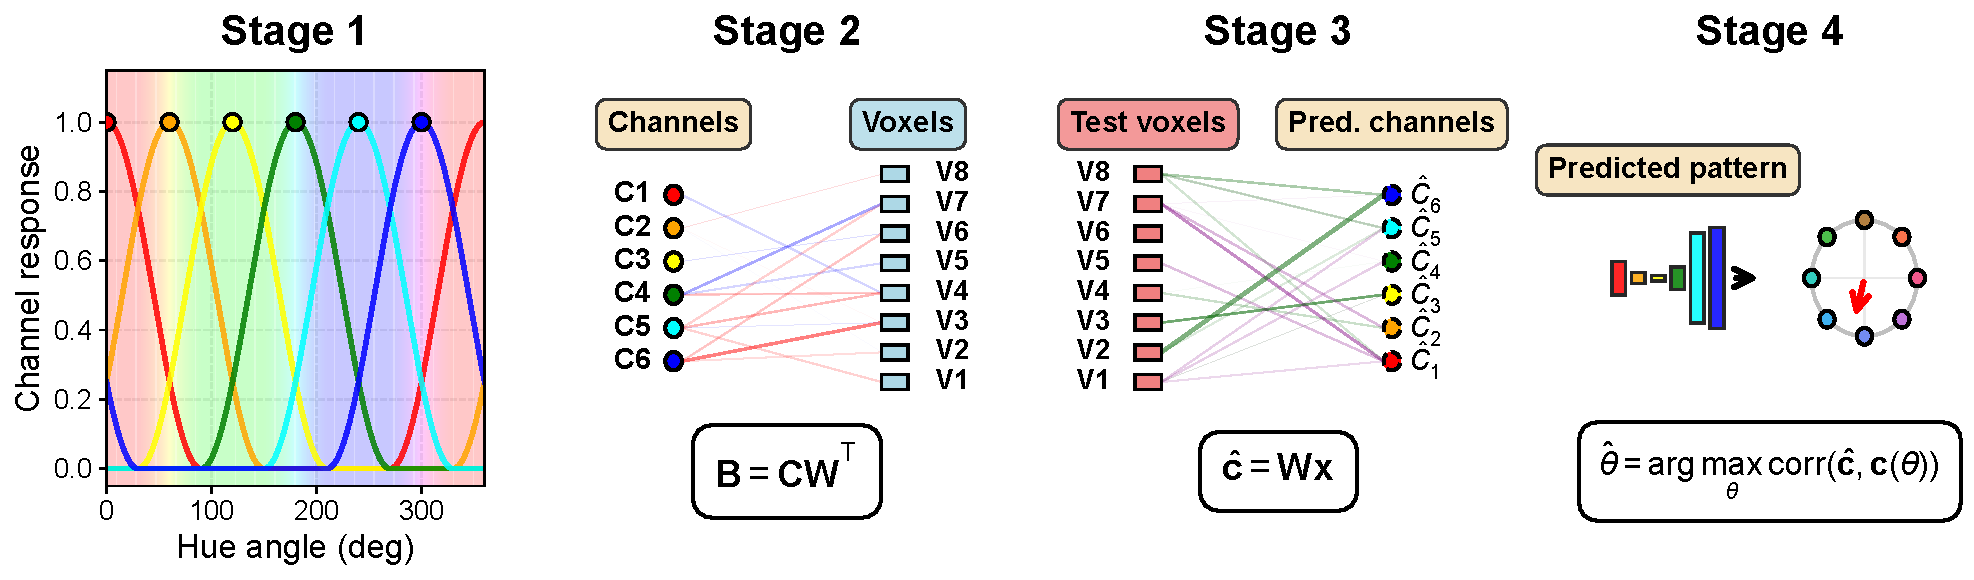
\includegraphics[width=\textwidth]{fig_forward_encoder}
  \caption{\textbf{Hue-channel basis model schematic.}
  Stage 1: each displayed hue is encoded as channel activations by six half-wave rectified squared-cosine basis functions, with preferred hues spaced at 60 degrees \parencite{brouwer2009}.
  Stage 2 (training): the channel-to-voxel weights $W$ are fit by ordinary least squares for hue decoding, or by GCV-regularized ridge regression for voxel-response prediction (encoding).
  Stage 3 (testing): for a held-out voxel pattern, channel activations are reconstructed as $\hat{\mathbf{c}} = W\mathbf{x}$.
  Stage 4: the decoded hue is recovered as the angle, among all 360 integer hues, whose basis vector has the highest Pearson correlation with the reconstructed channel pattern.
  The same model serves both decoding schemes (Section~\ref{sec:methods:loro}): leave-one-run-out classification (LORO) and leave-one-color-out interpolation (LOCO). Their basis and correlation-based selection are identical, and only the held-out test set differs.}
  \label{fig:forward}
\end{figure}

% ──────────────────────────────────────────────────────────────────────────────
\subsection{Two decoding schemes: cross-run classification and cross-color interpolation}
\label{sec:methods:loro}
% ──────────────────────────────────────────────────────────────────────────────

Two cross-validation schemes applied the hue-channel basis model, both computed on the Procrustes-aligned amplitudes of \S\ref{sec:methods:roi}. The leakage control on the run-level alignment, the cross-subject scheme, and the decoding and voxel-prediction metrics are given in Supplementary~\cref{app:cv_metrics}.

\paragraph{Cross-run classification (LORO)}
Hue classification was assessed by leave-one-run-out (LORO) cross-validation, in which every hue remains in the training set, so the scheme tests the categorical representation of the eight hues. For each of the six runs, $W$ was estimated on the remaining five runs from mean-subtracted amplitudes, and the eight hue patterns of the held-out run were decoded by the correlation readout of \S\ref{sec:methods:encoding}. Primary performance was the eight-way classification accuracy averaged across the six folds, against a chance level of $0.125$. Single-case comparisons against the controls are two-tailed here because the hypothesis is preservation, whereas the interpolation tests below are one-tailed (\S\ref{sec:methods:stats}).

Cross-subject transfer of the classifier was evaluated separately, in the SRM-aligned space that makes two participants' voxel spaces correspond (Supplementary~\cref{app:cv_metrics}). Transfer to a held-out control used a leave-one-control-out encoder trained on the remaining six controls, giving 28 participant-by-ROI cells, and transfer to CVD used an encoder trained on all seven controls, giving 8 cells. The two destinations were compared by a Mann--Whitney $U$ test with rank-biserial correlation as the effect size. 

\paragraph{Cross-color interpolation (LOCO)}
\label{sec:methods:loco}
Continuous hue interpolation was assessed by leave-one-color-out (LOCO) cross-validation, in which the held-out hue never appears in training. Each of the eight hues was held out in turn. $W$ was estimated from the remaining seven hues across all six runs, pooled into a 42-sample design matrix, and the held-out hue was predicted by the same correlation readout.

The primary ROI for interpolation was hV4. \textcite{brouwer2009} reconstructed novel hues from V4 and VO1, the ROIs where their interpolation was strongest. LOCO was computed in all four ROIs. Crediting a ROI with interpolation required the control mean to exceed the color-label permutation null defined below. This criterion tests specificity to hue identity rather than overall decodability and identifies the ROIs in which a CVD reduction can be meaningfully interpreted. Single-case CVD comparisons are reported for ROIs meeting the criterion. Values for all four ROIs are given in the Results.

\subparagraph{Adjacent accuracy}
The primary cross-color decoding metric was adjacent accuracy, the proportion of predictions falling within $45^\circ$ of the target hue. This tolerance corresponds to one hue step. Values were averaged across the six runs of each test hue and range from 0 to 1. The readout selects among all 360 integer hues, so a prediction drawn uniformly from that output space falls within tolerance on 91 of 360 draws, giving a chance level of $0.25$. Exact accuracy, which requires the prediction to fall in the correct one of eight $45^\circ$ bins, has a chance level of $0.125$. Control performance was tested against an empirical null of 1,000 random color-label permutations rather than against the analytic chance level. Single-case control--CVD comparisons at hV4 are one-tailed and lower (\S\ref{sec:methods:stats}).

\subparagraph{Vulnerability profile}
The eight-dimensional vector of per-hue adjacent-accuracy values, $\mathbf{v} \in [0,1]^8$, constitutes each participant's \emph{hue vulnerability profile}. Per-hue group comparisons (Figure~\ref{fig:loco}C) are one-tailed and uncorrected (\S\ref{sec:methods:stats}).

% ──────────────────────────────────────────────────────────────────────────────
\subsection{Representational geometry}
\label{sec:methods:rdm}
% ──────────────────────────────────────────────────────────────────────────────

Procrustes disparity measures how far a participant's whole representational geometry lies from the control reference in SRM-aligned space. Disparity was the Procrustes distance between a participant's SRM-aligned $8 \times k$ pattern and that reference. Both patterns were centered on their column means and scaled to unit Frobenius norm. Disparity was then the residual Frobenius norm after the optimal $k \times k$ orthogonal rotation.

The control disparity distribution was estimated by a leave-one-control-out procedure, in which each control participant is compared to the mean of the remaining six, and individual CVD disparity was compared to that distribution one-tailed upper at $\alpha = 0.05$ (\S\ref{sec:methods:stats}). Two estimates of the distribution were computed. The first uses the common control-trained space that every other stage of the pipeline operates in, and the second a symmetric leave-one-subject-out space that projects the held-out control on the same terms as each CVD participant. We report both and treat the symmetric estimate as the inferential test (Supplementary~\cref{app:loo_disparity}; \cref{tab:disparity_loso}). Disparity was additionally recomputed with two distances that use no shared response model, which establishes that it tracks a property of the data rather than of the alignment procedure (Supplementary~\cref{app:triangulation}).
 Because both patterns are scaled to unit norm before the rotation, disparity is insensitive to any difference in overall response magnitude, which is examined separately (Supplementary~\cref{app:activation}).

% ──────────────────────────────────────────────────────────────────────────────
\subsection{Cortical distortion model}
\label{sec:methods:candidates}
% ──────────────────────────────────────────────────────────────────────────────

The distortion model parameterizes the angular displacement $\delta\theta(\theta)$ that maps the displayed hue angle $\theta$ to the angle perceived by a CVD observer. For comparison, a retinal-family model (retinal-plus-gain, R+C) was evaluated on the same criterion and is defined in Supplementary~\cref{app:retinal_family}.

% ── Pipeline schematic — inverse-problem workflow ────────────────────────────
\begin{figure}[htbp]
  \centering
  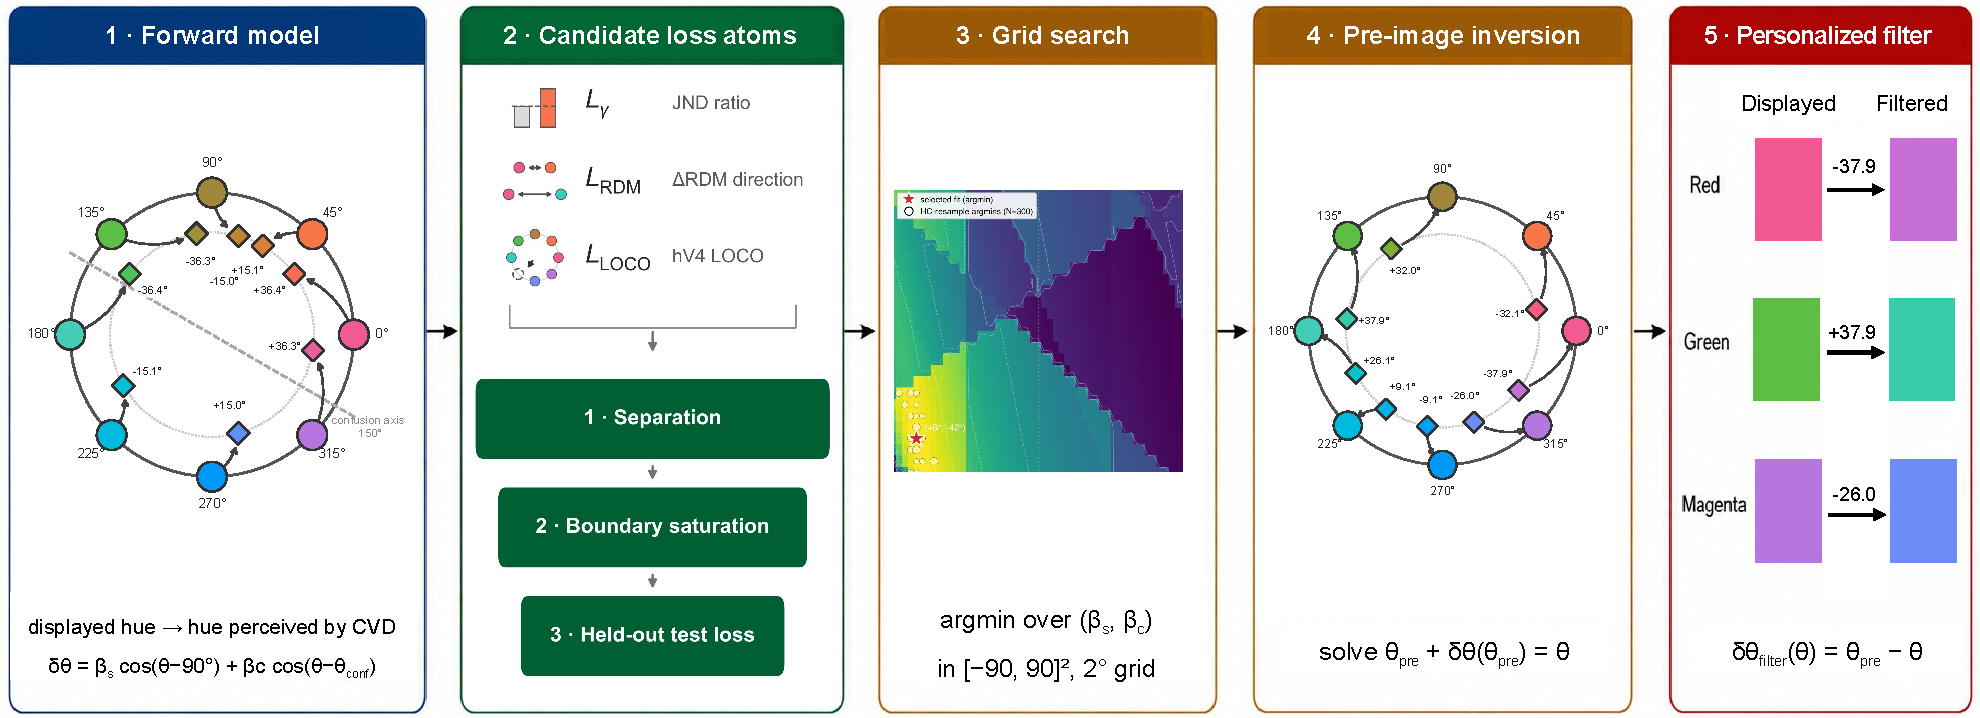
\includegraphics[width=\textwidth]{fig3_workflow}
  \caption{\textbf{Fitting a per-subject cortical distortion and inverting it into a stimulus-space filter.}
  \textbf{(1)} A two-parameter forward model expresses the per-hue distortion as $\delta\theta(\theta) = \beta_s\cos(\theta - 90^\circ) + \beta_c\cos(\theta - \theta_{\rm conf})$: an S-cone-axis component ($\beta_s$) plus a family-specific confusion-axis rotation ($\beta_c$; $\theta_{\rm conf} = 16^\circ$ protan, $150^\circ$ deutan). Outer ring, displayed hue; inner ring, hue perceived under the fitted distortion; labels give the signed displacement.
  \textbf{(2)} Three candidate loss atoms quantify CVD--control differences: the behavioral JND loss ($L_\gamma$), the representational $\Delta$RDM direction ($L_{\rm RDM}$), and hV4 LOCO voxel prediction ($L_{\rm LOCO}$). Combinations of these atoms pass in turn through three gates, on separation, on boundary saturation, and on held-out test loss over $N = 300$ control resamples (\S\ref{sec:methods:selection}).
  \textbf{(3)} A grid search over $\beta_s \in [0^\circ, 50^\circ]$ and $\beta_c \in [-50^\circ, 50^\circ]$ at $2^\circ$ resolution minimizes the $z$-scored composite to the selected fit $\hat\beta$. The surface shown is the deutan participant's; both landscapes and their resample uncertainty are shown in Supplementary~\cref{app:identifiability}.
  \textbf{(4)} The fitted forward map is numerically inverted: for each displayed hue $\theta$, the corrected stimulus $\theta_{\rm pre}$ solves $\theta_{\rm pre} + \delta\theta(\theta_{\rm pre}) = \theta$.
  \textbf{(5)} The individualized filter is $\delta\theta_{\rm filter}(\theta) = \theta_{\rm pre} - \theta$; three of the eight hues are shown for the deutan participant, and the full eight-hue filter for both participants is in Figure~\ref{fig:filter}.
  Hue wheels and swatches are computed from each participant's fitted parameters.}
  \label{fig:pipeline}
\end{figure}

The second model parameterizes the distortion as a sum of two cosine components, one on the S-cone axis and one on each subtype's confusion axis:
%
\begin{equation}
  \delta\theta(\theta;\,\beta_s,\beta_c)
    = \beta_s\cos(\theta - 90^\circ)
    + \beta_c\cos(\theta - \theta_{\rm conf})
  \label{eq:2comp}
\end{equation}
%
where $\theta_{\rm conf}$ is the hue angle assigned to each subtype's confusion direction, $16^\circ$ for protan and $150^\circ$ for deutan. Both angles are fixed before fitting. They are defined in a cone-opponent convention and applied to the nominal $L^{*}a^{*}b^{*}$ hue angle of the stimuli, which is an approximation we adopt for the whole model. $\beta_s$ parameterizes distortion along the S-cone axis ($\theta = 90^\circ$) and $\beta_c$ along the individual confusion axis. Each component has a fixed direction and a free amplitude, so the model spans distortions in the plane defined by those two axes. The parameters were bounded before fitting at $\beta_s \in [0^\circ, 50^\circ]$ and $\beta_c \in [-50^\circ, 50^\circ]$. The non-negative bound on $\beta_s$ is an assumption of the model rather than a biologically grounded mechanism. Model adequacy was assessed by the procedure in \S\ref{sec:methods:selection}; results are reported in \S\ref{sec:results:twocomp}.

% ──────────────────────────────────────────────────────────────────────────────
\subsection{Inverse fitting}
\label{sec:methods:twocomp}
% ──────────────────────────────────────────────────────────────────────────────

Per-subject distortion parameters $(\beta_s,\beta_c)$ were estimated by finding the distortion that, when applied to control-derived neural representations, best reproduces the observed CVD responses. Three loss families served as the fitting objective, and a specific instance of a family is a \emph{loss atom}.

\paragraph{Psychophysical JND loss ($L_\gamma$).}
A distortion changes the perceived angular separation of a hue pair, and a pair that is compressed becomes harder to discriminate. We modeled the predicted threshold for a pair as $\hat{\gamma} = \bar{\gamma}_{\rm ctrl}\,(d_{\rm phys} / d_{\rm perc})$, where $d_{\rm phys}$ is the separation of the two hues on the display, $d_{\rm perc}$ is their separation after the candidate distortion of Eq.\,\ref{eq:2comp}, and $\bar{\gamma}_{\rm ctrl}$ is the control mean threshold for that pair. The loss is the squared difference between the predicted and the observed CVD threshold, standardized by the control standard deviation $s_{\rm ctrl}$ for that pair and summed over the pairs entering the atom:
%
\begin{equation}
  L_\gamma = \sum_{p}\left(\frac{\hat{\gamma}_p - \gamma_{{\rm CVD},p}}{s_{{\rm ctrl},p}}\right)^{\!2}
  \label{eq:lgamma}
\end{equation}
%
The atoms available to the fitting were single-pair terms and one aggregate term. The single-pair candidates were the pairs that bracket each participant's confusion axis and the S-cone pair (\S\ref{sec:methods:psychophysical}), namely orange--yellow, yellow--green, and yellow--purple for the deutan participant and green--blue for the protan participant. The aggregate term $\gamma_{\rm all}$ sums over all eight tested pairs.

\paragraph{Per-pair RDM difference ($\Delta$RDM).}
The optimal rotation in Procrustes disparity (\S\ref{sec:methods:rdm}) removes the information about which hues are displaced. Inverting the distortion requires that information. We therefore expressed the same comparison as a difference of representational dissimilarity matrices \parencite{kriegeskorte2008}, which retains the displacement of every hue pair. For each participant and ROI the RDM was the $8 \times 8$ matrix of pairwise correlation distances ($1 - \text{Pearson}\,r$) among the reduced hue patterns of that ROI, and the per-pair difference was $\Delta\text{RDM} = \text{RDM}_\text{CVD} - \overline{\text{RDM}}_\text{ctrl}$, in which $\overline{\text{RDM}}_\text{ctrl}$ is the mean RDM over the seven control participants.

\paragraph{Representational $\Delta$RDM loss ($L_{\rm RDM}$).}
For a candidate distortion, a simulated difference $\Delta\text{RDM}_{\rm sim}$ is obtained by applying $\delta\theta$ to the control mean RDM and comparing it to the observed $\Delta\text{RDM}$. Each distorted hue is assigned to the nearest of the eight $45^\circ$ bins, so $\Delta\text{RDM}_{\rm sim}$ is built by reindexing the entries of the control mean RDM. A candidate distortion therefore acts as a permutation of the eight hues, and distortions that map to the same permutation are indistinguishable to this term. The loss is the cosine dissimilarity between the observed and simulated 28-element upper-triangle vectors:
%
\begin{equation}
  L_{\rm RDM} = 1 - \cos\!\bigl(\Delta\text{RDM}_{\rm sim},\,
    \Delta\text{RDM}_{\rm obs}\bigr)
  \label{eq:lrdm}
\end{equation}
%
Because the loss is a cosine, the magnitude of $\Delta$RDM does not enter.

The loss computes $\Delta$RDM in a PCA-reduced space ($K = 6$). Across the 28 pairwise entries this estimate agreed with the SRM-aligned estimate used for disparity at V1, V2 and hV4 ($r = 0.77$--$0.89$), and less closely at V3 ($r = 0.39$--$0.58$), so the reduction does not determine the pattern the loss fits. The PCA basis is the production basis. The full selection and fitting procedure was additionally repeated with the RDM atoms computed in the SRM-aligned space, and the agreement between the two reductions is reported with the fits (\S\ref{sec:results:twocomp}, Supplementary~\cref{app:identifiability}).

\paragraph{Composite loss and grid search.}
A third atom, $L_{\rm LOCO}$, scored how well a candidate distortion accounted for the CVD participant's own held-out responses at hV4. It was available to every candidate objective, is defined in Supplementary~\cref{app:identifiability}, and the selection procedure admitted it in neither participant. The atoms differ in scale, so each was evaluated over the full parameter grid and standardized to zero mean and unit standard deviation across that grid, which leaves the composite invariant to rescaling an individual atom by a positive constant. The composite loss is the sum of the standardized atoms divided by $\sqrt{n_a}$, where $n_a$ is the number of atoms.

The grid was exhaustive at $2^\circ$ resolution, with $\beta_s$ over $[0^\circ, 50^\circ]$ (26 values) and $\beta_c$ over $[-50^\circ, 50^\circ]$ (51 values), giving $1{,}326$ cells, and for the R+C comparison model (Supplementary~\cref{app:retinal_family}) $g$ was searched over $[0, 3]$ in steps of $0.05$ (61 values).

% ──────────────────────────────────────────────────────────────────────────────
\subsection{Parameter selection}
\label{sec:methods:selection}
% ──────────────────────────────────────────────────────────────────────────────

Per-subject loss combinations and model class were selected by a pre-specified three-gate procedure, with inputs from two resampling schemes over the seven control references, a 5-train/2-test resample repeated $N = 300$ times and a strict 7-fold leave-one-control-out, both using the same loss atoms. Gate 1 set a separation precondition, admitting an atom only when its CVD loss value differed from the control leave-one-out distribution by a Cohen's $d$ of magnitude $0.5$ or greater in either direction. Gate 2 rejected admitted combinations in which at least half of the resample solutions saturated the grid boundary, since boundary saturation indicates model misspecification. It also rejected combinations whose recovered parameters collapsed across resamples, defined as an interquartile range above $50^\circ$ or a sign reversal between the training and test argmin exceeding $5^\circ$. Gate 3 ranked the surviving combinations by the median composite test-loss $\overline{L}_{\rm test}$ over the $N = 300$ resamples, evaluated for each resample at the training argmin on the two held-out controls and z-normalized relative to the training grid, so that a lower value indicates generalization to unseen control references. Ties were broken by the test-loss interquartile range, which measures the stability of that generalization estimate, and these two quantities were the only ranking criteria. Because admission and ranking use effect size and held-out test loss, the fitted parameters do not depend on whether any single disparity contrast reaches significance.

Further quantities were recorded for each candidate outside the ranking. The held-out neural loss $\overline{L}_{\rm RDM}^{\rm LOO}$ from the strict 7-fold leave-one-out evaluates a candidate's neural atoms with the psychophysical term excluded. It therefore isolates what the neural terms alone contribute to the fit. Parameter stability was summarized by the interquartile range of the recovered $(\hat\beta_s, \hat\beta_c)$, by the fraction of resamples recovering the modal $45^\circ$ bin, and by the strict 7-fold parameter range. The control false-positive rate and the distribution of fitted parameter magnitudes over the same control refits are likewise reported descriptively in Supplementary~\cref{app:identifiability} and \cref{app:fit_stability}. To attribute the fit between the two loss families, each selected objective was additionally refit with the psychophysical atom alone, with the neural atom alone, and with the RDM atom removed. These ablation are reported descriptively in \S\ref{sec:results:neural_role}.

% ──────────────────────────────────────────────────────────────────────────────
\subsection{Identifiability and recovery}
\label{sec:methods:identifiability}
% ──────────────────────────────────────────────────────────────────────────────

Four pre-specified checks were run on the loss combination selected for each participant in \S\ref{sec:methods:selection}. The checks bound what the fit can estimate and entered no selection decision. Test~1 asks whether a known distortion can be recovered at the present sample size and noise level. Synthetic CVD responses were generated at a known ground truth by passing that distortion through each control participant's encoder, with noise matched to that participant's residual structure, and the grid fit was re-run on each synthetic dataset. The refit repeats the grid search rather than the full selection procedure, so it measures recoverability at a fixed loss combination. Test~2a repeats the same synthesis with ground truth at $(0^\circ, 0^\circ)$ and each control participant's real thresholds, so the spread of its refits sets the per-axis uncertainty floor. Test~2b refits each of the seven control participants as a pseudo-CVD case, with the remaining controls as the reference pool, and places the CVD estimate among the seven control estimates by a one-sided rank-distance percentile. Test~2c permutes the eight color labels of the real CVD amplitudes $N = 1000$ times, asking whether the estimate depends on which hue evoked which response. Tests~1, 2b and 2c across the two production candidates gave six tests, corrected together under the Benjamini--Hochberg false-discovery rate ($\alpha = 0.05$). Outcomes are summarized in \S\ref{sec:results:twocomp} and reported in full in Supplementary~\cref{app:identifiability}.

% ──────────────────────────────────────────────────────────────────────────────
\subsection{Stimulus-space filter and its evaluation}
\label{sec:methods:filter}
\label{sec:methods:filter_eval}
% ──────────────────────────────────────────────────────────────────────────────

The correction filter for each participant is the pre-image of the fitted transform $T(\hat{\beta}_s, \hat{\beta}_c): \theta \mapsto \theta + \delta\theta(\theta;\hat{\beta}_s,\hat{\beta}_c)$. For each of the eight displayed hues $\theta_k$ we solved $T(\tilde{\theta}_k) = \theta_k$ for the input angle $\tilde{\theta}_k$, which gives a per-hue correction $\delta\theta_k^{\rm filt} = \tilde{\theta}_k - \theta_k$. All eight hues resolved to within $10^{-3}$ degrees of their target in both participants, and the procedure rejects a parameter set that leaves any hue unresolved. We assume that, under the fitted model, a CVD observer viewing $\tilde{\theta}_k$ obtains the cortical hue representation that a control observer obtains when viewing $\theta_k$.

Both CVD participants completed a second scanning session under two filters, their individualized filter and a deployed macOS accessibility filter, each compared against the unfiltered Session-1 baseline. The individualized filter used the parameters selected in \S\ref{sec:methods:selection}. Acquisition, comparator, run count, condition order, and single-case-inference details are given in Supplementary~\cref{app:filter_eval}.

Within each condition we recomputed the primary Session-1 interpolation metric (LOCO adjacent accuracy, \S\ref{sec:methods:loco}), LORO classification, SRM Procrustes disparity into the control-derived shared space, and the representational dissimilarity matrices, and we repeated the JND and 8AFC tasks of \S\ref{sec:methods:psychophysical} against both the unfiltered Session-1 baseline and the control distribution. Each neural index is reported as the case-control effect size $d_{cc}$ (\S\ref{sec:methods:stats}), which places that participant's value against the seven-control distribution. No $p$ value is attached, because the grand-mean permutation null is biased for this design, and the cross-session psychophysical comparison is likewise descriptive. Condition-level values for every index appear in Supplementary~\cref{app:exp2_outcomes}.

% ──────────────────────────────────────────────────────────────────────────────
\subsection{Statistical analysis}
\label{sec:methods:stats}
% ──────────────────────────────────────────────────────────────────────────────

Single-case comparisons of a CVD participant against the seven controls used the Crawford--Howell modified $t$ with $df = 6$ \parencite{crawford1998}, one-tailed toward a deficit unless a subsection states otherwise, and are reported with the case-control effect size $d_{cc} = t\sqrt{8/7}$ (Supplementary~\cref{app:statistics}). Control-level interpolation was tested against an empirical null of $1{,}000$ within-participant color-label permutations, and group control--CVD comparisons against $10{,}000$ subject-label permutations \parencite{nichols2002}. Families of related tests were corrected by the Benjamini--Hochberg procedure at $\alpha = 0.05$, applied to the six identifiability tests of \S\ref{sec:methods:identifiability} and to the participant-by-region grids of the supplementary color-correspondence analysis. Identification accuracy carries Wilson score intervals over the $n = 64$ trials of each condition, and group effect sizes are reported as Hedges' $g$.

% ──────────────────────────────────────────────────────────────────────────────
\subsection{Reproducibility}
\label{sec:methods:repro}
% ──────────────────────────────────────────────────────────────────────────────

All analyses were conducted in Python 3.10 with numpy 1.24.3, scipy 1.11.3, scikit-learn 1.3.0 \parencite{pedregosa2011}, and BrainIAK 0.11. Random seeds were fixed for every permutation test and bootstrap, and each script records its own value. Code availability and the access conditions on the neuroimaging data are stated in the Data and Code Availability section.

% Results Section
% Results Section — v4 (2026-05-14)
% Changes from v3:
%   - Figure numbering: Fig 1 (paradigm), Fig 2 (forward encoder),
%                       Fig 3 (LORO/LOCO), Fig 4 (geometry),
%                       Fig 5 (2-component), Fig 6 (filter)
%   - Fig 1 (paradigm) moved to Methods to render before Fig 2 (forward encoder).
%   - Primary model: 2-component throughout; Machado and R+C comparisons moved to Appendix A
%   - LOCO metric updated: adjacent accuracy (adj_acc, 0–1, higher = better)
%     replacing circular correlation rho
%   - Fig 4 (SRM geometry/ΔRDM) added as separate figure
%   - Fig 1 is a PowerPoint-generated schematic: placeholder box below
%   - All captions from FIGURE_CAPTIONS.md (2026-05-11 revision)
% 2026-05-14 update (Option C adoption):
%   - Loss changed HYBRID → Option C (neural-primary 4-term + heavy Tikhonov, Methods Eq. 2).
%     Canonical production argmins (frozen for Phase-3): the deutan participant (+6,-42); the protan participant (+2,+24).
%   - Brettel directional-consistency text removed per 2026-05-14 revalidation.
%   - The deutan participant filter-direction description rewritten for new argmin.
%   - Model-class ceiling caveat added.
%   - HYBRID backup at results_v4_HYBRID_backup.tex.

\section{Results}
\label{sec:results}

% ──────────────────────────────────────────────────────────────────────────────
\subsection{Categorical hue information remains decodable while hue interpolation falls to chance at hV4 in both CVD cases}
\label{sec:results:loro}
\label{sec:results:loco}
% ──────────────────────────────────────────────────────────────────────────────

Under leave-one-run-out (LORO) cross-validation both CVD participants classified all eight hues above the $0.125$ chance level at every ROI (lowest $0.375$ at hV4, three times chance; Figure~\ref{fig:loco}A; \S\ref{sec:methods:loro}). Thus, hue identity remained recoverable from cortical activity, satisfying our prespecified information-preservation criterion for subsequent filter construction. Classification was likewise preserved under head-motion correction, where the lowest CVD cell across the four ROIs was $0.229$, still $1.8$ times chance, and no single-case contrast approached significance in either pipeline (\cref{tab:interp_arms}). Repeating the readout in the SRM-aligned space reproduces the pattern (Supplementary~\cref{app:alignment}). This parallels psychophysical evidence that the perception of large color differences remains largely intact in anomalous trichromacy \parencite{boehm2014}.

An encoder built from the controls also decoded hues from the CVD participants' cortical responses. Accuracy on their held-out runs averaged $0.432$ over the eight participant-by-ROI cells, above the $0.125$ chance level ($t(7) = 6.51$, $p < 0.001$), against $0.526$ over the 28 cells of the held-out controls ($p = 0.052$; Supplementary~\cref{app:decoders}). A channel-to-voxel weight matrix from the controls therefore transfers to CVD cortex. 

Hue interpolation, by contrast, succeeded at hV4 alone in the controls (adjacent accuracy $0.456 \pm 0.039$, mean $\pm$ SEM over $n = 7$; $p = 0.011$ against $1{,}000$ per-subject color-label permutations). Interpolation was measured by leave-one-color-out (LOCO) decoding, for which the analytic chance level is $0.25$ (\S\ref{sec:methods:loco}). All four ROIs exceeded $0.25$, but the permutation null lay near $0.35$ (Supplementary~\cref{app:uncorrected}), and V1 to V3 stayed within it ($0.393$, $0.357$, and $0.339$; $p = 0.164$, $0.424$, $0.586$). The localization held under head-motion correction, with hV4 again above its null ($0.451$, $p = 0.023$) and V1 to V3 within theirs ($0.283$, $0.381$, $0.315$; $p \geq 0.228$; \cref{tab:interp_arms}). This replicates \textcite{brouwer2009} and fixes hV4 as the ROI where a CVD reduction in interpolation is interpretable.

Both CVD participants fell below the control distribution at hV4, significantly so in the protan participant (adjacent accuracy $0.13$; Crawford \& Howell $t = -3.04$, $p = 0.012$, $d_{cc} = -3.25$) and at $d_{cc} = -2.02$ in the deutan participant ($0.25$; $t = -1.89$, $p = 0.054$), against a control mean of $0.46$ (Figure~\ref{fig:loco}B). The magnitude of this reduction was sensitive to preprocessing: under head-motion correction both single-case contrasts returned $p > .10$, and only the primary-pipeline protan contrast excluded zero from its effect-size interval (\cref{tab:interp_arms}). The positions relative to the controls nevertheless stayed consistent, with both participants below the control mean in each pipeline, all seven controls above the protan participant, and at least five above the deutan participant. Categorical identification and continuous interpolation thus dissociate within the same hV4 voxels and runs, a pattern that indicates a deficit specific to hue interpolation rather than a general loss of signal quality.

This reduction concentrated on the S-cone intermediate hues. Both participants gave zero adjacent accuracy at hV4 for blue, purple, and magenta, giving identical single-case statistics ($d_{cc} = -2.06$, $-0.85$, and $-1.57$; Figure~\ref{fig:loco}C). Per-hue tests reached $p \geq 0.051$ at every hue (Crawford \& Howell, one-tailed, uncorrected and exploratory), with blue the largest deviation. The per-hue accuracies form each participant's hue vulnerability profile $\mathbf{v} \in [0,1]^8$.

% ── Figure 3 ─────────────────────────────────────────────────────────────────
\begin{figure}[htbp]
  \centering
  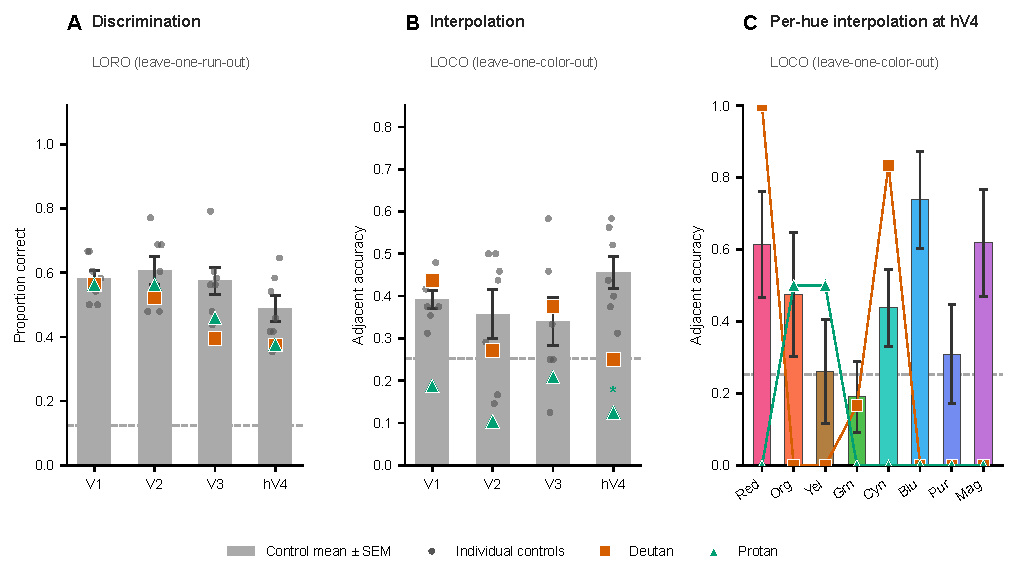
\includegraphics[width=\textwidth]{fig2_loro_loco}
  \caption{\textbf{Hue classification and interpolation across V1--hV4 in the two CVD participants and controls.} All panels are computed on the Procrustes-aligned amplitudes with $n = 7$ controls at every ROI. Gray bars give the control mean $\pm$ SEM, the orange square the deutan participant, and the teal triangle the protan participant.
  \textbf{(A)} Eight-way classification accuracy from leave-one-run-out cross-validation of the hue-channel basis model. The dashed line marks the chance level of $1/8$. Single-case Crawford--Howell comparisons are two-tailed here, since the hypothesis is preservation.
  \textbf{(B)} Adjacent accuracy from leave-one-color-out cross-validation, the proportion of predictions falling within $45^\circ$ of the target hue. The dashed line marks the analytic chance level of $0.25$. Asterisks give one-tailed single-case Crawford--Howell comparisons and appear only at ROIs whose control mean exceeds the color-label permutation null.
  \textbf{(C)} Per-hue adjacent accuracy at hV4. Per-hue comparisons are one-tailed, uncorrected, and exploratory.}
  \label{fig:loco}
\end{figure}

% ──────────────────────────────────────────────────────────────────────────────
\subsection{Hue geometry departs from the control reference in both CVD cases}
\label{sec:results:geometry}
% ──────────────────────────────────────────────────────────────────────────────

Procrustes disparity from the control reference rose in both CVD participants (Figure~\ref{fig:geometry}). The region carrying the largest deviation remained V1 in the protan participant across both pipelines and varied in the deutan participant, at V2 in the primary pipeline and at V1 under head-motion correction. Under the symmetric leave-one-subject-out reference, the protan V1 elevation reached significance in the primary pipeline ($p = .045$) and the remaining cells stayed within the control range. We therefore report the regional attribution as descriptive and treat the disparity structure as the quantity that the neural loss term evaluates (Supplementary~\cref{app:uncorrected}).

Full test statistics and effect sizes for both estimators and both pipelines are reported in \cref{tab:disparity_loso} and \cref{tab:motion_arms}, and the validity checks for the geometric comparison appear in Supplementary~\cref{app:geometry_validity}.

% ── Figure 4 ─────────────────────────────────────────────────────────────────
\begin{figure}[htbp]
  \centering
  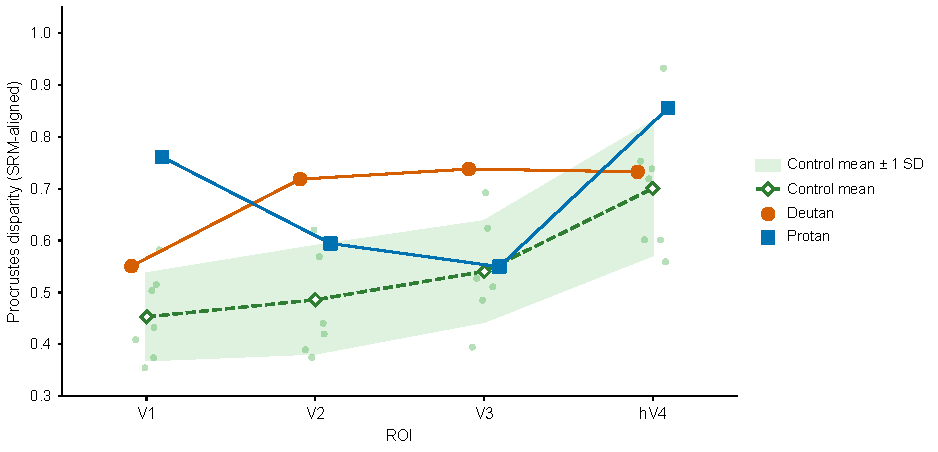
\includegraphics[width=\textwidth]{fig3_geometry_r6}
  \caption{\textbf{Procrustes disparity to the control reference.}
  Disparity per participant and ROI, indexing the distance of the whole hue geometry from that reference.
  The gray band gives the control group mean $\pm 1$ SD ($n = 7$) and the dots give the individual control leave-one-out values.
  Single-case comparisons used the Crawford--Howell modified $t$ against the control leave-one-out distribution, one-tailed.
  Asterisks are omitted; region-wise tests for both preprocessing pipelines and both references are given in Supplementary~\cref{app:uncorrected} and \cref{tab:disparity_loso}.}
  \label{fig:geometry}
\end{figure}

% ──────────────────────────────────────────────────────────────────────────────
\subsection{Hue-discrimination threshold elevations are axis-specific in both participants}
\label{sec:results:jnd}
% ──────────────────────────────────────────────────────────────────────────────

In the just-noticeable-difference (JND) task (\S\ref{sec:methods:psychophysical}), each CVD participant's threshold elevations aligned with the confusion axis of their own subtype. In the deutan participant the two pairs bracketing the deutan axis were elevated, orange--yellow ($\gamma = 3.02$, $z = +4.15$) and yellow--green ($\gamma = 3.10$, $z = +4.32$), as was the S-cone pair yellow--purple ($\gamma = 2.87$, $z = +6.70$). In the protan participant the elevation was confined to green--blue, which brackets the protan axis ($\gamma = 1.95$, $z = +2.36$). Here $\gamma$ is the ratio of the participant's threshold to the control mean and $z$ is the deviation in control standard deviations ($n = 7$).

The remaining pairs lay within the control range in both participants ($|z| \leq 1.23$). This includes red--cyan, the $180^\circ$ control pair, where both participants discriminated more finely than the controls ($\gamma = 0.45$). Mean $|z|$ over the eight pairs was $2.24$ in the deutan and $0.90$ in the protan participant. Values for all eight pairs appear in Supplementary~\cref{app:jnd_baseline}. Discrimination off those axes matches or exceeds the control level, so the elevations mark an axis-specific deficit rather than a general loss of chromatic sensitivity.

% ──────────────────────────────────────────────────────────────────────────────
\subsection{A common cortical model fits both CVD cases}
\label{sec:results:twocomp}
\label{sec:results:rc_insufficient}

The separation precondition determined the candidate grid. The RDM atom entered only at ROIs where it separated the participant from the control distribution (Section~\ref{sec:methods:selection}), which left all four ROIs in the deutan participant and V1 alone in the protan participant (per-ROI separations in \cref{tab:fit_stability}). The psychophysical axis was enumerated in full. Both winning loss combinations paired a JND atom with a $\Delta$RDM atom, and the LOCO family entered neither.

For the deutan participant ($\theta_{\rm conf} = 150^\circ$), $\gamma_{\rm OY} + L_{\rm RDM}^{(V2)}$ ranked first among the 25 combinations passing the boundary-saturation gate and returned $(\hat\beta_s, \hat\beta_c) = (6^\circ, -42^\circ)$, ahead of the $\beta_s$-dominant candidate that also passed. For the protan participant ($\theta_{\rm conf} = 16^\circ$), $\gamma_{\rm all} + L_{\rm RDM}^{(V1)}$ ranked first among four, and every gate-passing combination returned $(2^\circ, +24^\circ)$. Held-out losses and their spread are in \cref{tab:modelfits}.

Both fits generalized to held-out control data. On every leave-one-out fold the fitted distortion predicted the CVD representational geometry more closely than the null distortion $(0^\circ, 0^\circ)$, and on held-out loss each selected cell ranked within the top $8\%$ of the $1{,}326$-cell grid (per-participant percentiles and losses in \cref{tab:fit_stability}).

Each participant's selected fit is the global minimum of its loss surface on the full data. The deutan estimate is robust across the 300 resamples, the seven leave-one-out folds, and both basis reductions, and its confusion-axis magnitude ($42^\circ$) exceeds the $26^\circ$ recovery uncertainty of the procedure. The protan estimate, however, is basis-sensitive, returning $(2^\circ, +24^\circ)$ under the PCA basis but $(32^\circ, 0^\circ)$ under the SRM basis, and its $24^\circ$ magnitude lies within the recovery uncertainty. None of the six pre-specified identifiability tests of parameter recovery, CVD specificity, and color specificity reached significance after Benjamini--Hochberg correction, so the fitted optima are reported as descriptive embeddings of the distortion rather than physiological point estimates. The fitted S-cone amplitudes of $6^\circ$ and $2^\circ$ fall below the recovery uncertainty on that axis in both participants, so that component's magnitude is bounded rather than estimated (Supplementary~\cref{app:identifiability}).

By contrast, the retinal-family comparison model does not represent this distortion. Its single gain rescales the Machado cone shift along the confusion axis alone, cannot express the S-cone displacement on which the interpolation deficit concentrates, and saturated the gain boundary in both participants ($g = 3.0$ and $2.95$). Scored on the same held-out composite, its protan fit reached $\overline{L}_{\rm test} = -0.86$ against $-1.54$ for the 2-component model (Supplementary~\cref{app:retinal_family}).


% ──────────────────────────────────────────────────────────────────────────────
\subsection{The neural term relocates the protan fit and sharpens the deutan fit}
\label{sec:results:neural_role}
% ──────────────────────────────────────────────────────────────────────────────

The neural term moved the fitted optimum in the protan participant and sharpened it in the deutan participant. Without the RDM atom the protan optimum sits at the S-cone-dominant $(26^\circ, +4^\circ)$, and with it at the confusion-axis-dominant $(2^\circ, +24^\circ)$. At that estimate only the RDM term separates from the no-distortion control (\cref{tab:fit_stability}), so the confusion-axis component of the protan distortion is carried by the neural data.

In the deutan participant the RDM atom adds precision rather than direction. The psychophysical atoms alone settle at $(16^\circ, -44^\circ)$, the combined fit at $(6^\circ, -42^\circ)$, and a neural-only fit at $(4^\circ, -26^\circ)$, all on the same side of the confusion axis, and adding the RDM atom more than halved the boundary-saturation rate (\cref{tab:fit_stability}). The neural term therefore sharpens a direction that the psychophysical atoms already fix.

The neural term also narrowed the resample spread in both participants, under both basis reductions (\cref{tab:fit_stability}). In the protan participant the SRM reduction places the optimum at $(32^\circ, 0^\circ)$ rather than at the PCA solution. The neural term therefore contributed information that the psychophysical atoms alone did not carry.
% ──────────────────────────────────────────────────────────────────────────────

% ──────────────────────────────────────────────────────────────────────────────
\subsection{Per-subject stimulus-space filter}
\label{sec:results:filter}
% ──────────────────────────────────────────────────────────────────────────────

Each filter is the exact numerical pre-image of that participant's fitted 2-component transform (Section~\ref{sec:methods:filter}). The mean per-hue correction is $26.3^\circ$ for the deutan participant ($\hat\beta_s = 6^\circ$, $\hat\beta_c = -42^\circ$, $\theta_{\rm conf} = 150^\circ$) and $16.2^\circ$ for the protan participant ($2^\circ$, $+24^\circ$, $16^\circ$), and the per-hue values are drawn in Figure~\ref{fig:filter}. Both filters were frozen on the primary pipeline before the second session and were not re-derived, so the preprocessing comparison leaves the evaluated filter unchanged (Supplementary~\cref{app:fit_stability}).

% ── Figure 7 — per-subject stimulus-space filter (Original | Filtered) ───────
\begin{figure}[!htbp]
  \centering
  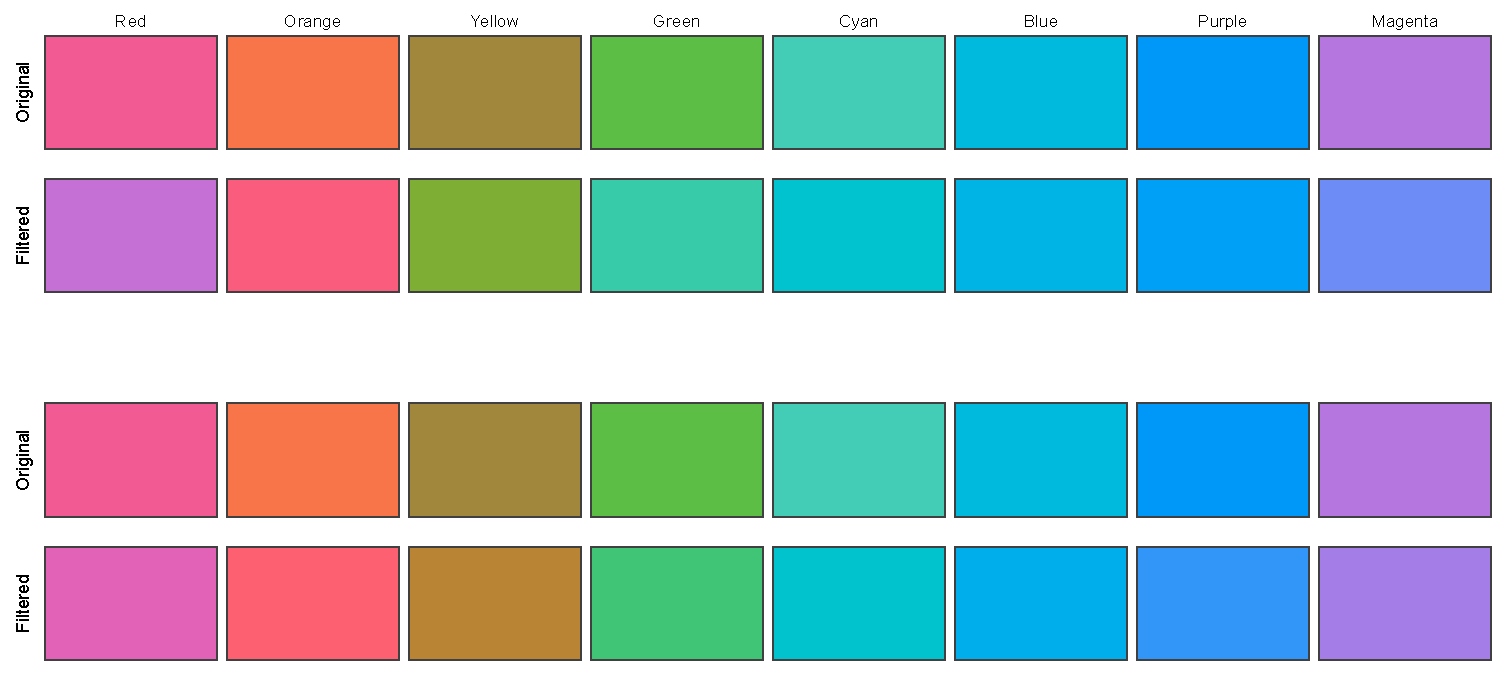
\includegraphics[width=\textwidth]{fig7_filter}
  \caption[Per-subject stimulus-space correction filter]{\textbf{Per-subject stimulus-space correction filter.}
  For each CVD participant, the displayed stimulus (\emph{Original}) and the corrected stimulus (\emph{Filtered}) are shown for the eight scanner hues, which run across the columns.
  Top block: the deutan participant, $(\hat\beta_s, \hat\beta_c) = (6^\circ, -42^\circ)$.
  Bottom block: the protan participant, $(\hat\beta_s, \hat\beta_c) = (2^\circ, +24^\circ)$.
  The filtered stimulus is the exact numerical pre-image of the fitted 2-component transform. The per-hue corrections $\delta\theta_{\rm filter} = \theta_{\rm pre} - \theta$ are reported in Section~\ref{sec:results:filter}, and both filters are evaluated in Section~\ref{sec:results:filter_eval} and \cref{fig:filter_eval}.}
  \label{fig:filter}
\end{figure}

% ──────────────────────────────────────────────────────────────────────────────
\subsection{Psychophysical and neural filter evaluation}
\label{sec:results:filter_eval}
% ──────────────────────────────────────────────────────────────────────────────

\paragraph{Psychophysics.}
In the deutan participant both filters removed the baseline deficit. All three elevated pairs returned to within $\pm 1.8$ control SDs, the mean $|z|$ fell from $2.24$ to below $0.9$ under each filter, and the two filters were indistinguishable on thresholds (Wilcoxon $p = 0.84$).

In the protan participant the two filters diverged. The deployed filter left two pairs deviant and raised the mean $|z|$ from $0.90$ to $1.78$, whereas the individualized filter held every pair within $\pm 1.5$ and left the mean $|z|$ unchanged at $0.93$ (Supplementary~\cref{app:jnd_baseline}). Of the two filters, only the individualized one kept every previously non-deviant pair inside the control range in both participants.

\paragraph{Identification accuracy, held out from the fitting loss.}
Eight-alternative identification was held out of both fitting terms and is therefore a prospective test of the filters. In the protan participant identification was at ceiling without a filter, stayed there under the individualized filter, and fell under the deployed comparator. In the deutan participant it rose from $0.81$ to $0.97$ under each filter (accuracies and Wilson intervals in Supplementary Table~\ref{tab:exp2_8afc}).

\paragraph{Hues remained decodable.}
All eight hues remained decodable under both filters in both participants. LORO eight-way classification accuracy stayed above the $0.125$ chance level at every ROI and in every condition, with the lowest cell at $0.50$ against an control range of $0.71$ to $0.77$ (Supplementary Table~\ref{tab:exp2_loro}). Both filters therefore preserved the hue signal that the correction acts on.

\begin{figure}[htbp]
  \centering
  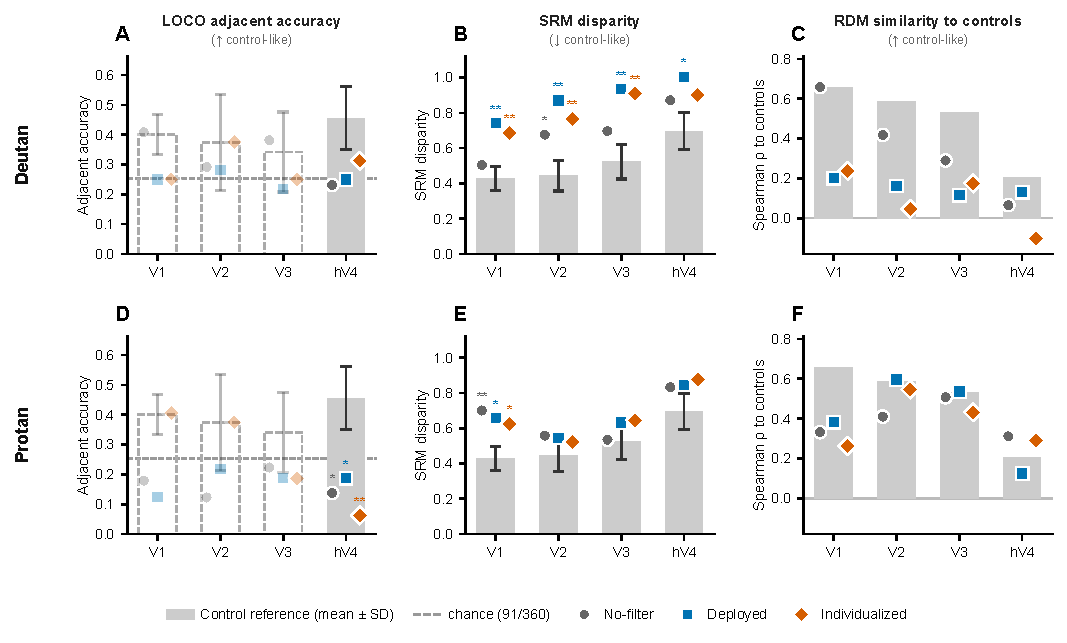
\includegraphics[width=\textwidth]{fig8_filter_eval}
  \caption{\textbf{Hue interpolation and representational geometry under each filter in the second
    session.} Rows: the deutan participant (A--C) and the protan participant (D--F). Markers: no-filter (gray circle, Session-1 baseline),
    deployed accessibility filter (blue square), individualized filter (orange diamond).
    Every panel is run-matched, with the control reference and the unfiltered baseline built from four
    runs to match the filter conditions (Supplementary~\cref{app:filter_eval}).
    \textbf{(A, D)} LOCO adjacent accuracy, the proportion of predictions within one hue step of
    the target ($\uparrow$ control-like). Gray bars give the control mean $\pm$ SD and the dashed
    line the analytic chance level of $0.25$. hV4 is the region credited with interpolation
    (Section~\ref{sec:results:loco}); V1--V3 are rendered muted with dashed outlines and are
    shown for comparison only, carrying no interpretation.
    \textbf{(B, E)} SRM disparity into the control-derived shared space ($\downarrow$ control-like). Gray bars give
    the control mean $\pm$ SD.
    \textbf{(C, F)} Shared-space RDM similarity to controls ($\uparrow$ control-like). The gray bar is the control
    leave-one-out self-consistency, a single value, so these panels carry no error bar or significance marker.
    Stars in (A, B, D, E) give one-tailed Crawford--Howell single-case deviations from the control
    distribution ($^{*}p<.05$, $^{**}p<.01$, $^{***}p<.001$); in (A, D) they appear at hV4 only.}
  \label{fig:filter_eval}
\end{figure}

\paragraph{Interpolation.}
At hV4 the individualized filter raised interpolation in the deutan participant and lowered it in the protan participant (Fig.~\ref{fig:filter_eval}A, D). In the deutan participant it was the only one of the three conditions to exceed the analytic chance level. In the protan participant it gave the lowest of the three conditions, and all three fell below chance. Per-condition values and single-case effect sizes are in Supplementary Table~\ref{tab:exp2_geometry}.

\paragraph{Geometry.}
Both filters left the representational geometry short of the control level, and the direction of the filter effect reversed between participants (Fig.~\ref{fig:filter_eval}B, C, E, F). In the deutan participant both filters moved the geometry away from the control reference on disparity and on RDM similarity. In the protan participant both filters reduced disparity, while RDM similarity rose under the deployed filter and fell under the individualized one. Neither index attributes the geometric change to individualization (Supplementary Table~\ref{tab:exp2_geometry}).


% Discussion Section
% Discussion Section v3 — last revised 2026-09-04
% Reframe: CVD color deficit = individual-specific GEOMETRIC DISTORTION of
%   cortical color representation. RDM = structure, LOCO = functional consequence.
%   Neural + psychophysical measurements JOINTLY ground an individualized correction.
%
% Spine: 3 contributions (paragraph map: discussion_structure_v3.md §2)
%   C1 structural/geometric distortion (RQ1)          — ¶2
%   C2 individualized filter from cortical geometry   — ¶3-¶8
%   C3 filter evaluation, second session (2 cases)    — ¶9-¶11
%
% 17 paragraphs. Renumber discussion_structure_v3.md §2 whenever this changes,
% or the next /revise-draft drift check is meaningless.
%
% Removed from v2: upstream-input-rejection paragraph; detection-correction
%   "divergence" falsifier + §S14 cosine statistic.
%
% Revision log
%   2026-06-08  v3 drafted (C3 was then a forward-looking Phase-3 TODO).
%   2026-08-05  BLUF/NEGA pass over P1-P10 (discussion_v3_revision_checklist.md).
%   2026-08-06  Phase-3 data folded in: C3 became a reported evaluation.
%               /revise-draft round 1 -> revision_report_2026-08-06.md.
%               §7 splits at former L29/L34/L43; control terminology unified.
%   2026-08-07  Round 2 fixes (¶1); "behavioral" -> "psychophysical" throughout.
%   2026-09-04  P2 compressed (205 -> 145); Limitations 5 paragraphs -> 2 (513 -> 234),
%               preprocessing-dependence detail left to Results/Supplementary; Conclusion -> one
%               paragraph in Kwon 2025 form (words_trimming.md §4).
%
% Brief / evidence pack / constraints: discussion_structure_v3.md

\section{Discussion}
\label{sec:discussion}

In both CVD participants categorical color identification was preserved while continuous hue interpolation fell to chance at hV4, and the hue geometry of both departed from the control reference by more than the controls departed from one another. We modeled that distortion as a hue rotation about the subtype confusion axis and the S-cone axis, fitted it to each participant's own neural and psychophysical measurements, and inverted it into a per-person stimulus-space filter evaluated in a second session. Under the individualized filter the elevated discrimination thresholds of both participants returned to the control range, the deployed accessibility filter left two pairs deviant in the protan participant, and the neural endpoints varied by participant and by measure. Together these results locate the CVD deficit in continuous hue geometry, which categorical decoding does not detect, and they show that an individual's own cortical color representation can be inverted into a correction filter for that individual.

\subsection{A geometric distortion of cortical color representation}
Both CVD participants identified all eight hues well above chance at every region while their hue interpolation fell to chance at hV4, the only region where the controls interpolated above their color-label null. The preserved identification and the reduced interpolation each held under head-motion correction (Section~\ref{sec:results:loco}; Supplementary~\cref{app:uncorrected}). Procrustes disparity from the control reference was elevated in both participants, while the region carrying the largest deviation was unstable across preprocessing in the deutan participant, leaving the cortical locus of the distortion undetermined (Section~\ref{sec:results:geometry}).

\subsection{A neurally grounded, individualizable correction filter}
The filter is the stimulus-space pre-image of the fitted distortion. For each intended color it substitutes the displayed hue that the participant's own cortical transformation maps onto that intended color (Methods~\S\ref{sec:methods:filter}). Each participant's loss combination was fixed beforehand by the pre-specified three-gate procedure over held-out control resamples (Methods~\S\ref{sec:methods:selection}). The two fitted corrections differed in magnitude and in direction, which parallels psychophysical evidence that hue perception varies markedly across anomalous trichromats \parencite{emery2021}. Their parameters come from each individual's own measurements rather than from a subtype average, and the neural and psychophysical terms are not redundant. The neural term located a confusion-axis rotation that the psychophysical loss alone left near zero, and it narrowed the parameter uncertainty in both participants (Section~\ref{sec:results:neural_role}). To our knowledge this is the first color-correction filter derived from an individual's cortical color representation rather than from a retinal model. Earlier inversions of cortical encoding models synthesized images that maximize the response of chosen units \parencite{bashivan2019} or voxels \parencite{shinkle2025} rather than the arrangement of colors within a region.

The fits recover the sign of the dominant confusion-axis term. No recovery check established the magnitude on either axis, and in the protan participant even that sign depends on the reduction basis and on the preprocessing pipeline (Supplementary~\cref{app:identifiability}, \cref{app:fit_stability}). With one participant per subtype, individual and subtype differences also remain confounded. Fixing those parameters therefore calls for a larger sample and a fitting procedure whose solution is stable across these analysis choices. This framework is built to support that analysis.

\subsection{Filter evaluation}
In the psychophysical evaluation both filters removed the deutan participant's baseline threshold deficit, whereas in the protan participant the individualized filter left every hue-discrimination pair within the control range and preserved color identification accuracy while the deployed filter left two pairs deviant and lowered identification. The psychophysical advantage of the individualized filter therefore appeared in the protan participant only. The neural evaluation differed across measures. Hue interpolation at hV4 rose under the individualized filter in the deutan participant and fell in the protan participant, while the early-visual geometry moved in the opposite direction within each participant and did so under both filters alike, so neither shift was specific to the individualized correction. Representational similarity to the controls was higher under the deployed filter in both participants, and the geometry of both remained displaced from the control reference under either filter (Section~\ref{sec:results:filter_eval}).

Early-visual geometry and hV4 interpolation lie at different levels of the visual hierarchy and can vary independently, so the disagreement alone does not show which readout tracks the correction. With one participant per subtype these neural endpoints remain inconclusive, and establishing whether either pattern generalizes requires replication in more individuals within each subtype on a refined neural endpoint.

\subsection{Limitations}
The CVD sample is $N = 2$, one participant per subtype, with subtype assigned from Ishihara plates rather than anomaloscopy. Single-case statistics \parencite{crawford1998} support inference about each individual, and the seven controls serve only to place each CVD estimate relative to the control range. Claims about deutan or protan subtypes, and the separation of a per-person correction from a subtype-average one, require several participants within each subtype. The fitted parameters are reported without confidence intervals, because six runs per participant are too few for stable resampling.

Several estimates depend on analysis choices, and the measurements cover a narrow stimulus range. The regional attribution of the geometric distortion and the sign of the protan confusion-axis term vary with preprocessing and with the reduction basis, so we report the geometry as descriptive and select filter targets by held-out test-loss (Section~\ref{sec:results:geometry}; Supplementary~\cref{app:uncorrected}, \cref{app:fit_stability}, \cref{app:geometry_validity}). The two neural loss terms read different regions and moved in different directions at evaluation, so no neural endpoint is yet stable enough for a larger study, and the assumption that shifting cortical geometry toward the control reference shifts perception with it remains untested. The stimuli occupied a single lightness and chroma locus, lightness was equated for the standard observer rather than for each participant, and the scanner task directed attention away from color \parencite{brouwer2013}. Extending the correction to natural scenes and to attended color requires refitting under those conditions.

\subsection{Conclusion}
This study shows that in two individuals with CVD categorical hue identification was preserved while continuous hue interpolation at hV4 was reduced, and that an individual's own cortical color representation can be inverted into a per-person stimulus-space correction filter. In the future, we anticipate that scaling this procedure to larger CVD and control samples will quantify the cortical color distortions of CVD, yield a fitting procedure which is stable across preprocessing and analysis choices, and deliver individualized filters whose effect on color perception can be established.



%%%%%%%%%%%%%%%%%%%%%%%%%
% Back matter — Imaging Neuroscience order and section names.
%
% IN Guide for Authors mandates, in this order:
%   Data and Code Availability (mandatory) → Author Contributions (mandatory)
%   → Funding (optional) → Declaration of Competing Interests (mandatory)
%   → Acknowledgements (optional) → Supplementary → References.
% The previous arrangement followed Elsevier/NeuroImage and has been replaced.
%
% STATUS: remaining \todo{} blocks render in red and MUST be resolved before
% submission. Checklist: SUBMISSION_CHECKLIST_IMAGING_NEURO.md
%%%%%%%%%%%%%%%%%%%%%%%%%

\clearpage

% Declaration of the use of AI.
% Required as a standalone end-matter section by the Imaging Neuroscience Guide
% for Authors, which asks for (i) the role AI played in planning and carrying out
% the research, (ii) the exact tools and version numbers, and (iii) the role AI
% played in generating figures. The guide also requires the same disclosure in
% the cover letter -- keep the two worded identically.
%
% Supersedes the paragraph that previously sat unlabelled after Acknowledgements
% and asserted "No figure, text, statistical result, or numerical value in this
% article was produced by an AI tool". That sentence was inaccurate: AI tools
% were used to reword author-written draft text and to check spelling and
% grammar. Scope confirmed by the authors 2026-09-01.
\section*{Declaration of the use of AI}

With respect to the research described in this paper, AI tools played no part in
the study design, in the choice of analyses, or in the interpretation of the
results. AI-based coding assistants were used to review the analysis code and to
check its correctness against the committed data. Every result reported here was
produced by executing that code, and the authors verified the outputs.

With respect to the preparation of the manuscript, the authors used AI tools to
check spelling and grammar and to reword draft text written by the authors. All
statistical results and numerical values reported in the paper were taken from
the analysis outputs rather than from an AI tool.

No figure contains AI-generated content. Every figure is produced by the analysis
and figure scripts released with the paper.

The AI tool used was Claude Code 2.1.259 (Anthropic), running the Claude Opus 5
model.

The authors take full responsibility for the content of this article, including
any part prepared with the assistance of these tools.

\section*{Data and Code Availability}

All analysis and preprocessing code needed to reproduce the reported results is
openly available at \url{https://github.com/Transconnectome/colorBlind_analysis}
\todo{[FILL AT SUBMISSION] and archived at Zenodo DOI xx.xxxx/zenodo.xxxxxxx.
IN asks for a persistent identifier; make the repository public and mint a
release DOI before submission so that reviewers can access it.}

% Deposit of derived data was examined against the approved protocol and the
% signed consent form (docs/archive/final_IRB.pdf, docs/archive/[변경2차] IRB
% No. 2510_002-023.pdf) on 2026-08-16 and is NOT permitted: the protocol places
% all study data in a principal-investigator-only encrypted store, and the
% consent form contains no secondary-use, third-party-provision, or public
% deposit clause. Open deposit would require a new ethics submission. The
% restricted-access statement below is therefore the whole of the data half.

The neuroimaging and behavioral data cannot be shared openly. The protocol
approved by the Seoul National University Institutional Review Board (SNUIRB
No.~2510/002-023), and the written consent obtained under it, place all study
data in an encrypted store to which the principal investigator controls access,
and neither document provides for secondary use by third parties or for deposit
in a public repository. Under Article 16(3) of the Seoul National University
Research Ethics Guidelines, the de-identified study data are retained for five
years and, thereafter, for as long as the principal investigator can maintain
custody of them, so that the integrity of the reported analyses can be verified.
Requests for access should be directed to the principal investigator (Jiook Cha,
connectome@snu.ac.kr) and are granted subject to (i) a formal data sharing
agreement between the requesting institution and Seoul National University,
(ii) approval of the intended use by the requesting researcher's local ethics
committee, and (iii) a short project outline describing that use; a request that
falls outside the scope of the original consent additionally requires a new
submission to the Seoul National University Institutional Review Board.
Co-authorship is not a condition of access. Requests are answered within eight
weeks.

\section*{Author Contributions}

% Format follows the published Imaging Neuroscience article used as this
% manuscript's style reference: Kwon et al., Imaging Neuroscience 3 (2025),
% doi:10.1162/imag_a_00440, whose statement names each author in full and states
% that author's roles in prose ("Junbeom Kwon: Junbeom Kwon served as the primary
% investigator and was instrumental in ...").
%
% This supersedes the earlier initials-plus-semicolons form modeled on
% doi:10.1162/IMAG.a.55. Both forms are published IN practice; the full-name form
% was chosen by the authors 2026-09-04. Every CRediT role carried by the previous
% version is preserved below, in CRediT vocabulary:
%   Jinil Kim          Conceptualization, Methodology, Software, Validation,
%                      Formal analysis, Investigation, Data curation,
%                      Visualization, Project administration, Funding
%                      acquisition, Writing---original draft,
%                      Writing---review & editing
%   Albert Minkue Cho  Conceptualization, Methodology, Formal analysis,
%                      Investigation, Data curation, Project administration,
%                      Funding acquisition, Writing---review & editing
%   Jungwoo Seo        Conceptualization (supporting), Investigation, Funding
%                      acquisition, Writing---review & editing
%   Jiook Cha          Conceptualization, Methodology, Validation, Resources,
%                      Supervision, Funding acquisition, Writing---review &
%                      editing
% The Editorial Manager submission form collects the same roles as taxonomy
% terms with degree-of-contribution qualifiers; keep the two consistent.
%
% Roles supplied by the corresponding author 2026-08-17. Two mappings were
% applied, because CRediT has no matching term for the labels given:
%   "result interpretation" -> Formal analysis (CRediT: "application of
%       statistical, mathematical, computational, or other formal techniques to
%       analyze or synthesize study data"); interpretation has no separate role.
%   "data collection" / "recruitment" -> Investigation.
% Funding acquisition is assigned to all four authors: the award is a university
% undergraduate programme applied for jointly, which the closing sentence states.

Jinil Kim: Jinil Kim served as the primary investigator and led the
conceptualization and the methodology of the study. Jinil Kim wrote the analysis
software, collected the neuroimaging and psychophysical data, and curated and
validated them. Jinil Kim also led the formal analysis and the interpretation of
the results, produced the figures, administered the project, and drafted the
original manuscript.

Albert Minkue Cho: Albert Minkue Cho contributed to the conceptualization and the
methodology of the study and took part in participant recruitment and data
collection and curation. Albert Minkue Cho also carried out part of the formal
analysis, shared responsibility for project administration, and reviewed and
edited the manuscript.

Jungwoo Seo: Jungwoo Seo contributed to the conceptualization of the study in a
supporting role and took part in data collection. Jungwoo Seo also reviewed and
edited the manuscript.

Jiook Cha: Jiook Cha, as the corresponding author, took on a supervisory role,
providing overall guidance and direction for the project. Jiook Cha contributed
to the conceptualization and the methodology, validated the analyses, and
provided the imaging and computational resources on which the study depended.
Jiook Cha also reviewed and edited the manuscript.

All four authors applied jointly for the funding that supported this work.

% Both sampled Imaging Neuroscience research articles carry a short back-matter
% "Ethics" section in addition to the statement in Methods (doi:10.1162/IMAG.a.55,
% doi:10.1162/imag_a_00455). The Guide for Authors does not list it, but house
% practice does, so it is included here; the fuller statement stays in Methods.
\section*{Ethics}

The Seoul National University Institutional Review Board approved the study
(SNUIRB No.~2510/002-023), which was conducted in accordance with the
Declaration of Helsinki. Written informed consent was obtained from all
participants for being included in the study.

\section*{Funding}

% Funding text confirmed by the authors 2026-09-01. It supersedes the earlier
% statement naming the Independent Research Support Program of the College of
% Liberal Studies, which was taken from the approved protocol
% (docs/archive/final_IRB.pdf p.2) and is no longer the funding of record.
% The only editorial change to the supplied wording is punctuation: the supplied
% text read "... (2025). and Undergraduate Social Science Research Grant ...",
% which is joined here into a single sentence.
This work was supported by the SNU Student-directed Education Undergraduate
Research Program through the SNU College, Seoul National University (2025), and
by the Undergraduate Social Science Research Grant through the College of Social
Sciences, Seoul National University (2026).

\section*{Declaration of Competing Interests}

The authors declare that they have no known competing financial interests or
personal relationships that could have appeared to influence the work reported
in this paper. No patent has been filed on the correction filter described here,
and no author has a financial relationship with a supplier of color-correction
eyewear or display software.

\section*{Acknowledgements}

Imaging was carried out at the Seoul National University Brain Imaging Center,
and the authors thank its staff for their support. The authors also thank
Juhyoung Ryu for assistance with coregistration during preprocessing, Eunhwi Lee
for support with the experimental design, and Seung Yun Choi for revising the
experiment documents.

%%%%%%%%%%%%%%%%%%%%%%%%%
% References
%%%%%%%%%%%%%%%%%%%%%%%%%

\printbibliography



%%%%%%%%%%%%%%%%%%%%%%%%%
% Supplementary Methods
%%%%%%%%%%%%%%%%%%%%%%%%%

\clearpage
\section*{Supplementary Methods}
% ============================================================================
% Supplementary Material — consolidated 2026-08-07
% Single file replacing the previous split across Methods/supplementary_content.tex
% and four files in Supplementary/. Section text was moved verbatim; only the
% per-file header comments below were relocated to mark provenance.
% Included from main.tex as: % ============================================================================
% Supplementary Material — consolidated 2026-08-07
% Single file replacing the previous split across Methods/supplementary_content.tex
% and four files in Supplementary/. Section text was moved verbatim; only the
% per-file header comments below were relocated to mark provenance.
% Included from main.tex as: % ============================================================================
% Supplementary Material — consolidated 2026-08-07
% Single file replacing the previous split across Methods/supplementary_content.tex
% and four files in Supplementary/. Section text was moved verbatim; only the
% per-file header comments below were relocated to mark provenance.
% Included from main.tex as: \input{Supplementary/supplementary}
% Superseded sources: docs/PAPER/Supplementary/archive/ (gitignored)
% ============================================================================

\renewcommand{\thetable}{S\arabic{table}}\setcounter{table}{0}


% ========== Section 1: Session-1 hue-discrimination thresholds ==========

\suppsection{Session-1 hue-discrimination thresholds}{app:jnd_baseline}

Session-1 threshold elevations followed each participant's subtype (\cref{tab:jnd_baseline}). The threshold is the staircase level $t$, the fraction of the pair's full CIE $LCh$ separation at which the two discs were discriminated (\S\ref{sec:methods:psychophysical}), so smaller values indicate finer discrimination. The ratio $\gamma$ divides the participant's threshold by the control mean, and $z$ expresses the same difference in control standard deviations over the seven controls. Pairs are grouped by the axis each was chosen to probe, and that assignment was fixed before any threshold was collected.

Each pair was measured by two interleaved staircases from starting levels $t = 0.8$ and $t = 0.5$, both following a 1-up/1-down rule with a step of $0.15$ until the second reversal and $0.03$ thereafter. A staircase terminated at eight reversals and at least 20 trials, extended by two further reversals whenever the SD of the last six reversal levels exceeded $0.10$.

Elevation localized to the axis each participant's subtype predicts. The deutan participant exceeded $z = +4$ on both deutan-axis pairs and on the yellow--purple S-cone pair, and the protan participant exceeded the control range on the protan-axis pair green--blue alone. Both participants remained inside the control range on the $180^\circ$ control pair, which places the elevation on specific axes rather than on overall sensitivity. These thresholds enter the psychophysical loss atoms of \S\ref{sec:methods:candidates}, and the same eight pairs supply the pre-filter baseline of the filter evaluation (\S\ref{sec:results:filter_eval}).

\begin{table}[h]
\centering
\caption{Session-1 hue-discrimination thresholds without a filter. The control column is the mean $\pm$ SD over the seven controls. $\gamma$ is the ratio to the control mean and $z$ the deviation in control standard deviations. Bold: $|z| \geq 2$. Two staircases returned an incorrect response at the largest presentable separation, both of them the deutan participant's orange--yellow pair, so that threshold is a lower bound rather than an estimate. It is the only such pair among the 208 staircases collected in this study.}
\label{tab:jnd_baseline}
\setlength{\tabcolsep}{4pt}
\begin{tabular}{llcccccccc}
\toprule
& & \multicolumn{2}{c}{Controls ($n = 7$)} & \multicolumn{3}{c}{Deutan} & \multicolumn{3}{c}{Protan} \\
\cmidrule(lr){3-4}\cmidrule(lr){5-7}\cmidrule(lr){8-10}
Axis probed & Pair & mean & SD & $t$ & $\gamma$ & $z$ & $t$ & $\gamma$ & $z$ \\
\midrule
Deutan confusion & orange--yellow & $0.278$ & $0.135$ & $0.840$ & $\mathbf{3.02}$ & $\mathbf{+4.15}$ & $0.193$ & $0.69$ & $-0.63$ \\
                 & yellow--green  & $0.090$ & $0.044$ & $0.278$ & $\mathbf{3.10}$ & $\mathbf{+4.32}$ & $0.128$ & $1.42$ & $+0.87$ \\
\midrule
Protan confusion & green--blue    & $0.079$ & $0.032$ & $0.078$ & $0.98$ & $-0.06$ & $0.155$ & $\mathbf{1.95}$ & $\mathbf{+2.36}$ \\
                 & cyan--magenta  & $0.042$ & $0.017$ & $0.040$ & $0.95$ & $-0.13$ & $0.038$ & $0.89$ & $-0.28$ \\
\midrule
S-cone           & yellow--purple & $0.022$ & $0.006$ & $0.063$ & $\mathbf{2.87}$ & $\mathbf{+6.70}$ & $0.028$ & $1.26$ & $+0.94$ \\
                 & blue--purple   & $0.164$ & $0.093$ & $0.120$ & $0.73$ & $-0.48$ & $0.148$ & $0.90$ & $-0.18$ \\
                 & red--orange    & $0.124$ & $0.072$ & $0.063$ & $0.50$ & $-0.85$ & $0.075$ & $0.61$ & $-0.68$ \\
\midrule
Control          & red--cyan      & $0.034$ & $0.015$ & $0.015$ & $0.45$ & $-1.23$ & $0.015$ & $0.45$ & $-1.23$ \\
\midrule
\multicolumn{7}{l}{Mean $|z|$ over the eight pairs \quad Deutan $2.24$ \quad Protan $0.90$} & & & \\
\bottomrule
\end{tabular}
\end{table}


The deutan orange--yellow threshold is a lower bound. Both of its staircases remained at the top of the presented range throughout and returned incorrect responses at the largest separation the task presents. Censoring understates the baseline deficit and therefore the improvement recorded under either filter, so the value is reported unadjusted.

\begin{table}[h]\centering\small
\caption{Both staircase estimates for every hue pair, given as high-start/low-start in units of the rendered separation. Bold marks the cells whose two estimates differ by more than 0.10. Thresholds reported elsewhere are the mean of the two.}
\label{tab:staircase_pairs}
\begin{tabular}{lcccccc}
\toprule
 & \multicolumn{3}{c}{Deutan} & \multicolumn{3}{c}{Protan} \\
\cmidrule(lr){2-4}\cmidrule(lr){5-7}
Pair & Session 1 & Deployed & Individualized & Session 1 & Deployed & Individualized \\
\midrule
red--orange & 0.060/0.065 & 0.160/0.210 & 0.140/0.130 & 0.075/0.075 & 0.110/0.145 & 0.070/0.055 \\
orange--yellow & 0.870/0.810 & 0.080/0.110 & 0.060/0.032 & 0.175/0.210 & 0.170/0.185 & \textbf{0.715/0.200} \\
yellow--green & 0.280/0.275 & 0.090/0.075 & 0.145/0.165 & 0.125/0.130 & 0.057/0.050 & 0.055/0.065 \\
green--blue & 0.065/0.090 & 0.150/0.110 & 0.045/0.060 & 0.145/0.165 & 0.260/0.225 & 0.135/0.080 \\
blue--purple & 0.115/0.125 & 0.050/0.095 & 0.110/0.200 & 0.125/0.170 & 0.135/0.110 & 0.150/0.105 \\
yellow--purple & 0.060/0.065 & 0.015/0.020 & 0.035/0.025 & 0.020/0.035 & 0.020/0.015 & 0.015/0.015 \\
red--cyan & 0.015/0.015 & 0.040/0.018 & 0.015/0.045 & 0.015/0.015 & 0.030/0.040 & 0.020/0.025 \\
cyan--magenta & 0.035/0.045 & 0.030/0.025 & 0.040/0.033 & 0.040/0.035 & 0.150/0.140 & 0.015/0.020 \\
\bottomrule\end{tabular}\end{table}

The two staircases of a pair agreed closely (\cref{tab:staircase_pairs}). They differed by a median of $0.015$ across the $104$ pairs, and three cells exceeded $0.10$. The largest, at $0.515$, is the protan participant's orange--yellow pair under the individualized filter, where one track settled at $0.715$ after answering correctly at a four-fold smaller separation earlier in the same block while its partner converged at $0.200$ on the same rendered stimuli. We attribute that cell to a single lapse and report every threshold as the unadjusted mean of the two tracks. Restricting it to the converged track would move the cell from $z = +1.33$ to $z = -0.58$ and the participant's mean $|z|$ from $0.93$ to $0.84$.



% --------------------------------------------------------------------------
% ==== Sections carrying a "% ========== Section N ==========" banner below
%      (was Methods/supplementary_content.tex, archived) ====
% --------------------------------------------------------------------------
% Supplementary Methods - Content Only
% To be included via \input{Methods/supplementary_content}


% --------------------------------------------------------------------------
% ==== S2  (was Supplementary/S17_uncorrected_artifacts.tex) ====
% --------------------------------------------------------------------------
% Supplementary S1 — Preprocessing pipelines and sensitivity analyses
% 2026-08-07
% Scope: slice timing, head motion, susceptibility distortion were all left
%   uncorrected in the analyzed pipeline. Motion has a sensitivity analysis;
%   distortion and coregistration are argued on structural grounds.
% Source numbers: analysis/phase2_SRM_across_between/results/RESULTS_MOTION_ARMS_2026-08-05.md
%   Coregistration stability: docs/PAPER/METHODS_REVISION_STATUS_2026-08-07.md §3

\suppsection{Preprocessing pipelines and sensitivity analyses}{app:uncorrected}

\paragraph{The two pipelines.}
Every neural endpoint of the first session was computed under two pipelines. The primary pipeline resampled each functional volume once by a transform identical for every volume in a run. The second composed each volume's MCFLIRT rigid-body realignment matrix with that transform before the same single resampling, so the two differ in the alignment method and share the number of resamplings. Head-motion correction lowered ROI temporal signal-to-noise ratio by $1.7$ to $2.7\%$. In both, the per-run linear and constant drift terms of the general linear model constituted the entire nuisance model, and both pipelines left slice timing, susceptibility distortion, and temporal filtering out. Within-run motion was estimated by registering every volume to its run's middle volume and summarized as framewise displacement \parencite{power2012}, with rotations converted to displacement on a 50\,mm sphere. Across the nine analyzed participants mean framewise displacement reached $0.318 \pm 0.044$\,mm (controls $0.313 \pm 0.042$, CVD $0.338 \pm 0.046$), and $16.2\%$ of volumes exceeded $0.5$\,mm.

\paragraph{Disparity under the two pipelines.}
The regional attribution of disparity depends on the pipeline (\cref{tab:motion_arms}). Procrustes disparity was recomputed under head-motion correction with every other element held fixed. The protan V1 elevation remained the largest deviation in that participant under both pipelines and weakened from $p = .007$ to $p = .077$. In the deutan participant the largest deviation moved from V2 to V1 and the V2 value reversed in sign. Under the leave-one-subject-out estimator the protan V1 cell of the primary pipeline reached significance alone.

\begin{table}[h]
\centering
\caption{Procrustes disparity by participant and region under head-motion correction. Entries give the Crawford--Howell one-tailed $t$ with $p$ in parentheses, against the control leave-one-out distribution ($n = 7$), for the common-space estimator and for the leave-one-subject-out estimator on which the inference rests. The primary pipeline appears in \cref{tab:disparity_loso}, which adds the case-control effect sizes. Individual cells of this grid are descriptive and support no claim in the main text.}
\label{tab:motion_arms}
\small
\begin{tabular}{llcc}
\toprule
Participant & Region & Crawford--Howell & Leave-one-subject-out \\
\midrule
Deutan & V1  & $2.4$ ($.027$) & $1.6$ ($.080$) \\
Deutan & V2  & $-1.0$ ($.825$) & $-0.6$ ($.723$) \\
Deutan & V3  & $0.6$ ($.293$) & $0.4$ ($.338$) \\
Deutan & hV4 & $0.4$ ($.351$) & $0.4$ ($.356$) \\
Protan & V1  & $1.6$ ($.077$) & $1.3$ ($.121$) \\
Protan & V2  & $1.0$ ($.186$) & $0.1$ ($.480$) \\
Protan & V3  & $1.1$ ($.151$) & $1.0$ ($.178$) \\
Protan & hV4 & $1.4$ ($.101$) & $1.1$ ($.159$) \\
\bottomrule
\end{tabular}
\end{table}

\paragraph{Classification and interpolation under the two pipelines.}
The two readouts dissociate under both pipelines (\cref{tab:interp_arms}). The control-group interpolation gate, the two single-case comparisons at hV4 (\S\ref{sec:results:loco}), and the eight-way classification readout (\S\ref{sec:results:loro}) were recomputed the same way. hV4 alone passes the control gate in both pipelines, and both participants remain below the control mean in both. Classification survives in both. The lowest CVD cell across the four regions reaches $0.375$ under the primary pipeline and $0.229$ under head-motion correction, $1.8$ times the $0.125$ chance level. Every single-case classification contrast stayed above $p = .10$ in both pipelines, and the single-case interpolation contrasts reached significance under the primary pipeline alone.

\begin{table}[h]
\centering
\caption{Hue-interpolation adjacent accuracy and eight-way classification accuracy under the two pipelines. Upper rows give the control interpolation mean with its $p$ against $1{,}000$ per-subject color-label permutations ($n = 7$; the permutation null mean is $0.35$ in both pipelines). Middle rows give each CVD participant's interpolation accuracy at hV4 with the one-tailed Crawford--Howell $p$ against the control distribution. Lower rows give classification accuracy at hV4, for which chance is $0.125$ and the Crawford--Howell test is two-tailed because the hypothesis is preservation; the control mean is listed for reference and is not tested. The primary-pipeline accuracies appear with their full four-region grid in \cref{tab:alignment}. Individual cells of this grid are descriptive and support no claim in the main text.}
\label{tab:interp_arms}
\begin{tabular}{lcccc}
\toprule
 & \multicolumn{2}{c}{Primary} & \multicolumn{2}{c}{Head-motion correction} \\
\cmidrule(lr){2-3}\cmidrule(lr){4-5}
 & Accuracy & $p$ & Accuracy & $p$ \\
\midrule
\multicolumn{5}{l}{\emph{Interpolation (LOCO adjacent accuracy)}} \\
Controls V1  & $0.393$ & $.164$ & $0.283$ & $.922$ \\
Controls V2  & $0.357$ & $.424$ & $0.381$ & $.228$ \\
Controls V3  & $0.339$ & $.586$ & $0.315$ & $.810$ \\
Controls hV4 & $0.456$ & $.011$ & $0.451$ & $.023$ \\
Deutan hV4 & $0.250$ & $.054$ & $0.354$ & $.242$ \\
Protan hV4 & $0.125$ & $.012$ & $0.271$ & $.108$ \\
\midrule
\multicolumn{5}{l}{\emph{Classification (LORO eight-way accuracy)}} \\
Controls hV4 & $0.488$ & --- & $0.569$ & --- \\
Deutan hV4 & $0.375$ & $.351$ & $0.583$ & $.905$ \\
Protan hV4 & $0.375$ & $.351$ & $0.396$ & $.197$ \\
\bottomrule
\end{tabular}
\end{table}

\paragraph{Session-2 endpoints under the harmonized arm.}
The second-session cortical readouts depend on the preprocessing arm, so we report both arms and treat every directional contrast in them as provisional. The session was reprocessed with the anatomical images harmonized to the first and with head-motion correction, and the fourteen pre-specified endpoints were recomputed within each arm, so the control reference and the Session-1 unfiltered anchor always come from the same reconstruction. The control reference moved from $0.456$ to $0.445$ in hV4 adjacent accuracy, whereas the single-participant, single-condition cells moved far more. Eight of the ten directional contrasts defined on the native voxel mask reversed between arms, as did five of the ten defined on the run-matched mask. The geometry indices moved less, and the four contrasts at the pre-specified target regions held in both arms. The psychophysical endpoints are independent of preprocessing and are unchanged.

\paragraph{Susceptibility distortion.}
Susceptibility distortion within the analyzed ROIs is predominantly subvoxel and spatially smooth, which places it outside the set of explanations for the observed differences in representational geometry across hue conditions. A gradient-echo field map was acquired in each session and linked to the functional runs through the BIDS \texttt{IntendedFor} field, and both pipelines left it unconsumed, so the data retain distortion along the right--left phase-encoding direction. Field-map-derived mean displacement within each analyzed ROI ranged from $0.01$ to $0.76$ voxels ($0.02$--$1.52$\,mm) across the nine participants. Within-ROI spatial variation is the component that distorts a pattern rather than translating it, and it reached $0.05$--$0.21$ voxels in eight participants and $0.38$ voxels ($0.76$\,mm) in the ninth. The residual cost is spatial, reducing the precision with which atlas-defined regions are assigned to functional voxels.

\paragraph{Registration.}
The functional series cover occipital cortex alone, so registration used mutual information initialized from the scanner-defined obliquity in the NIfTI header, which tolerates limited coverage and requires no white-matter boundary. Two standard routes were evaluated first and both were rejected. A container-based route through fMRIPrep failed at the coregistration stage on every attempt with these partial-coverage series. Boundary-based registration within the custom pipeline snapped the functional slab onto an incorrect tissue boundary on visual inspection, an error on the order of $10$\,mm, where the mutual-information solution stayed within about $1$\,mm of the visually verified position. Whole-brain overlap indices favor boundary-based registration on these data, but Dice and ROI-coverage measures respond to the extent of overlap rather than to the position of a partial slab within the brain, so the choice rests on the visual criterion.

The mutual-information optimum is shallow under this field of view. Across the runs of a single session, where the fitted transform should be identical, the mean pairwise displacement of the solution ranged from $0.9$ to $4.2$\,mm. Removing facial voxels from the anatomical image, which leaves the brain unchanged, moved the solution by $1.9$\,mm in the deutan participant and $9.4$\,mm in the protan participant. The transform is fixed within a run, so it enters the eight hues of a run as run-to-run noise alone, which is attenuated by averaging over the six runs. Rigid-body estimation and distortion correction are constrained just as weakly when little of the head is imaged, so acquisitions of this type would benefit from correction validated for partial coverage.


% ========== Section 3: Quality Control ==========

\suppsection{ROI coverage}{app:roi_coverage}

ROI coverage averaged $83.5\%$ (SD $22.7\%$) across the nine analyzed participants, and $99.5\%$ of ROI voxels showed reliable stimulus-evoked responses. Coverage was computed as the intersection of the Wang atlas ROIs (V1, V2, V3, hV4) with each participant's BOLD brain mask in MNI space, taken per participant as the mean over the four regions and six runs. Its lowest value in the sample was $30.8\%$. Every analyzed participant entered the downstream analyses.


% ========== Section 4: K-Selection ==========

\suppsection{Dimensionality selection for the shared response model}{app:dimensionality}

SRM used $k = 4$ at V1 and V2 and $k = 3$ at V3 and hV4, with cross-subject RDM Spearman correlations of $0.60$, $0.57$, $0.55$ and $0.32$. The reduced dimension was determined by leave-one-subject-out cross-validation over the candidate values 2 to 6 \parencite{cunningham2014}. On each of the seven folds, one control participant was withheld from SRM training and three quality metrics were computed for every candidate. RDM split-half reliability was the Spearman correlation between representational dissimilarity matrices built from the odd runs 1, 3, and 5 and the even runs 2, 4, and 6 of the withheld participant in SRM space. The remaining two metrics were the cross-subject RDM correlation and the reconstruction error. Candidates were ranked within each fold and metric, and the candidate with the best mean rank was selected.


% --------------------------------------------------------------------------
% ==== S5  Alternative decoders ====
% --------------------------------------------------------------------------
% Supplementary S4 — Decoder comparison
% 2026-08-07. Resolves the dangling "Appendix A" reference at methods_v2.tex:149.
% Source (all committed JSON, dataset token C010):
%   LORO  analysis/phase3_decoder_comparing/results/loro/srm/sub-{01..09}_performance_raw.json
%         results.{ROI}.{model}[fold].acc_exact, averaged over the six folds
%   LOCO  analysis/phase3_decoder_comparing/results/loco/srm/sub-{01..09}_loco.json
%         results.{ROI}.{model}.overall_adjacent_acc
%   config models: LDA, Ridge, KernelRidge, SVM, MLP, ForwardEncoding; rois V1 V2 V3 V4;
%   K recovered from amplitudes_srm.npy shapes (V1 4, V2 4, V3 3, hV4 3) since dim_k is null.
% Provenance of the correlation readout: present in the repo at b3ce74d (2026-01-27),
%   plan document 1634142 (2026-02-17); the LOCO run is 2026-02-22 and LORO 2026-02-26.
%   It was therefore inherited and then verified, NOT selected by this comparison.
% Deliberately excluded: FE_PopVec / FE_RidgeEnc / FE_GaussML / FE_RidgeReg vary the
%   readout rather than the decoder and have no committed numeric output; the ensemble
%   variants were retired at 3ec8e51 / a825a7d (2026-02-26); HybridMLP / HybridSVR ran
%   for LOCO only and so cannot be placed beside the LORO table.

\suppsection{Comparison with alternative decoders}{app:decoders}

The hue-channel basis model was adopted for its interpolation behavior rather than for its classification accuracy. We compared six decoders on the same SRM-aligned amplitudes under both cross-validation schemes, which separate them in opposite directions. The present analyses rest on the interpolation result.

Linear discriminant analysis classified held-out runs most accurately at every ROI (\cref{tab:loro_decoders}). Its control mean reached $0.878$ at V1 against a chance level of $0.125$, with the support vector machine next at $0.777$ and the hue-channel basis model at $0.542$. The ordering held at V2, V3 and hV4. Four of the six decoders exceeded chance at every ROI, so eight-way classification is recoverable by several readouts and favors none of them.

Interpolation to a held-out hue reverses the ordering at hV4, the ROI on which the main analyses rest (\cref{tab:loco_decoders}). The hue-channel basis model reached an adjacent accuracy of $0.470$ there, against a chance level of $0.25$ for its continuous-hue output. It is the only decoder whose control mean exceeds its own chance level, doing so at V1 ($0.360$), V2 ($0.283$) and hV4, with the widest margin at hV4. The classifiers remained below their $0.375$ chance level at every ROI, and ridge and kernel ridge remained below $0.25$ everywhere. The analytic chance level compares a decoder against a uniform prediction, whereas the stricter main-text criterion uses a color-label permutation null that preserves the covariance among voxels, and hV4 is the region that meets it (\S\ref{sec:results:loco}). The pattern follows from the model form. The hue-channel basis model represents a hue as activation over six tuned channels and can therefore evaluate a hue it never saw during training, whereas a classifier trained on seven discrete labels has no output unit for the eighth.

Two decoders produced constant outputs. Kernel ridge regression returned an adjacent accuracy of exactly $0.000$ in every participant, ROI and alignment, and the multilayer perceptron returned exactly the chance value with zero variance across participants, which is the signature of a constant prediction. We treat both as uninformative rather than competitive.

\begin{table}[h]
\centering
\caption{Eight-way classification accuracy under leave-one-run-out cross-validation, SRM-aligned amplitudes, chance $= 0.125$. control mean $\pm$ SD ($n = 7$), with the two CVD participants listed separately. Bold: highest control mean in the ROI. Three further variants sit outside this comparison: the ensemble decoders were retired from the pipeline, the two hybrid decoders were run for interpolation alone, and four alternative readouts of the hue-channel basis model vary the readout rather than the decoder.}
\label{tab:loro_decoders}
\begin{tabular}{llccc}
\toprule
ROI & Decoder & Controls (mean $\pm$ SD) & Deutan & Protan \\
\midrule
V1 & LDA & $\mathbf{0.878 \pm 0.050}$ & 1.000 & 0.854 \\
   & SVM & $0.777 \pm 0.062$ & 0.979 & 0.771 \\
   & Hue-channel basis & $0.542 \pm 0.106$ & 0.604 & 0.625 \\
   & Ridge & $0.399 \pm 0.054$ & 0.354 & 0.250 \\
   & Kernel ridge & $0.393 \pm 0.064$ & 0.271 & 0.292 \\
   & MLP & $0.128 \pm 0.008$ & 0.125 & 0.125 \\
\midrule
V2 & LDA & $\mathbf{0.830 \pm 0.047}$ & 0.917 & 0.854 \\
   & SVM & $0.759 \pm 0.136$ & 0.875 & 0.833 \\
   & Hue-channel basis & $0.545 \pm 0.077$ & 0.458 & 0.438 \\
   & Ridge & $0.372 \pm 0.097$ & 0.458 & 0.250 \\
   & Kernel ridge & $0.330 \pm 0.066$ & 0.313 & 0.250 \\
   & MLP & $0.149 \pm 0.031$ & 0.125 & 0.125 \\
\midrule
V3 & LDA & $\mathbf{0.726 \pm 0.064}$ & 0.750 & 0.771 \\
   & SVM & $0.631 \pm 0.144$ & 0.813 & 0.667 \\
   & Hue-channel basis & $0.449 \pm 0.065$ & 0.375 & 0.313 \\
   & Ridge & $0.173 \pm 0.068$ & 0.292 & 0.229 \\
   & Kernel ridge & $0.158 \pm 0.052$ & 0.208 & 0.333 \\
   & MLP & $0.122 \pm 0.008$ & 0.125 & 0.125 \\
\midrule
hV4 & LDA & $\mathbf{0.658 \pm 0.092}$ & 0.813 & 0.729 \\
   & SVM & $0.598 \pm 0.085$ & 0.813 & 0.667 \\
   & Hue-channel basis & $0.423 \pm 0.072$ & 0.354 & 0.354 \\
   & Ridge & $0.319 \pm 0.114$ & 0.146 & 0.250 \\
   & Kernel ridge & $0.277 \pm 0.093$ & 0.042 & 0.188 \\
   & MLP & $0.125 \pm 0.000$ & 0.125 & 0.125 \\
\bottomrule
\end{tabular}
\end{table}

\begin{table}[h]
\centering
\caption{Adjacent accuracy under leave-one-color-out cross-validation, SRM-aligned amplitudes. control mean $\pm$ SD ($n = 7$), with the two CVD participants listed separately. Chance depends on the output space of the decoder. The hue-channel basis, ridge and kernel ridge return a continuous hue, so a uniform prediction lands within the $45^\circ$ tolerance on 91 of 360 draws and chance is $0.25$. The LDA, SVM and MLP classifiers return one of the eight stimulus hues, for which the tolerance admits 3 of 8 and chance is $0.375$. The constant-output MLP sits at exactly $0.375$ at V1 and V2, which confirms the classifier value. Bold: the largest margin above the applicable chance level. Kernel ridge and the MLP are constant-output rows, noted in the text. The hue-channel-basis rows of this table and of \cref{tab:loro_decoders} constitute the SRM-space readouts referred to in \cref{app:alignment}.}
\label{tab:loco_decoders}
\begin{tabular}{llccc}
\toprule
ROI & Decoder & Controls (mean $\pm$ SD) & Deutan & Protan \\
\midrule
V1 & Hue-channel basis & $0.360 \pm 0.098$ & 0.313 & 0.250 \\
   & LDA & $0.268 \pm 0.074$ & 0.375 & 0.167 \\
   & SVM & $0.226 \pm 0.078$ & 0.375 & 0.229 \\
   & Ridge & $0.039 \pm 0.053$ & 0.146 & 0.000 \\
   & MLP & $0.375 \pm 0.012$ & 0.375 & 0.375 \\
   & Kernel ridge & $0.000 \pm 0.000$ & 0.000 & 0.000 \\
\midrule
V2 & Hue-channel basis & $0.283 \pm 0.101$ & 0.333 & 0.063 \\
   & LDA & $0.327 \pm 0.088$ & 0.313 & 0.417 \\
   & SVM & $0.318 \pm 0.108$ & 0.250 & 0.396 \\
   & Ridge & $0.054 \pm 0.083$ & 0.021 & 0.000 \\
   & MLP & $0.375 \pm 0.000$ & 0.396 & 0.375 \\
   & Kernel ridge & $0.000 \pm 0.000$ & 0.000 & 0.000 \\
\midrule
V3 & Hue-channel basis & $0.220 \pm 0.100$ & 0.354 & 0.125 \\
   & LDA & $0.220 \pm 0.081$ & 0.271 & 0.333 \\
   & SVM & $0.208 \pm 0.103$ & 0.250 & 0.229 \\
   & Ridge & $0.000 \pm 0.000$ & 0.000 & 0.000 \\
   & MLP & $0.250 \pm 0.000$ & 0.250 & 0.250 \\
   & Kernel ridge & $0.000 \pm 0.000$ & 0.000 & 0.000 \\
\midrule
hV4 & Hue-channel basis & $\mathbf{0.470 \pm 0.130}$ & 0.271 & 0.104 \\
   & LDA & $0.280 \pm 0.144$ & 0.146 & 0.229 \\
   & SVM & $0.253 \pm 0.126$ & 0.167 & 0.208 \\
   & Ridge & $0.000 \pm 0.000$ & 0.000 & 0.000 \\
   & MLP & $0.250 \pm 0.000$ & 0.250 & 0.250 \\
   & Kernel ridge & $0.000 \pm 0.000$ & 0.000 & 0.000 \\
\bottomrule
\end{tabular}
\end{table}
The encoding model transfers to a held-out control better than to a CVD participant. A control-trained model applied to a held-out control reached a mean accuracy of $0.526$ over 28 subject-by-ROI cells, and the same model applied to a CVD participant reached $0.432$ over 8 cells (Mann--Whitney $U = 163.5$, $p = 0.052$, rank-biserial $r = 0.46$). Both destinations exceed the $0.125$ chance level, and the lowest single cell reached $0.271$. This comparison spans participants and is therefore computed in the SRM-aligned space, unlike the within-subject readouts of \cref{app:alignment}.


% ========== Section 6: GCV Details ==========

\suppsection{Generalized cross-validation for the ridge penalty}{app:gcv}

The ridge penalty applies to the encoding direction alone. Hue decoding uses the unregularized pseudoinverse, because a ridge penalty on the channel-to-voxel weights degrades the decoding readout (\cref{app:decoders}). The regularization parameter $\alpha$ was selected by generalized cross-validation \parencite{golub1979}, which approximates leave-one-out cross-validation at a fraction of its cost. We implemented it directly from the singular value decomposition of the channel design matrix, searching the grid $\{10^{-3}, 10^{-2}, 10^{-1}, 1, 10, 10^{2}, 10^{3}\}$. A single $\alpha$ was selected per fit by minimizing the GCV score,

\begin{equation}
\text{GCV}(\alpha) = \frac{\overline{\|Y - \hat{Y}\|_2^2}}{\left(1 - \text{tr}(H)/n\right)^2}
\end{equation}

where $C$ denotes the channel design matrix, $Y$ the observed responses of all voxels in the region, $\hat{Y}$ the ridge prediction, $H = C(C^T C + \alpha I)^{-1}C^T$ the hat matrix, and $n$ the number of training samples.
The squared residuals are averaged over both samples and voxels, so the selected penalty is shared across the voxels of a region.


% ========== Section 7: Cross-validation and metrics ==========

\suppsection{Cross-validation procedures and evaluation metrics}{app:cv_metrics}

\paragraph{Cross-run alignment and leakage control.}
The fixed-reference alignment bounds the leakage that a nested alignment could introduce. The run-level Procrustes alignment (\S\ref{sec:methods:roi}) maps runs 2--6 onto a fixed run-1 reference by an orthogonal rotation that uses no stimulus labels, so the alignment frame is defined independently of the held-out run or hue. Re-estimating the alignment inside each fold raised hue-channel-basis LORO accuracy from $0.545$ to $0.578$. Leakage in the fixed-reference pipeline would predict the opposite direction, so the reported estimate is free of inflation from the alignment step. That variant also replaces the run-1 reference with the training-run mean, so it bounds the leakage question rather than isolating the nesting itself.

\paragraph{Leave-one-subject-out (LOSO).}
LOSO is the cross-subject transfer of \S\ref{sec:methods:loro} and evaluates generalization to held-out participants. All eight hues enter training, so it extends LORO across participants and has no interpolation counterpart. The encoder $W$ maps the six channels onto the voxels of the participant it was fitted to, so cross-subject prediction requires a common voxel space and LOSO ran on the SRM-transformed data. For each control participant, $W$ was trained on the remaining control participants' shared-space data and tested on the held-out participant.

\paragraph{Evaluation metrics.}
Hue decoding was evaluated on two metrics and voxel prediction on one. The first decoding metric is mean absolute error between the predicted and the true hue angle, for which a uniform random predictor on a circle gives a chance level of $90^\circ$. The second is eight-way classification accuracy, obtained by assigning the decoded hue to the nearest stimulus hue, which is a $\pm 22.5^\circ$ bin around each of the eight hues and gives a chance level of $12.5\%$. Voxel response prediction was evaluated as the Pearson correlation between predicted and observed response vectors across all voxels and hues in the test set.

% ========== Section 8: LOO-Consistent Disparity ==========

\suppsection{Leave-one-out disparity estimation}{app:loo_disparity}

Disparity was estimated against leave-one-control-out references. For each fold $i$ the reference $R_{-i}$ is the mean of the remaining six control participants' aligned data. The held-out $\text{ctrl}_i$ and both CVD participants are compared against that same reference, so control and CVD disparities are measured against identical references within each fold. Individual CVD significance used the \textcite{crawford1998} modified $t$, comparing each CVD participant's mean disparity over the seven folds to the control distribution ($n = 7$, $df = 6$). Each CVD participant therefore contributes the mean of its seven fold disparities, whereas each control participant contributes the single value from the fold that held it out. The control distribution retains fold-to-fold variance that the CVD statistic averages out, which renders the comparison conservative.

\paragraph{Common-space and symmetric-LOSO estimates.}
The two estimators answer different questions, so \cref{tab:disparity_loso} reports both. The geometric-disparity tests (\S\ref{sec:results:geometry}) are reported primarily in the common control-trained SRM space, in which the seven controls train the shared space and each subject of interest is projected in. In that space the held-out control reference is in-sample whereas the projected CVD participant is out-of-sample. We therefore computed a symmetric leave-one-subject-out (LOSO) estimate as well, in which every control and CVD subject alike is projected by SVD into a space trained on the remaining six controls (Methods, \S\ref{sec:methods:rdm}). The common space defines the representation the filter is fitted in, since every other stage of the pipeline operates there, whereas testing whether a participant departs from the control distribution requires the held-out participant to be projected on the same terms as the CVD participants, which the symmetric estimate supplies. Both use the \textcite{crawford1998} one-tailed single-case $t$ ($df = 6$). \cref{tab:motion_arms} repeats both estimators under head-motion correction.

\begin{table}[h]
\centering
\caption{Procrustes disparity, Crawford--Howell one-tailed single-case $t$ ($df = 6$) against the control reference, in the primary common control-trained SRM space and under the symmetric LOSO control, with the case-control effect size $d_{cc} = t\sqrt{8/7}$ ($n = 7$) given for each estimator. Bold: $p < 0.05$.}
\label{tab:disparity_loso}
\begin{tabular}{llcccccc}
\toprule
 & & \multicolumn{3}{c}{Common space} & \multicolumn{3}{c}{Symmetric LOSO} \\
\cmidrule(lr){3-5}\cmidrule(lr){6-8}
Subject & ROI & $t$ & $p$ & $d_{cc}$ & $t$ & $p$ & $d_{cc}$ \\
\midrule
Deutan & V1 & $1.10$ & $0.157$ & $1.18$ & $0.48$ & $0.323$ & $0.51$ \\
 & \textbf{V2} & $\mathbf{2.11}$ & $\mathbf{0.040}$ & $2.26$ & $1.33$ & $0.116$ & $1.42$ \\
 & V3 & $1.92$ & $0.052$ & $2.05$ & $1.17$ & $0.143$ & $1.25$ \\
 & hV4 & $0.23$ & $0.411$ & $0.25$ & $0.07$ & $0.474$ & $0.07$ \\
\midrule
Protan & \textbf{V1} & $\mathbf{3.48}$ & $\mathbf{0.007}$ & $3.72$ & $\mathbf{2.02}$ & $\mathbf{0.045}$ & $2.16$ \\
 & V2 & $0.99$ & $0.181$ & $1.06$ & $0.77$ & $0.234$ & $0.82$ \\
 & V3 & $0.09$ & $0.466$ & $0.10$ & $0.06$ & $0.479$ & $0.06$ \\
 & hV4 & $1.13$ & $0.150$ & $1.21$ & $0.80$ & $0.228$ & $0.86$ \\
\bottomrule
\end{tabular}
\end{table}


% --------------------------------------------------------------------------
% ==== S9  Alignment-independent checks ====
% --------------------------------------------------------------------------
% Supplementary S9 — SRM-independent triangulation (was A3/A4/A5)
% 2026-08-07
% Source: analysis/METHODS_phase2_srm.md L304-458 described these with CVD n = 3.
%   sub-10 is excluded from every analysis in this paper, so all values below were
%   RECOMPUTED with CVD = {sub-08, sub-09}. The canonical scripts
%   analysis/phase2_SRM_across_between/validation/compute_{crossnobis_rdm,
%   pca_cca_replication,variance_explained}.py were re-run unmodified with only
%   CVD_SUBJECTS overridden; re-running them at n = 3 reproduced the published
%   values exactly (crossnobis pooled r = 0.486, PCA pooled r = 0.742,
%   V2 variance-explained g = -1.68), which validates the re-run.
% Variance explained was recomputed from the stored per-subject LOSO values, since
%   the control leave-one-subject-out projection does not depend on the CVD set.

Disparity and color specificity address different questions. Disparity measures the distance between two geometries after optimal rotation and stays invariant to how the colors map onto one another, whereas the color-correspondence permutation of \cref{app:geometry_validity} asks whether the identity mapping between a participant's colors and the reference colors outperforms a shuffled mapping. A participant can therefore sit far from the reference in disparity while the identity mapping remains the best correspondence available, or sit close to it while a shifted correspondence fits better.


\suppsection{Alignment-independent checks on the disparity measure}{app:triangulation}

Disparity tracks the same subject-level quantity when the alignment method changes. We recomputed each participant's distance from the control mean with two procedures that use no shared response model, then correlated the result with the SRM disparity used in the main analyses. Crossnobis distance in native voxel space agreed at $r = 0.632$ pooled across ROIs ($p < .001$) and PCA distance at $r = 0.780$ ($p < .001$). Agreement was strongest at V1 and V2 (\cref{tab:triangulation}).

Cross-validated Mahalanobis distance reproduces the ordering without any alignment step. Following \textcite{walther2016}, we computed an $8 \times 8$ crossnobis distance matrix per participant in native voxel space, cross-validated over the 15 run pairs, with Ledoit--Wolf shrinkage of the noise covariance. Control-to-control RDM similarity exceeded control-to-CVD similarity at V1 by $0.104$ (permutation $p = .120$), and the three remaining ROIs gave differences below $0.05$. The convergent correlation with SRM disparity reached $r = 0.833$ at V1 ($p = .005$) and $r = 0.733$ at V2 ($p = .025$).

A second alignment algorithm gives the same subject ordering. We replaced SRM with PCA at matched dimensionality, with and without a subsequent canonical-correlation alignment, and computed Procrustes disparity over all participant pairs. Group-level effects were small under both variants, with Hedges' $g$ from $-0.13$ to $+0.40$ under PCA and from $-0.13$ to $+0.16$ under PCA-CCA. Pairwise alignment fits each pair independently and is therefore noisier than a jointly fitted shared space, which accounts for their size. Subject-level agreement with SRM disparity was substantial under both (PCA pooled $r = 0.780$ and PCA-CCA pooled $r = 0.544$, both $p < .001$).

The shared space reconstructs the CVD data at least as well as the control data (\cref{tab:variance_explained}), which places reconstruction quality outside the set of explanations for the elevated disparity. Under the symmetric leave-one-subject-out framework, variance explained was higher in CVD than in controls at all four ROIs. Variance explained and disparity varied independently across participants (pooled $r = -0.214$, $p = .211$), so the two indices track separate properties. High reconstruction quality together with high disparity describes a strong signal held in a different arrangement.

These checks concern the measurement alone, and the argument rests on the subject-level agreement between three distances computed under three different alignment procedures. Whether the deviation is specific to color is treated in \cref{app:geometry_validity}.

\begin{table}[h]
\centering
\caption{Convergent validity of SRM disparity with two alignment-independent distances, Spearman $r$ over the nine analyzed participants. Crossnobis distance uses native voxel space with no alignment step. PCA and PCA-CCA replace the shared response model with a pairwise alignment at matched dimensionality. Bold: $p < 0.05$.}
\label{tab:triangulation}
\begin{tabular}{lccccc}
\toprule
Distance & V1 & V2 & V3 & hV4 & Pooled \\
\midrule
Crossnobis (voxel space) & \textbf{0.833} & \textbf{0.733} & 0.550 & 0.300 & \textbf{0.632} \\
PCA                      & 0.633 & \textbf{0.850} & 0.333 & 0.533 & \textbf{0.780} \\
PCA-CCA                  & 0.483 & 0.433 & 0.100 & $-0.067$ & \textbf{0.544} \\
\bottomrule
\end{tabular}
\end{table}

\begin{table}[h]
\centering
\caption{Variance explained by the shared response model under the symmetric leave-one-subject-out projection, in which controls and CVD participants are projected identically. Hedges' $g$ is signed control minus CVD, so negative values indicate better reconstruction of the CVD data.}
\label{tab:variance_explained}
\begin{tabular}{lcccc}
\toprule
ROI & $k$ & Controls & CVD & $g$ \\
\midrule
V1  & 4 & 0.352 & 0.407 & $-0.40$ \\
V2  & 4 & 0.331 & 0.416 & $-1.26$ \\
V3  & 3 & 0.250 & 0.314 & $-0.66$ \\
hV4 & 3 & 0.225 & 0.253 & $-0.39$ \\
\bottomrule
\end{tabular}
\end{table}

% ========== Section 10: Mean Activation ==========

\suppsection{Activation-level comparison}{app:activation}

Both CVD participants fell inside the control distribution on every activation metric at every ROI. Activation-level metrics were compared between the controls and each CVD participant on the amplitudes before SRM alignment. The metrics were mean activation magnitude (mean $|\beta|$), signal-to-noise ratio, color modulation depth, run-to-run reliability, and spatial variance, each evaluated at V1, V2, V3 and hV4. Every comparison is a two-tailed single-case test against the seven controls \parencite{crawford1998}, the procedure applied one-tailed to the geometric and interpolation endpoints.

For mean $|\beta|$ every value satisfied $p \geq 0.182$, the largest deviation being $d_{cc} = +1.61$ in the deutan participant at V3. For color modulation depth the largest deviation was $d_{cc} = +2.16$ in the deutan participant at V2 ($p = 0.090$). The largest deviations on both metrics were positive, the opposite of the direction a uniform attenuation predicts. Voxel-level color selectivity was substantial in both groups (one-way ANOVA across voxels, $F > 4$, $p < 0.001$ in V1--V3). With seven controls a two-tailed test at $\alpha = 0.05$ requires a deviation of $2.62$ control standard deviations, and its power against a true deviation of $2$ SD is approximately $0.35$. These tests therefore exclude a substantial uniform attenuation and leave equality untested.

The control--CVD difference resides in the representational pattern rather than in response amplitude. Activation metrics and SRM disparity varied independently across participants, with Pearson $r$ from $-0.29$ to $+0.51$ over 20 tests and all $p \geq 0.130$.


% ========== Section 11: Retinal-Family Model Comparison ==========

\suppsection{Comparison with the retinal-family distortion model}{app:retinal_family}

The retinal-family (R+C) model saturated its gain boundary in both participants and therefore represents the fitted distortion poorly. It was fit by the same grid search and held-out composite criterion as the 2-component model (\S\ref{sec:methods:selection}), with $g$ searched over $[0, 3]$ in steps of $0.05$, so the two classes are directly comparable on $\overline{L}_{\rm test}$.

\paragraph{Model.}
The prevailing account attributes CVD color distortion to a cone-spectral shift at the retinal level \parencite{machado2009}, optionally augmented by a cortical compensation gain $g$ \parencite{boehm2014,tregillus2021},
%
\begin{equation}
  \delta\theta_{\rm RC}(\theta;\,g)
    = (2 - g)\,\delta\theta_{\rm Mach}(\theta)
  \label{eq:rc}
\end{equation}
%
where $\delta\theta_{\rm Mach}$ is the per-hue angular shift predicted by the Machado model, evaluated here on the Stockman and Sharpe cone fundamentals \parencite{stockman2000} rather than on the Smith and Pokorny fundamentals it is defined for. The gain $g$ parameterizes cortical compensation, cancelling the retinal shift at $g = 2$ and reversing it past the undistorted hue above that value. The confusion axis is the color-space direction along which CVD observers confound hues with one another, and $\delta\theta_{\rm Mach}$ lies entirely along it, so R+C has a single free parameter and displaces hues along one fixed direction. $\Delta\lambda$ was held fixed rather than fitted, and each participant was evaluated at three published cone-shift anchors for their subtype, $6.0$, $6.5$, and $8.0$\,nm for deutan and $1.5$, $3.0$, and $10.0$\,nm for protan, with results reported at the anchor of lowest held-out loss.
\paragraph{Fits.}
The retinal-plus-cortical model reached the gain boundary in both participants (\cref{tab:modelfits}). The fit depends on anchor choice in the protan participant, where boundary saturation ranged from $0\%$ to $100\%$ across the three $\Delta\lambda$ values, so the reported fit is the anchor that generalized best. For the deutan participant, $100\%$ of resample solutions saturated at $g \to 3.0$, and the fit was rejected at the boundary-saturation gate as model misspecification (\S\ref{sec:results:rc_insufficient}). For the protan participant, $41\%$ of solutions saturated at $g = 2.95$, which passed that gate, and the held-out composite favored the 2-component fit ($\overline{L}_{\rm test} = -1.54$ against $-0.86$). A gain above 2 implies cortical overshoot past the undistorted hue, which the participants' confirmed residual CVD excludes. Fitting a retinal-family model directly against $\Delta$RDM reproduced the same boundary behavior in both participants.
\begin{table}[ht]
  \caption{Distortion-model fits for both CVD participants, all scored on the same held-out composite test-loss ($\overline{L}_{\rm test}$, lower is better; \S\ref{sec:methods:selection}; the neural RDM atom in each adopted fit is V2 for the deutan and V1 for the protan participant). $\overline{L}_{\rm test}$ and its interquartile range are medians over the $N = 300$ control 5-train/2-test resamples. Each 2-component row is the selected combination followed by the next-ranked one that passed the boundary-saturation gate, which is a $\beta_s$-dominant alternative in the deutan participant and returns the same estimate in the protan participant. The retinal-plus-cortical (R+C) fits are reported for comparison: the deutan R+C was rejected at the boundary-saturation gate (\S\ref{sec:results:rc_insufficient}), and the protan R+C generalized worse than the 2-component fit.}
  \label{tab:modelfits}
  \centering
  \small
  \begin{tabular}{llccc}
    \toprule Participant & Model & Fitted parameters & $\overline{L}_{\rm test}$ & IQR \\ \midrule
    Deutan & 2-component, selected & $\beta_s = 6^\circ,\ \beta_c = -42^\circ$ & $-2.36$ & $2.15$ \\
    Deutan & 2-component, next-ranked & $\beta_s = 38^\circ,\ \beta_c = -10^\circ$ & $-1.14$ & $0.86$ \\
    Protan & 2-component, selected & $\beta_s = 2^\circ,\ \beta_c = +24^\circ$ & $-1.54$ & $1.42$ \\
    Protan & 2-component, next-ranked & $\beta_s = 2^\circ,\ \beta_c = +24^\circ$ & $-1.52$ & $1.41$ \\ \midrule
    Deutan & R+C & $g \to 3.0$ ($100\%$ saturated) & rejected (Gate 2) & \\
    Protan & R+C & $g = 2.95$ ($41\%$ saturated) & $-0.86$ & \\ \bottomrule
  \end{tabular}
\end{table}



\paragraph{Degrees of freedom of the family.}
One free parameter along one fixed direction accounts for the boundary behavior. The cortical gain $g$ rescales the retinal shift uniformly, so the R+C family displaces hues along the confusion axis for every value of $g$ and generates no component along the S-cone axis. The 2-component model's S-cone term $\beta_s \cos(\theta - 90^\circ)$ lies $60^\circ$ from the deutan confusion axis and $74^\circ$ from the protan one, and the observed interpolation deficit concentrates at the S-cone intermediate hues (\S\ref{sec:results:loco}). This restriction is a property of the model class and holds across fitting criteria (\S\ref{sec:results:rc_insufficient}).


% --------------------------------------------------------------------------
% ==== S12  (was Supplementary/S3_identifiability.tex) ====
% --------------------------------------------------------------------------
% Supplementary S12 — Identifiability checks
% 2026-06-05
% Candidates reported: S08-robust (6,−42), S09-primary (2,+24).
% S08-stable excluded (dropped at selection stage).
% All tests use PCA-basis voxel synthesis (spatial PCA(20) on SRM-projected amplitudes).

% --------------------------------------------------------------------------
% ==== S12  Identifiability of the fitted parameters ====
% Split from the former single "Identifiability checks" section on 2026-09-04.
% The four two-row test tables were merged into one labelled table
% (words_trimming.md §5.3b, §5.5E): they carried captions but no \label, so
% they consumed table numbers that no \cref could reach.
% --------------------------------------------------------------------------

\suppsection{Identifiability of the fitted parameters}{app:identifiability}

Four pre-specified checks bound what the fit can estimate. Test~1 assesses voxel-level parameter recovery, Test~2a measures the algorithm's noise floor, and Tests~2b and 2c assess specificity to CVD data. Each ran on the two selected fits with PCA-basis voxel synthesis (spatial PCA(20) on SRM-projected amplitudes) as the feature space. Benjamini--Hochberg correction across the six test-bearing checks (2 candidates $\times$ 3 tests, $\alpha = 0.05$) returned no result below threshold. The selected optimum is therefore treated throughout as a descriptive embedding of the CVD-specific distortion direction rather than as a point estimate with physiological magnitude.

\paragraph{Unselected loss atom: hV4 LOCO voxel prediction ($L_{\rm LOCO}$).}
This atom scores how well a candidate distortion accounts for the CVD participant's own held-out responses at hV4. For each held-out hue $c$, ridge weights $W_c$ were estimated from the remaining seven hues across all six runs, with the penalty chosen by generalized cross-validation as in \S\ref{sec:methods:encoding}. The candidate distortion relabels each stimulus by its perceived hue, so the held-out response is predicted as $\hat{Y}_c = \mathbf{c}(\theta_c + \delta\theta_c)^\top W_c$. The fit for that hue is the Pearson correlation $\rho_c$ between $\hat{Y}_c$ and the participant's run-averaged pattern at hue $c$. The loss averages the complement over the eight hues:
%
\begin{equation}
  L_{\rm LOCO} = \frac{1}{8}\sum_{c=1}^{8}\bigl(1 - \rho_c\bigr)
  \label{eq:lloco}
\end{equation}
%
Fitting the weights within participant keeps the prediction in that participant's voxel space, since the number of voxels differs across participants and control-trained weights do not transfer.

\paragraph{The four checks.}
Every check returned a verdict below its pre-specified criterion in both participants (\cref{tab:identifiability}). Test~1 generated synthetic fMRI data at the selected optimum (PCA basis, 7~control donors $\times$ 20 noise draws $= 140$ samples per candidate) with the psychophysical thresholds scaled to the distortion magnitude at the ground-truth $(\beta_s, \beta_c)$, re-ran the same fitting pipeline on each sample, and required a recovery fraction within $10^\circ$ on both axes ($f_{10^\circ}$) of $0.5$ with $|\text{bias}| < 10^\circ$. Noise was matched to each donor's residual structure through the top 20 principal components of its spatial covariance and an AR(1) correlation of $0.3$ across runs. Test~2a repeated that generation at a ground truth of $(0, 0)$ with real control thresholds and no synthetic psychophysical signal, which measures the noise floor free of synthesis-design contamination. Test~2b substituted each control participant's real amplitudes as a pseudo-CVD case (7 cases per candidate, deterministic) and ranked the selected CVD fit's distance from the origin among the seven control distances. Test~2c shuffled the CVD trial labels over $N = 1{,}000$ permutations, the same permutation applied across ROIs, with the control data held fixed. Test~2b is descriptive and entered no selection decision.

Recovery separates the two axes by magnitude. Test~2a places the effective parameter uncertainty at about $20^\circ$ on $\beta_s$ and $25^\circ$ on $\beta_c$, so the non-dominant axes ($|\hat\beta_s| \leq 6^\circ$ in both participants) lie below that floor and remain unrecoverable. The deutan dominant axis ($|\hat\beta_c| = 42^\circ$) exceeds the floor and was recovered with a bias of $4.7^\circ$, against $16^\circ$ on its non-dominant axis, which is the pattern that partial magnitude recoverability predicts.

\begin{table}[h]
\centering
\caption{Outcome of the four pre-specified identifiability checks, all computed on the PCA-basis loss. Test~1 assesses voxel-level parameter recovery, Test~2a the noise floor under a null ground truth, Test~2b specificity against control pseudo-CVD cases, and Test~2c specificity against a color-label permutation null. Criteria were fixed before the checks were run. $f_{10^\circ}$ is the fraction of samples recovered within $10^\circ$ on both axes, and $f_{10^\circ}^{\rm origin}$ is the same fraction referred to the origin. Entries for Test~2a give the median $|\hat\beta|$ on each axis with the interquartile range in parentheses.}
\label{tab:identifiability}
\small
\begin{tabularx}{\textwidth}{llYYc}
\toprule
Test & Criterion & Deutan $(6^\circ, -42^\circ)$ & Protan $(2^\circ, +24^\circ)$ & Verdict \\
\midrule
1   & $f_{10^\circ} \geq 0.5$, $|$bias$| < 10^\circ$ & $f_{10^\circ} = 0.26$; bias $(+16^\circ, -4.7^\circ)$ & $f_{10^\circ} = 0.14$; bias $(+11^\circ, -27^\circ)$ & FAIL \\
2a  & $|$bias$| < 5^\circ$ & $22^\circ\;(40)$, $26^\circ\;(10.5)$; $f_{10^\circ}^{\rm origin} = 0.00$ & $16^\circ\;(17.5)$, $24^\circ\;(9)$; $f_{10^\circ}^{\rm origin} = 0.00$ & FAIL \\
2b  & rank$_{\rm dist} = 1.0$ & $0.875$ & $0.875$ & FAIL \\
2c  & $p_{\rm perm} < 0.05$ & $-2.892$ against a $5\%$ cut of $-3.136$; $p = .167$ & $-1.681$ against $-3.053$; $p = .471$ & FAIL \\
\bottomrule
\end{tabularx}
\end{table}

\paragraph{Basis caveat.}
All four tests use the PCA-basis loss. For the protan participant the sign of $\hat\beta_c$, which identifies the mechanism class, holds under that loss alone. Under the SRM-basis loss the modal argmin is $(32^\circ, 0^\circ)$ in 171 of 300 resamples, leaving $\hat\beta_c$ positive in $17\%$ and negative in $26\%$, so the two reductions return different mechanism classes for this participant. The deutan sign holds under both bases, at $300$ of $300$ resamples in each.

\begin{figure}[htbp]
  % Supplementary figures are numbered S1, S2, ... \setcounter is global but
  % \renewcommand is local to the float, so the renewal is repeated in every
  % supplementary figure while the reset is made once, here, in the first one.
  \renewcommand{\thefigure}{S\arabic{figure}}\setcounter{figure}{0}
  \centering
  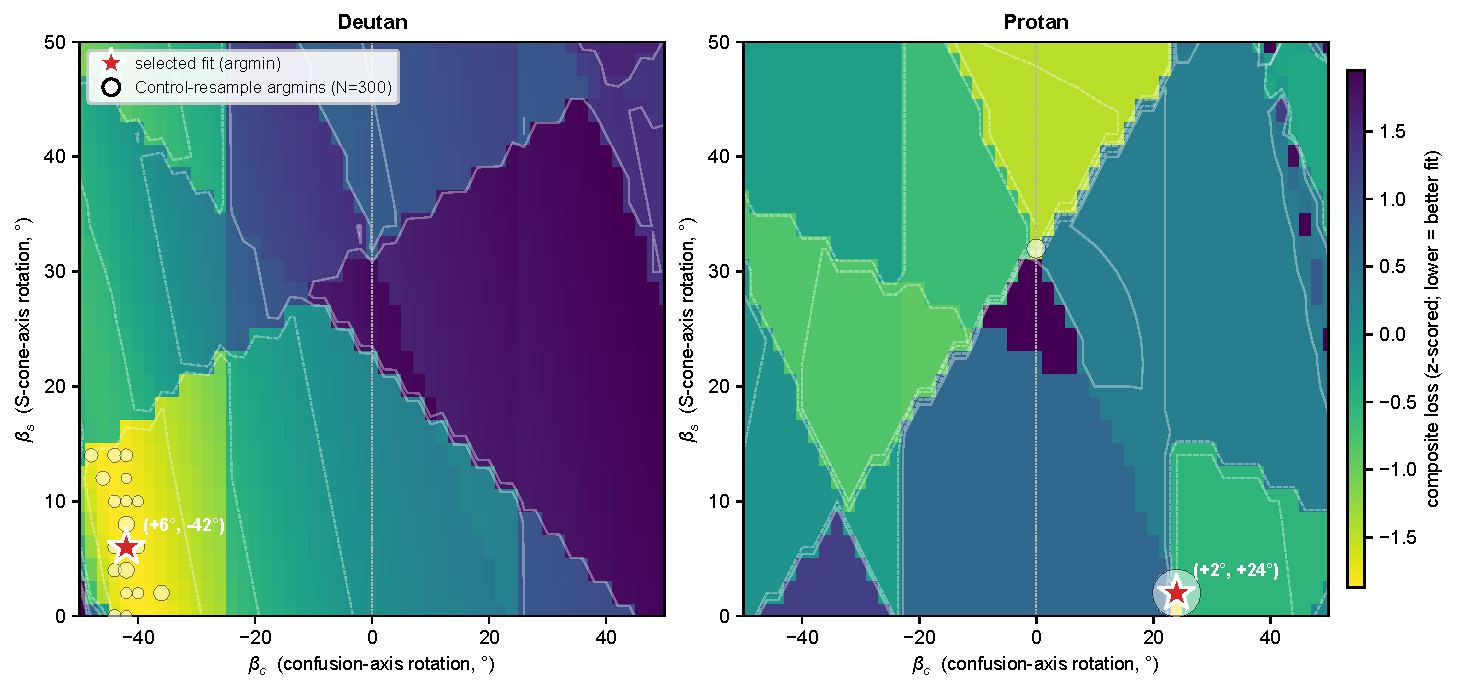
\includegraphics[width=\textwidth]{figS1_landscape}
  \caption{\textbf{Per-subject loss landscape and parameter uncertainty.}
  The $z$-scored composite loss over the $(\beta_s, \beta_c)$ grid, reconstructed on the full seven-control pool, with lower values in yellow.
  The loss combination is $\gamma_{\rm OY} + L_{\rm RDM}^{(V2)}$ for the deutan participant and $\gamma_{\rm all} + L_{\rm RDM}^{(V1)}$ for the protan participant.
  The red star marks the argmin of that surface, at $(\hat\beta_s, \hat\beta_c) = (6^\circ, -42^\circ)$ for the deutan participant and $(2^\circ, +24^\circ)$ for the protan participant.
  It is a descriptive low-dimensional embedding of the distortion rather than a physiological point estimate.
  White points give the per-resample argmins over $N = 300$ control 5-train/2-test resamples.}
  \label{fig:landscape}
\end{figure}


% --------------------------------------------------------------------------
% ==== S13  Stability of the selected fits ====
% --------------------------------------------------------------------------

\suppsection{Stability of the selected fits}{app:fit_stability}

\paragraph{Control leave-one-out magnitude anchor.}
Both CVD estimates fall inside the corresponding control range, so parameter magnitude alone is a descriptive anchor rather than a test of CVD-versus-control specificity. Each of the $n = 7$ control participants was refit as a pseudo-CVD case with the remaining control pool as reference, under that participant's own selected loss. The deutan combination is $\gamma_{\rm OY} + L_{\rm RDM}^{(V2)}$ and the protan combination $\gamma_{\rm all} + L_{\rm RDM}^{(V1)}$. The deutan estimate is $\|\hat\beta\| = 42.4^\circ$ against a control range of $30.5^\circ$ to $58.1^\circ$ (mean $49.1^\circ$). The protan estimate is $24.1^\circ$ against $23.4^\circ$ to $55.5^\circ$ (mean $35.7^\circ$), close to the lower bound.

\paragraph{Sign stability across the two preprocessing pipelines.}
Each participant's selected loss combination was refit on the head-motion-corrected pipeline (\cref{app:uncorrected}) with every other element of the procedure held fixed, and the two participants diverge. The sign of $\hat\beta_c$ held for the deutan participant, whose median moved from $-42^\circ$ to $-46^\circ$ with the fraction of negative resamples at $1.000$ and $0.947$. It reversed for the protan participant, whose median moved from $+24^\circ$ to $-12^\circ$, with the head-motion-corrected pipeline returning $79.3\%$ negative resamples against none under the primary pipeline. The deutan fit was also more poorly conditioned on the second pipeline, the combined fraction of resamples reaching a grid boundary rising from $0.09$ to $0.72$, and those boundary solutions lie on the same side as the median, so they bear on the magnitude rather than on the sign. The psychophysical atoms are independent of preprocessing, so the neural atom is the sole component that differs between the two fits. We therefore report the deployed protan parameter as a frozen value and give it no physiological interpretation.

\paragraph{Resample structure.}
Each participant's selected fit is the global minimum of its loss surface on the full data (\cref{fig:landscape}), and the $(32^\circ, 0^\circ)$ solution lies in the secondary basin of the protan PCA landscape, so the two reductions disagree about which basin is the minimum. Across the 300 resamples $\hat\beta_c$ concentrates at $-42^\circ$ and $-44^\circ$ ($202$ of $300$) and stays within $[-48^\circ, -36^\circ]$, whereas $\hat\beta_s$ is distributed almost uniformly from $0^\circ$ to $14^\circ$.

\paragraph{Gate statistics and neural-term ablation.}
Table~\ref{tab:fit_stability} collects the statistics that describe how each selected cell was reached and how stable it is. The separation block reports the precondition that admitted a $\Delta$RDM atom at a given ROI (\S\ref{sec:methods:selection}). The ablation block refits each participant's selected combination with the psychophysical atoms alone and with the $\Delta$RDM atom alone, holding every other element of the procedure fixed, so the three argmins are directly comparable. All entries are medians over the same $N = 300$ control 5-train/2-test resamples, on the PCA-basis loss unless the row names the SRM basis.

\begin{table}[htbp]
  \caption{Gate statistics, neural-term ablation, and resample stability for the two selected fits. Separation $d$ is the standardized distance between the participant and the control distribution at each ROI, and the $\Delta$RDM atom was admissible only where it was positive and exceeded the pre-set threshold (\S\ref{sec:methods:selection}), which left all four ROIs in the deutan participant and V1 alone in the protan participant. $\Delta\overline{L}$ is the change in an atom's held-out loss at the selected cell relative to the no-distortion cell $(0^\circ, 0^\circ)$, with negative values favoring the fitted distortion, and the fold count gives how many of the seven leave-one-out folds favor it. The boundary-saturation rate is the fraction of resamples whose solution reached a grid edge. Parameter IQRs are given as $(\beta_s, \beta_c)$.}
  \label{tab:fit_stability}
  \centering
  \small
  \begin{tabular}{lcc}
    \toprule
    & Deutan & Protan \\ \midrule
    \multicolumn{3}{l}{\emph{Separation precondition}} \\
    \quad $d$ at V1 / V2 / V3 / hV4 & $2.31$ / $1.94$ / $0.86$ / $2.19$ & $0.81$ / $-0.23$ / $-0.48$ / $-0.24$ \\
    \quad Loss combinations passing the gate & 25 & 4 \\ \midrule
    \multicolumn{3}{l}{\emph{Held-out generalization of the selected cell}} \\
    \quad Grid percentile & $4.6\%$ & $8.1\%$ \\
    \quad $\Delta\overline{L}$, psychophysical atom & $-13.85$ (5 of 7) & $+0.01$ (3 of 7) \\
    \quad $\Delta\overline{L}$, $\Delta$RDM atom & $-0.41$ (7 of 7) & $-0.47$ (7 of 7) \\ \midrule
    \multicolumn{3}{l}{\emph{Neural-term ablation (argmin)}} \\
    \quad Psychophysical atoms alone & $(16^\circ, -44^\circ)$ & $(26^\circ, +4^\circ)$ \\
    \quad $\Delta$RDM atom alone & $(4^\circ, -26^\circ)$ & $(0^\circ, +24^\circ)$ \\
    \quad Selected combination & $(6^\circ, -42^\circ)$ & $(2^\circ, +24^\circ)$ \\
    \quad Selected combination, SRM basis & $(8^\circ, -42^\circ)$ & $(32^\circ, 0^\circ)$ \\ \midrule
    \multicolumn{3}{l}{\emph{Resample stability, psychophysical alone $\rightarrow$ selected}} \\
    \quad Boundary-saturation rate & $0.23 \rightarrow 0.09$ & $0.00 \rightarrow 0.00$ \\
    \quad Parameter IQR, PCA basis & $(18^\circ, 6^\circ) \rightarrow (8^\circ, 2^\circ)$ & $(6^\circ, 4^\circ) \rightarrow (0^\circ, 0^\circ)$ \\
    \quad Parameter IQR, SRM basis & $(18^\circ, 6^\circ) \rightarrow (10^\circ, 4^\circ)$ & $(6^\circ, 4^\circ) \rightarrow (0^\circ, 2^\circ)$ \\
    \bottomrule
  \end{tabular}
\end{table}


\suppsection{Filter-evaluation session design and comparator}{app:filter_eval}

\paragraph{Comparator.}
The deployed comparator was the macOS accessibility Color Filter (System Settings $>$ Accessibility $>$ Display, build 26.5.1), set at an intensity the participant self-tuned before scanning. It is the unmodified shipping product, an operating-system-level post-display transform. We compared against it rather than a re-implemented retinal-simulation transform so that the comparator is the correction an end user actually encounters. The individualized filter was rendered directly in PsychoPy from the frozen per-subject pre-image.

\paragraph{Acquisition.}
Eight fMRI runs were acquired in ABBA-counterbalanced order, four per filter. Scanner time set this count, since six runs per condition would run roughly 90 minutes, beyond the 60--75-minute window over which participant attention and head motion stay acceptable. Four runs per condition take about 60 minutes, at the lower edge of that window.

\paragraph{Run-count adequacy.}
Four runs preserve the Session-1 separation between the control mean and the two CVD cases at hV4. Across all $\binom{6}{n}$ subsets of the six-run Session-1 data, hV4 LOCO adjacent accuracy held that separation at every run count down to four (\cref{fig:adjacc_saturation}). At $n = 4$ the control mean reached $0.45$ against $0.46$ at six runs and stayed above the $0.25$ chance level, while both CVD participants stayed below it (deutan $0.23$, protan $0.14$, single-case $d_{cc} < -2$ in both). Four runs nonetheless fall below the count recommended for fine-grained RDM-based model comparison, so the second session targets movement toward or away from the control reference rather than adjudication between model classes.

The filter conditions each have four runs, whereas the Session-1 control reference and the unfiltered baseline each have six. Noise in either pattern inflates disparity and RDM similarity, so an unmatched comparison would penalize the filter conditions twice, once against the baseline and once against the control distribution that the single-case test uses. Every neural index is therefore reported run-matched. For the interpolation indices the control reference is subsampled to four runs. For the geometry indices both the control means and the unfiltered baseline are rebuilt from four runs, exhaustively over all $\binom{6}{4} = 15$ subsets, with the shared response model refitted within each subset and the resulting metrics averaged (\texttt{exp2\_runmatched\_geometry.py}). The filter conditions themselves are never subsampled. The control reference comprises $n = 7$ controls at V1--V3 and $n = 6$ at hV4, where one control has too few voxels. Matching raises the protan V1 RDM similarity of the unfiltered baseline from $0.25$ to $0.33$, which places the individualized filter's value below that baseline rather than above it, and leaves the ordering of conditions unchanged on all four indices.
% TERMINOLOGY (resolved 2026-08-05): was "RDM-based model discrimination"; changed to
% "model comparison". "discrimination" is now reserved paper-wide for the behavioral
% JND construct; the neural LORO construct is "color classification".

\begin{figure}[tb]
  \renewcommand{\thefigure}{S\arabic{figure}}  % see the note on the first supplementary figure
  \centering
  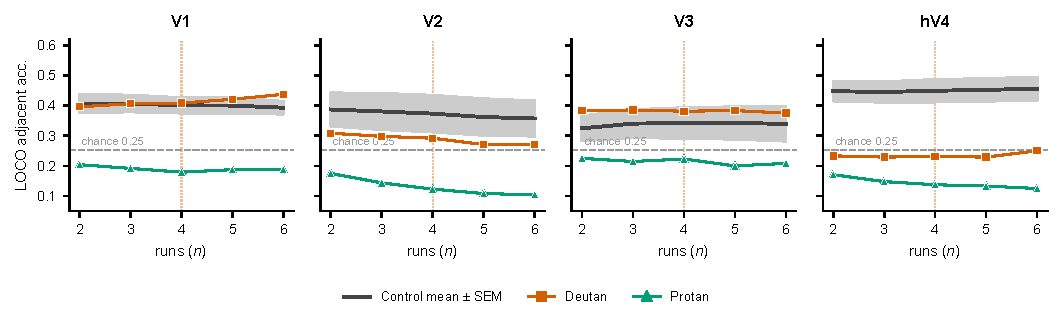
\includegraphics[width=\linewidth]{figS2_adjacc_saturation}
  \caption{\textbf{Hue-interpolation adjacent accuracy as a function of the number of runs.} LOCO adjacent accuracy (six-channel basis, OLS pseudoinverse decoder) as a function of the number of runs $n$, computed over all $\binom{6}{n}$ run subsets of the Session-1 data, per ROI. Black line, control mean $\pm$ SEM (shaded band); dashed line, the $0.25$ chance level; markers, the two CVD single cases (deutan, protan). The orange guide marks the deployed $n = 4$.}
  \label{fig:adjacc_saturation}
\end{figure}

\paragraph{Single-case inference.}
Each condition's neural index was compared to the control distribution as the case-control effect size $d_{cc}$ (\S\ref{sec:methods:stats}), reported in place of an inferential $p$ because the grand-mean permutation null is biased for this design. Robustness was assessed by leave-one-run separation, the contrast holding after any single run is dropped, and by re-extracting both conditions on the no-filter baseline voxel set.

% --------------------------------------------------------------------------
% ==== S15  Second-session outcomes by condition ====
% Split from the former "Filter-evaluation session design and comparator"
% on 2026-09-04: the design half and the condition-level results half each
% carry their own exhibits (words_trimming.md §5.4).
% --------------------------------------------------------------------------

\suppsection{Second-session outcomes by condition}{app:exp2_outcomes}

Each index below is reported for the unfiltered Session-1 baseline (NF), the deployed accessibility filter (Dep), and the individualized filter (Ind), run-matched as described in \cref{app:filter_eval}.

\paragraph{Hue identification (8AFC).}
Identification accuracy stayed at or above the Session-1 baseline under the individualized filter in both participants (\cref{tab:exp2_8afc}). This task entered neither fitting term, so it is a prospective test of the filters (\S\ref{sec:results:filter_eval}).

\begin{table}[tb]
  \centering
  \caption{\textbf{Second-session hue identification (8AFC).} Accuracy over $n = 64$ trials per cell with the 95\% Wilson score interval. Chance $= 0.125$. NF, no-filter (Session-1 baseline); Dep, deployed accessibility filter; Ind, individualized filter.}
  \label{tab:exp2_8afc}
  \begin{tabular}{llcc}
    \toprule
    Participant & Condition & Accuracy & 95\% CI \\
    \midrule
    Deutan & NF  & 0.81 & $[0.70, 0.89]$ \\
                    & Dep & 0.97 & $[0.89, 0.99]$ \\
                    & Ind & 0.97 & $[0.89, 0.99]$ \\
    \midrule
    Protan & NF  & 1.00 & $[0.94, 1.00]$ \\
                    & Dep & 0.86 & $[0.75, 0.92]$ \\
                    & Ind & 0.98 & $[0.92, 1.00]$ \\
    \bottomrule
  \end{tabular}
\end{table}

\paragraph{Hue classification (LORO).}
The displayed hues remained decodable under both filters (\cref{tab:exp2_loro}). Every cell stayed above the $0.125$ chance level. The lowest cell, $0.50$ at hV4 under the individualized filter in the deutan participant, lies below the control range of $0.71$ to $0.77$.

\begin{table}[tb]
  \centering
  \caption{\textbf{Second-session hue classification (LORO eight-way classification accuracy).} Chance $= 0.125$. NF, no-filter (Session-1 baseline); Dep, deployed accessibility filter; Ind, individualized filter. Controls, mean ($n = 7$).}
  \label{tab:exp2_loro}
  \begin{tabular}{lccccccc}
    \toprule
     & & \multicolumn{3}{c}{Deutan} & \multicolumn{3}{c}{Protan} \\
    \cmidrule(lr){3-5} \cmidrule(lr){6-8}
    ROI & Controls & NF & Dep & Ind & NF & Dep & Ind \\
    \midrule
    V1  & 0.71 & 0.79 & 0.84 & 0.72 & 0.79 & 0.91 & 0.66 \\
    V2  & 0.71 & 0.79 & 0.69 & 0.62 & 0.83 & 0.75 & 0.72 \\
    V3  & 0.77 & 0.67 & 0.78 & 0.69 & 0.81 & 1.00 & 0.69 \\
    hV4 & 0.75 & 0.73 & 0.88 & 0.50 & 0.71 & 0.84 & 0.69 \\
    \bottomrule
  \end{tabular}
\end{table}

\paragraph{Interpolation and geometry by condition.}
The three neural indices of the second session appear in \cref{tab:exp2_geometry} at each participant's target region, with the control reference and the single-case effect size for every condition.

\begin{table}[tb]
  \centering
  \caption{\textbf{Second-session interpolation and representational geometry.} All entries are run-matched (four runs per cell). NF, no-filter (Session-1 baseline); Dep, deployed accessibility filter; Ind, individualized filter. Parenthetical values are Crawford--Howell single-case effect sizes $d_{cc}$ against the control distribution. For adjacent accuracy the control entry is the mean $\pm$ SD over $n = 6$ controls at hV4 and the analytic chance level is $0.25$. For SRM disparity the control entry is the mean over $n = 7$ controls and lower values are more control-like. For RDM similarity the control entry is the leave-one-out self-consistency, a single value with no dispersion, so no effect size is defined and higher values are more control-like. The target region is the one at which each participant's Session-1 disparity was elevated, V2 for the deutan and V1 for the protan participant.}
  \label{tab:exp2_geometry}
  \small
  \begin{tabular}{lcccc}
    \toprule
    Index & Controls & NF & Dep & Ind \\
    \midrule
    \multicolumn{5}{l}{\emph{Deutan}} \\
    \quad hV4 adjacent accuracy & $0.46 \pm 0.11$ & $0.23$ ($-2.11$) & $0.25$ ($-1.94$) & $0.31$ ($-1.35$) \\
    \quad V2 SRM disparity & $0.44$ & $0.68$ ($2.69$) & $0.87$ ($4.93$) & $0.77$ ($3.73$) \\
    \quad V2 RDM similarity & $0.59$ & $0.42$ & $0.16$ & $0.05$ \\
    \midrule
    \multicolumn{5}{l}{\emph{Protan}} \\
    \quad hV4 adjacent accuracy & $0.46 \pm 0.11$ & $0.14$ ($-2.99$) & $0.19$ ($-2.52$) & $0.06$ ($-3.70$) \\
    \quad V1 SRM disparity & $0.43$ & $0.70$ ($3.92$) & $0.66$ ($3.29$) & $0.63$ ($2.84$) \\
    \quad V1 RDM similarity & $0.66$ & $0.33$ & $0.38$ & $0.26$ \\
    \bottomrule
  \end{tabular}
\end{table}

\paragraph{Forward-tuning encoding index.}
The forward-tuning correlation $\rho$ is the Pearson correlation between the predicted and the observed voxel pattern, averaged over the eight held-out hues. It indexes the encoding fit rather than the decoding accuracy on which the comparison rests. Figure~\ref{fig:forward_tuning} shows this index against the reference hue map, reported as corroboration only, since it lies outside the validated Session-1 decoding pipeline. In the deutan participant the individualized filter approaches the control level at hV4 ($\rho = +0.18$ against controls $+0.21$) while under the deployed filter it falls to $\rho = -0.39$. In the protan participant the three conditions do not separate, all reaching $\rho \approx -0.02$ at hV4.

\begin{figure}[tb]
  \renewcommand{\thefigure}{S\arabic{figure}}  % see note on the previous figure
  \centering
  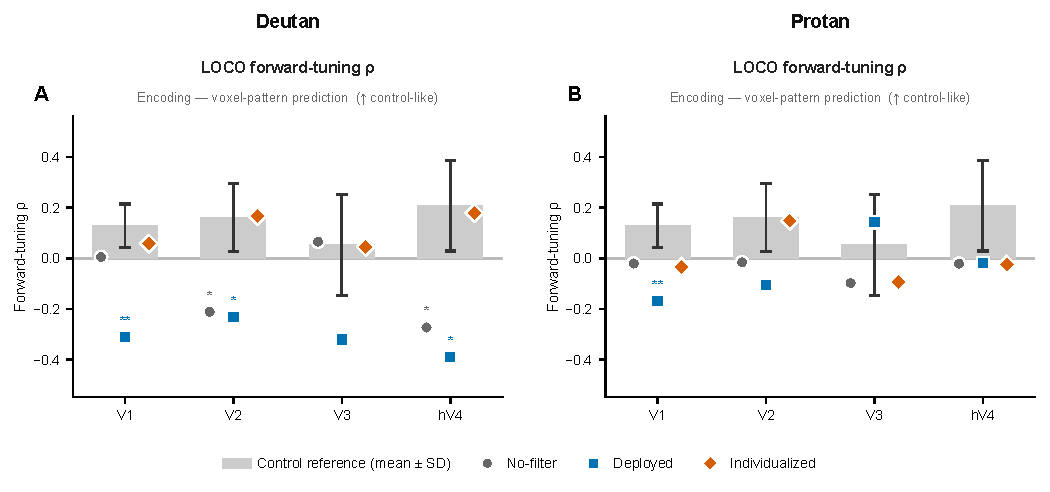
\includegraphics[width=\linewidth]{figS3_forward_tuning}
  \caption{\textbf{Forward-tuning encoding index (corroboration only).} LOCO forward-tuning correlation $\rho$ to the reference hue map across V1--hV4, for the deutan (left) and protan (right) participants ($\uparrow$ control-like). Gray bars, control reference (mean $\pm$ SD, $n = 7$); markers, no-filter (gray circle), deployed accessibility filter (blue square), individualized filter (orange diamond). Stars, Crawford--Howell single-case deviation from the control distribution ($^{*}p<.05$, $^{**}p<.01$).}
  \label{fig:forward_tuning}
\end{figure}


% ========== Section 14: Effect Sizes ==========

% --------------------------------------------------------------------------
% ==== S16  Statistical analysis and effect sizes ====
% Merger of the former "Effect sizes for single-case comparisons" and
% "Statistical analysis" sections (2026-09-04). The two defined d_cc in terms
% of each other; Methods §sec:methods:stats now points here once.
% The cross-subject encoder-transfer comparison moved to \cref{app:decoders},
% where it belongs with the decoder results (words_trimming.md §5.4).
% --------------------------------------------------------------------------

\suppsection{Statistical analysis and effect sizes}{app:statistics}

Unless noted otherwise, the significance threshold was $\alpha = 0.05$. False Discovery Rate correction \parencite{benjamini1995} was applied within two pre-specified families alone, the RDM hue-pair comparisons ($q = 0.05$, 28 pairs per participant) and the six parameter-identifiability checks (\cref{sec:methods:identifiability}). The exploratory per-hue vulnerability comparisons and the per-pair identification tests, including the blue-hue deficit, are reported one-tailed and uncorrected. Individual CVD participants were compared to the control distribution using the \textcite{crawford1998} modified $t$-test,

with the tail set by the pre-specified direction of each endpoint, one-tailed upper for disparity, one-tailed lower for interpolation, and two-tailed for classification and for the activation metrics.

Single-case effect sizes are the case-control index $d_{cc} = (x_{\rm case} - \bar{x}_{\rm ctrl}) / s_{\rm ctrl} = t\sqrt{(n+1)/n}$, where $n$ is the control sample size used in the test. Mann--Whitney $U$ tests use the rank-biserial correlation $r_{\rm rb}$ as their effect size, and group-level effect sizes are Hedges' $g$ \parencite{hedges1985}. Effect sizes for the single-case interpolation comparisons appear in \cref{tab:effect_sizes}, and the geometric-disparity effect sizes appear beside their $t$ statistics in \cref{tab:disparity_loso}. Single-case comparisons of within-subject LORO accuracy against the control distribution reached $|d_{cc}|$ between $0.25$ and $1.58$ across the eight participant-by-ROI tests, with all $p \geq 0.189$ (two-tailed). The largest deviation was the deutan participant at V3 ($d_{cc} = -1.58$), and at hV4 both participants gave $d_{cc} = -1.08$ ($p = 0.352$).

\begin{table}[h]
\centering
\caption{Effect sizes for the single-case hue-interpolation comparisons at hV4 (main text, \S\ref{sec:results:loco}). Crawford--Howell case-control effect size $d_{cc} = t\sqrt{(n+1)/n}$ against the $n = 7$ control distribution, one-tailed. Per-hue tests are uncorrected and exploratory across eight hues. Both CVD participants share identical statistics at the three hues where adjacent accuracy is zero. Blue lies just above the conventional threshold and is the largest per-hue deviation.}
\label{tab:effect_sizes}
\begin{tabular}{lccc}
\toprule
Comparison (hV4) & $t$ & $p$ & $d_{cc}$ \\
\midrule
LOCO adjacent accuracy, deutan & $-1.89$ & $0.054$ & $-2.02$ \\
LOCO adjacent accuracy, protan & $-3.04$ & $0.012$ & $-3.25$ \\
\midrule
\multicolumn{4}{l}{\emph{Per-hue adjacent accuracy (one-tailed, exploratory; both participants)}} \\
Blue & $-1.93$ & $0.051$ & $-2.06$ \\
Purple & $-0.79$ & $0.229$ & $-0.85$ \\
Magenta & $-1.47$ & $0.096$ & $-1.57$ \\
\bottomrule
\end{tabular}
\end{table}


\suppsection{Alignment robustness of the within-subject readouts}{app:alignment}

The two alignment spaces agree on the pattern on which the Results rest. LORO and LOCO are trained and tested within a single participant, so the main text computes them on the Procrustes-aligned amplitudes, which retain that participant's voxels at full resolution, and SRM enters only where a comparison spans participants. \cref{tab:alignment} gives both readouts in the Procrustes space, and the hue-channel-basis rows of \cref{tab:loro_decoders,tab:loco_decoders} give the same readouts in the SRM space.

Classification stays above the $0.125$ chance level for both CVD participants at every region in both spaces, with the lowest cell at $0.312$. Interpolation at hV4 remains reduced in both participants in both spaces, and the ordering of the two participants is preserved. Procrustes alignment yields the higher control-mean accuracy at all four regions for classification and at three of the four for interpolation, and it is the higher of the two spaces in 26 of the 36 participant-by-region classification cells. This follows from the dimensionality reduction in SRM discarding response variance that a within-subject readout can otherwise use.

The spaces differ at V1 classification, where SRM places both CVD participants above the control mean ($d_{cc} = +0.59$ and $+0.79$) while Procrustes places them slightly below ($d_{cc} = -0.25$ for both). Every single-case classification comparison stayed short of significance in both spaces.

\begin{table}[h]
\centering
\caption{Hue-channel basis readouts in the Procrustes-aligned space, which the main text reports. LORO is eight-way classification accuracy (chance $0.125$); LOCO is adjacent accuracy (analytic chance $0.25$). The control column is the mean over $n = 7$. The SRM-aligned counterpart of every cell appears in the forward-encoding rows of \cref{tab:loro_decoders,tab:loco_decoders}.}
\label{tab:alignment}
\begin{tabular}{lcccccc}
\toprule
& \multicolumn{3}{c}{LORO classification} & \multicolumn{3}{c}{LOCO interpolation} \\
\cmidrule(lr){2-4}\cmidrule(lr){5-7}
Region & Controls & deutan & protan & Controls & deutan & protan \\
\midrule
V1  & $0.580$ & $0.562$ & $0.562$ & $0.393$ & $0.437$ & $0.188$ \\
V2  & $0.607$ & $0.521$ & $0.562$ & $0.357$ & $0.271$ & $0.104$ \\
V3  & $0.574$ & $0.396$ & $0.458$ & $0.339$ & $0.375$ & $0.208$ \\
hV4 & $0.488$ & $0.375$ & $0.375$ & $0.456$ & $0.250$ & $0.125$ \\
\bottomrule
\end{tabular}
\end{table}


% --------------------------------------------------------------------------
% ==== S17  (was Supplementary/S18_geometry_validity.tex) ====
% --------------------------------------------------------------------------
% Supplementary S16 — Validity of the geometric comparison
% 2026-08-07
% Governing document: docs/PAPER/REVISION_PLAN_MOTION_GEOMETRY_2026-08-06.md §S18 (rule R5).
% Source numbers: analysis/phase2_SRM_across_between/results/RESULTS_GEOMETRY_VALIDITY_2026-08-05.md
%   §1 (control positive control), §2 (color specificity), §4 (cyclic shift)
% Raw outputs: analysis/future_phase1_sensitivity/results/{with_residuals,hmc_v2}/color_correspondence/frozen_permutation.json,
%   analysis/validation/results/cyclic_shift_disparity.json (hmc_v2 variant not yet computed)
% Counts and BH-FDR recomputed from the JSON on 2026-08-07:
%   35 cells, 16 raw p<.05 (the "15" in RESULTS_GEOMETRY_VALIDITY §2 prose is a
%   miscount of its own table), 7 surviving BH; motion-regressed 18 raw / 15 BH.
% The cyclic-shift gain is referred to the control gain distribution, which is computed
%   under the same minimum-over-eight rule and therefore absorbs the same selection
%   bias. hV4 shift gains are omitted: the ROI carries no geometric endpoint, and
%   the motion-regressed control gain SD there collapses to 0.38%.

\suppsection{Validity of the geometric comparison}{app:geometry_validity}

The color-correspondence permutation has power only when the shared projection is held fixed, since re-estimating it at each permutation allows the re-fit to absorb the permutation. The permutation asks whether a participant's colors map onto the control geometry in the identity order, which differs from the color-label permutation null of the main text, where the question is whether the control group interpolates above chance in a region. We tested both variants on the controls, in whom color structure is established. Re-estimation detected 0 of 7 at V1, V2 and V3 and 0 of 6 at hV4, with mean permutation $z$ near zero in every ROI, whereas freezing the projection recovered detection, reaching 5 of 7 at V3 and 2 to 3 of 7 elsewhere (\cref{tab:frozen_control}). Every color-specificity result below uses the frozen projection.

\begin{table}[h]
\centering
\caption{Color-correspondence permutation on the controls, used as a positive control. Detection counts and mean permutation $z$ under a projection re-estimated at each permutation and under a frozen projection. Lower $z$ indicates a better identity correspondence than the shuffled null.}
\label{tab:frozen_control}
\begin{tabular}{lccccc}
\toprule
 & & \multicolumn{2}{c}{Re-estimated} & \multicolumn{2}{c}{Frozen} \\
\cmidrule(lr){3-4}\cmidrule(lr){5-6}
ROI & $n$ & detected & mean $z$ & detected & mean $z$ \\
\midrule
V1  & 7 & 0 & $-0.04$ & 2 & $-1.58$ \\
V2  & 7 & 0 & $-0.04$ & 3 & $-1.00$ \\
V3  & 7 & 0 & $-0.78$ & 5 & $-2.39$ \\
hV4 & 6 & 0 & $+0.06$ & 2 & $-1.07$ \\
\bottomrule
\end{tabular}
\end{table}

Both CVD participants showed color-specific geometry. The deutan participant reached $p = .002$ at V2, the lowest V2 value among the nine participants, and $p = .024$ at V3. The protan participant reached $p = .001$ at V3 and $p = .013$ at V2, while V1 returned $p = .758$. Across the 35 participant-by-ROI cells, 16 fell below $.05$ against a chance expectation of $1.8$, and 7 survived Benjamini--Hochberg correction over all 35 (\cref{tab:color_specificity}). Two of the survivors belong to the CVD participants, the deutan V2 cell ($q = .018$) and the protan V3 cell ($q = .012$). V3 showed color specificity most broadly, with 5 of its 9 cells surviving.

\begin{table}[h]
\centering
\caption{Color-correspondence permutation under the frozen projection, one cell per participant and region, in the two preprocessing pipelines. Entries give $p_{\rm perm}$ against $N = 1{,}000$ permutations. Seven cells survive Benjamini--Hochberg correction across the 35 cells of the primary pipeline and none survive it in the head-motion-corrected pipeline.}
\label{tab:color_specificity}
\begin{tabular}{lcccccccc}
\toprule
 & \multicolumn{4}{c}{Primary} & \multicolumn{4}{c}{Head-motion correction} \\
\cmidrule(lr){2-5}\cmidrule(lr){6-9}
Participant & V1 & V2 & V3 & hV4 & V1 & V2 & V3 & hV4 \\
\midrule
Control 1 & $0.088$ & $0.020$ & $0.062$ & $0.393$ & $0.012$ & $0.072$ & $0.018$ & $0.290$ \\
Control 2 & $0.001$ & $0.016$ & $0.004$ & $0.136$ & $0.437$ & $0.420$ & $0.191$ & $0.019$ \\
Control 3 & $0.109$ & $0.520$ & $0.255$ & $0.272$ & $0.325$ & $0.113$ & $0.176$ & $0.101$ \\
Control 4 & $0.152$ & $0.014$ & $0.001$ & $0.041$ & $0.420$ & $0.006$ & $0.015$ & $0.173$ \\
Control 5 & $0.057$ & $0.773$ & $0.034$ & $0.031$ & $0.079$ & $0.194$ & $0.032$ & $0.038$ \\
Control 6 & $0.407$ & $0.290$ & $0.009$ & $0.220$ & $0.373$ & $0.117$ & $0.010$ & $0.012$ \\
Control 7 & $0.034$ & $0.159$ & $0.004$ & --- & $0.008$ & $0.005$ & $0.391$ & --- \\
\textbf{Deutan} & $0.105$ & $0.002$ & $0.024$ & $0.273$ & $0.022$ & $0.003$ & $0.047$ & $0.257$ \\
\textbf{Protan} & $0.758$ & $0.013$ & $0.001$ & $0.129$ & $0.010$ & $0.148$ & $0.053$ & $0.815$ \\
\bottomrule
\end{tabular}
\end{table}

Under head-motion correction 15 cells fell below $.05$ and none survived correction. The deutan V2 cell remained at its nominal value across the two pipelines ($p = .002$ and $p = .003$) while its corrected value moved from $q = .018$ to $q = .053$, and the protan V1 cell moved from $p = .758$ to $p = .010$. Individual cells of this grid are descriptive and support no claim in the main text.

The protan participant's V1 correspondence is displaced by one hue step, and the failure is not one of signal. That participant's V1 split-half pattern reliability reaches $.847$, above the highest control value, and eight-way classification there reaches $0.79$ against a chance level of $0.125$. Rotating the color labels by $45^\circ$ lowered Procrustes disparity from $1.037$ to $0.788$, a gain of $24.0\%$. We referred that gain to the distribution of shift gains across the seven controls ($3.5 \pm 5.9\%$), which is computed under the same minimum-over-eight rule and is therefore subject to the same selection bias. The protan gain exceeded that distribution (Crawford--Howell $t = 3.22$, $p = .009$, $d_{cc} = 3.44$), and the rotated geometry sat below the control mean disparity of $0.839 \pm 0.087$. The same rotation raised the second-order RSA similarity from $\rho \approx 0.00$ to $\rho = +0.52$, against a control mean of $0.45$, exceeding its own selection-bias null ($z = +5.02$, $p = .002$, $p_{\rm adj} = .032$). Disparity at this region is nonetheless elevated in both pipelines, so the departure is not accounted for by a rigid relabeling alone. The account applies to the primary pipeline, since that cell is no longer null under head-motion correction. The deutan participant showed the identity mapping as optimal at V1, V2 and V3.

Which rearrangement restores control-level similarity remains open. Under the SRM basis a $225^\circ$ shift ($+0.50$) is close to the $315^\circ$ optimum ($+0.52$). Under the PCA basis the optimum falls at $135^\circ$ ($p = .048$, which does not survive correction).
% Superseded sources: docs/PAPER/Supplementary/archive/ (gitignored)
% ============================================================================

\renewcommand{\thetable}{S\arabic{table}}\setcounter{table}{0}


% ========== Section 1: Session-1 hue-discrimination thresholds ==========

\suppsection{Session-1 hue-discrimination thresholds}{app:jnd_baseline}

Session-1 threshold elevations followed each participant's subtype (\cref{tab:jnd_baseline}). The threshold is the staircase level $t$, the fraction of the pair's full CIE $LCh$ separation at which the two discs were discriminated (\S\ref{sec:methods:psychophysical}), so smaller values indicate finer discrimination. The ratio $\gamma$ divides the participant's threshold by the control mean, and $z$ expresses the same difference in control standard deviations over the seven controls. Pairs are grouped by the axis each was chosen to probe, and that assignment was fixed before any threshold was collected.

Each pair was measured by two interleaved staircases from starting levels $t = 0.8$ and $t = 0.5$, both following a 1-up/1-down rule with a step of $0.15$ until the second reversal and $0.03$ thereafter. A staircase terminated at eight reversals and at least 20 trials, extended by two further reversals whenever the SD of the last six reversal levels exceeded $0.10$.

Elevation localized to the axis each participant's subtype predicts. The deutan participant exceeded $z = +4$ on both deutan-axis pairs and on the yellow--purple S-cone pair, and the protan participant exceeded the control range on the protan-axis pair green--blue alone. Both participants remained inside the control range on the $180^\circ$ control pair, which places the elevation on specific axes rather than on overall sensitivity. These thresholds enter the psychophysical loss atoms of \S\ref{sec:methods:candidates}, and the same eight pairs supply the pre-filter baseline of the filter evaluation (\S\ref{sec:results:filter_eval}).

\begin{table}[h]
\centering
\caption{Session-1 hue-discrimination thresholds without a filter. The control column is the mean $\pm$ SD over the seven controls. $\gamma$ is the ratio to the control mean and $z$ the deviation in control standard deviations. Bold: $|z| \geq 2$. Two staircases returned an incorrect response at the largest presentable separation, both of them the deutan participant's orange--yellow pair, so that threshold is a lower bound rather than an estimate. It is the only such pair among the 208 staircases collected in this study.}
\label{tab:jnd_baseline}
\setlength{\tabcolsep}{4pt}
\begin{tabular}{llcccccccc}
\toprule
& & \multicolumn{2}{c}{Controls ($n = 7$)} & \multicolumn{3}{c}{Deutan} & \multicolumn{3}{c}{Protan} \\
\cmidrule(lr){3-4}\cmidrule(lr){5-7}\cmidrule(lr){8-10}
Axis probed & Pair & mean & SD & $t$ & $\gamma$ & $z$ & $t$ & $\gamma$ & $z$ \\
\midrule
Deutan confusion & orange--yellow & $0.278$ & $0.135$ & $0.840$ & $\mathbf{3.02}$ & $\mathbf{+4.15}$ & $0.193$ & $0.69$ & $-0.63$ \\
                 & yellow--green  & $0.090$ & $0.044$ & $0.278$ & $\mathbf{3.10}$ & $\mathbf{+4.32}$ & $0.128$ & $1.42$ & $+0.87$ \\
\midrule
Protan confusion & green--blue    & $0.079$ & $0.032$ & $0.078$ & $0.98$ & $-0.06$ & $0.155$ & $\mathbf{1.95}$ & $\mathbf{+2.36}$ \\
                 & cyan--magenta  & $0.042$ & $0.017$ & $0.040$ & $0.95$ & $-0.13$ & $0.038$ & $0.89$ & $-0.28$ \\
\midrule
S-cone           & yellow--purple & $0.022$ & $0.006$ & $0.063$ & $\mathbf{2.87}$ & $\mathbf{+6.70}$ & $0.028$ & $1.26$ & $+0.94$ \\
                 & blue--purple   & $0.164$ & $0.093$ & $0.120$ & $0.73$ & $-0.48$ & $0.148$ & $0.90$ & $-0.18$ \\
                 & red--orange    & $0.124$ & $0.072$ & $0.063$ & $0.50$ & $-0.85$ & $0.075$ & $0.61$ & $-0.68$ \\
\midrule
Control          & red--cyan      & $0.034$ & $0.015$ & $0.015$ & $0.45$ & $-1.23$ & $0.015$ & $0.45$ & $-1.23$ \\
\midrule
\multicolumn{7}{l}{Mean $|z|$ over the eight pairs \quad Deutan $2.24$ \quad Protan $0.90$} & & & \\
\bottomrule
\end{tabular}
\end{table}


The deutan orange--yellow threshold is a lower bound. Both of its staircases remained at the top of the presented range throughout and returned incorrect responses at the largest separation the task presents. Censoring understates the baseline deficit and therefore the improvement recorded under either filter, so the value is reported unadjusted.

\begin{table}[h]\centering\small
\caption{Both staircase estimates for every hue pair, given as high-start/low-start in units of the rendered separation. Bold marks the cells whose two estimates differ by more than 0.10. Thresholds reported elsewhere are the mean of the two.}
\label{tab:staircase_pairs}
\begin{tabular}{lcccccc}
\toprule
 & \multicolumn{3}{c}{Deutan} & \multicolumn{3}{c}{Protan} \\
\cmidrule(lr){2-4}\cmidrule(lr){5-7}
Pair & Session 1 & Deployed & Individualized & Session 1 & Deployed & Individualized \\
\midrule
red--orange & 0.060/0.065 & 0.160/0.210 & 0.140/0.130 & 0.075/0.075 & 0.110/0.145 & 0.070/0.055 \\
orange--yellow & 0.870/0.810 & 0.080/0.110 & 0.060/0.032 & 0.175/0.210 & 0.170/0.185 & \textbf{0.715/0.200} \\
yellow--green & 0.280/0.275 & 0.090/0.075 & 0.145/0.165 & 0.125/0.130 & 0.057/0.050 & 0.055/0.065 \\
green--blue & 0.065/0.090 & 0.150/0.110 & 0.045/0.060 & 0.145/0.165 & 0.260/0.225 & 0.135/0.080 \\
blue--purple & 0.115/0.125 & 0.050/0.095 & 0.110/0.200 & 0.125/0.170 & 0.135/0.110 & 0.150/0.105 \\
yellow--purple & 0.060/0.065 & 0.015/0.020 & 0.035/0.025 & 0.020/0.035 & 0.020/0.015 & 0.015/0.015 \\
red--cyan & 0.015/0.015 & 0.040/0.018 & 0.015/0.045 & 0.015/0.015 & 0.030/0.040 & 0.020/0.025 \\
cyan--magenta & 0.035/0.045 & 0.030/0.025 & 0.040/0.033 & 0.040/0.035 & 0.150/0.140 & 0.015/0.020 \\
\bottomrule\end{tabular}\end{table}

The two staircases of a pair agreed closely (\cref{tab:staircase_pairs}). They differed by a median of $0.015$ across the $104$ pairs, and three cells exceeded $0.10$. The largest, at $0.515$, is the protan participant's orange--yellow pair under the individualized filter, where one track settled at $0.715$ after answering correctly at a four-fold smaller separation earlier in the same block while its partner converged at $0.200$ on the same rendered stimuli. We attribute that cell to a single lapse and report every threshold as the unadjusted mean of the two tracks. Restricting it to the converged track would move the cell from $z = +1.33$ to $z = -0.58$ and the participant's mean $|z|$ from $0.93$ to $0.84$.



% --------------------------------------------------------------------------
% ==== Sections carrying a "% ========== Section N ==========" banner below
%      (was Methods/supplementary_content.tex, archived) ====
% --------------------------------------------------------------------------
% Supplementary Methods - Content Only
% To be included via \input{Methods/supplementary_content}


% --------------------------------------------------------------------------
% ==== S2  (was Supplementary/S17_uncorrected_artifacts.tex) ====
% --------------------------------------------------------------------------
% Supplementary S1 — Preprocessing pipelines and sensitivity analyses
% 2026-08-07
% Scope: slice timing, head motion, susceptibility distortion were all left
%   uncorrected in the analyzed pipeline. Motion has a sensitivity analysis;
%   distortion and coregistration are argued on structural grounds.
% Source numbers: analysis/phase2_SRM_across_between/results/RESULTS_MOTION_ARMS_2026-08-05.md
%   Coregistration stability: docs/PAPER/METHODS_REVISION_STATUS_2026-08-07.md §3

\suppsection{Preprocessing pipelines and sensitivity analyses}{app:uncorrected}

\paragraph{The two pipelines.}
Every neural endpoint of the first session was computed under two pipelines. The primary pipeline resampled each functional volume once by a transform identical for every volume in a run. The second composed each volume's MCFLIRT rigid-body realignment matrix with that transform before the same single resampling, so the two differ in the alignment method and share the number of resamplings. Head-motion correction lowered ROI temporal signal-to-noise ratio by $1.7$ to $2.7\%$. In both, the per-run linear and constant drift terms of the general linear model constituted the entire nuisance model, and both pipelines left slice timing, susceptibility distortion, and temporal filtering out. Within-run motion was estimated by registering every volume to its run's middle volume and summarized as framewise displacement \parencite{power2012}, with rotations converted to displacement on a 50\,mm sphere. Across the nine analyzed participants mean framewise displacement reached $0.318 \pm 0.044$\,mm (controls $0.313 \pm 0.042$, CVD $0.338 \pm 0.046$), and $16.2\%$ of volumes exceeded $0.5$\,mm.

\paragraph{Disparity under the two pipelines.}
The regional attribution of disparity depends on the pipeline (\cref{tab:motion_arms}). Procrustes disparity was recomputed under head-motion correction with every other element held fixed. The protan V1 elevation remained the largest deviation in that participant under both pipelines and weakened from $p = .007$ to $p = .077$. In the deutan participant the largest deviation moved from V2 to V1 and the V2 value reversed in sign. Under the leave-one-subject-out estimator the protan V1 cell of the primary pipeline reached significance alone.

\begin{table}[h]
\centering
\caption{Procrustes disparity by participant and region under head-motion correction. Entries give the Crawford--Howell one-tailed $t$ with $p$ in parentheses, against the control leave-one-out distribution ($n = 7$), for the common-space estimator and for the leave-one-subject-out estimator on which the inference rests. The primary pipeline appears in \cref{tab:disparity_loso}, which adds the case-control effect sizes. Individual cells of this grid are descriptive and support no claim in the main text.}
\label{tab:motion_arms}
\small
\begin{tabular}{llcc}
\toprule
Participant & Region & Crawford--Howell & Leave-one-subject-out \\
\midrule
Deutan & V1  & $2.4$ ($.027$) & $1.6$ ($.080$) \\
Deutan & V2  & $-1.0$ ($.825$) & $-0.6$ ($.723$) \\
Deutan & V3  & $0.6$ ($.293$) & $0.4$ ($.338$) \\
Deutan & hV4 & $0.4$ ($.351$) & $0.4$ ($.356$) \\
Protan & V1  & $1.6$ ($.077$) & $1.3$ ($.121$) \\
Protan & V2  & $1.0$ ($.186$) & $0.1$ ($.480$) \\
Protan & V3  & $1.1$ ($.151$) & $1.0$ ($.178$) \\
Protan & hV4 & $1.4$ ($.101$) & $1.1$ ($.159$) \\
\bottomrule
\end{tabular}
\end{table}

\paragraph{Classification and interpolation under the two pipelines.}
The two readouts dissociate under both pipelines (\cref{tab:interp_arms}). The control-group interpolation gate, the two single-case comparisons at hV4 (\S\ref{sec:results:loco}), and the eight-way classification readout (\S\ref{sec:results:loro}) were recomputed the same way. hV4 alone passes the control gate in both pipelines, and both participants remain below the control mean in both. Classification survives in both. The lowest CVD cell across the four regions reaches $0.375$ under the primary pipeline and $0.229$ under head-motion correction, $1.8$ times the $0.125$ chance level. Every single-case classification contrast stayed above $p = .10$ in both pipelines, and the single-case interpolation contrasts reached significance under the primary pipeline alone.

\begin{table}[h]
\centering
\caption{Hue-interpolation adjacent accuracy and eight-way classification accuracy under the two pipelines. Upper rows give the control interpolation mean with its $p$ against $1{,}000$ per-subject color-label permutations ($n = 7$; the permutation null mean is $0.35$ in both pipelines). Middle rows give each CVD participant's interpolation accuracy at hV4 with the one-tailed Crawford--Howell $p$ against the control distribution. Lower rows give classification accuracy at hV4, for which chance is $0.125$ and the Crawford--Howell test is two-tailed because the hypothesis is preservation; the control mean is listed for reference and is not tested. The primary-pipeline accuracies appear with their full four-region grid in \cref{tab:alignment}. Individual cells of this grid are descriptive and support no claim in the main text.}
\label{tab:interp_arms}
\begin{tabular}{lcccc}
\toprule
 & \multicolumn{2}{c}{Primary} & \multicolumn{2}{c}{Head-motion correction} \\
\cmidrule(lr){2-3}\cmidrule(lr){4-5}
 & Accuracy & $p$ & Accuracy & $p$ \\
\midrule
\multicolumn{5}{l}{\emph{Interpolation (LOCO adjacent accuracy)}} \\
Controls V1  & $0.393$ & $.164$ & $0.283$ & $.922$ \\
Controls V2  & $0.357$ & $.424$ & $0.381$ & $.228$ \\
Controls V3  & $0.339$ & $.586$ & $0.315$ & $.810$ \\
Controls hV4 & $0.456$ & $.011$ & $0.451$ & $.023$ \\
Deutan hV4 & $0.250$ & $.054$ & $0.354$ & $.242$ \\
Protan hV4 & $0.125$ & $.012$ & $0.271$ & $.108$ \\
\midrule
\multicolumn{5}{l}{\emph{Classification (LORO eight-way accuracy)}} \\
Controls hV4 & $0.488$ & --- & $0.569$ & --- \\
Deutan hV4 & $0.375$ & $.351$ & $0.583$ & $.905$ \\
Protan hV4 & $0.375$ & $.351$ & $0.396$ & $.197$ \\
\bottomrule
\end{tabular}
\end{table}

\paragraph{Session-2 endpoints under the harmonized arm.}
The second-session cortical readouts depend on the preprocessing arm, so we report both arms and treat every directional contrast in them as provisional. The session was reprocessed with the anatomical images harmonized to the first and with head-motion correction, and the fourteen pre-specified endpoints were recomputed within each arm, so the control reference and the Session-1 unfiltered anchor always come from the same reconstruction. The control reference moved from $0.456$ to $0.445$ in hV4 adjacent accuracy, whereas the single-participant, single-condition cells moved far more. Eight of the ten directional contrasts defined on the native voxel mask reversed between arms, as did five of the ten defined on the run-matched mask. The geometry indices moved less, and the four contrasts at the pre-specified target regions held in both arms. The psychophysical endpoints are independent of preprocessing and are unchanged.

\paragraph{Susceptibility distortion.}
Susceptibility distortion within the analyzed ROIs is predominantly subvoxel and spatially smooth, which places it outside the set of explanations for the observed differences in representational geometry across hue conditions. A gradient-echo field map was acquired in each session and linked to the functional runs through the BIDS \texttt{IntendedFor} field, and both pipelines left it unconsumed, so the data retain distortion along the right--left phase-encoding direction. Field-map-derived mean displacement within each analyzed ROI ranged from $0.01$ to $0.76$ voxels ($0.02$--$1.52$\,mm) across the nine participants. Within-ROI spatial variation is the component that distorts a pattern rather than translating it, and it reached $0.05$--$0.21$ voxels in eight participants and $0.38$ voxels ($0.76$\,mm) in the ninth. The residual cost is spatial, reducing the precision with which atlas-defined regions are assigned to functional voxels.

\paragraph{Registration.}
The functional series cover occipital cortex alone, so registration used mutual information initialized from the scanner-defined obliquity in the NIfTI header, which tolerates limited coverage and requires no white-matter boundary. Two standard routes were evaluated first and both were rejected. A container-based route through fMRIPrep failed at the coregistration stage on every attempt with these partial-coverage series. Boundary-based registration within the custom pipeline snapped the functional slab onto an incorrect tissue boundary on visual inspection, an error on the order of $10$\,mm, where the mutual-information solution stayed within about $1$\,mm of the visually verified position. Whole-brain overlap indices favor boundary-based registration on these data, but Dice and ROI-coverage measures respond to the extent of overlap rather than to the position of a partial slab within the brain, so the choice rests on the visual criterion.

The mutual-information optimum is shallow under this field of view. Across the runs of a single session, where the fitted transform should be identical, the mean pairwise displacement of the solution ranged from $0.9$ to $4.2$\,mm. Removing facial voxels from the anatomical image, which leaves the brain unchanged, moved the solution by $1.9$\,mm in the deutan participant and $9.4$\,mm in the protan participant. The transform is fixed within a run, so it enters the eight hues of a run as run-to-run noise alone, which is attenuated by averaging over the six runs. Rigid-body estimation and distortion correction are constrained just as weakly when little of the head is imaged, so acquisitions of this type would benefit from correction validated for partial coverage.


% ========== Section 3: Quality Control ==========

\suppsection{ROI coverage}{app:roi_coverage}

ROI coverage averaged $83.5\%$ (SD $22.7\%$) across the nine analyzed participants, and $99.5\%$ of ROI voxels showed reliable stimulus-evoked responses. Coverage was computed as the intersection of the Wang atlas ROIs (V1, V2, V3, hV4) with each participant's BOLD brain mask in MNI space, taken per participant as the mean over the four regions and six runs. Its lowest value in the sample was $30.8\%$. Every analyzed participant entered the downstream analyses.


% ========== Section 4: K-Selection ==========

\suppsection{Dimensionality selection for the shared response model}{app:dimensionality}

SRM used $k = 4$ at V1 and V2 and $k = 3$ at V3 and hV4, with cross-subject RDM Spearman correlations of $0.60$, $0.57$, $0.55$ and $0.32$. The reduced dimension was determined by leave-one-subject-out cross-validation over the candidate values 2 to 6 \parencite{cunningham2014}. On each of the seven folds, one control participant was withheld from SRM training and three quality metrics were computed for every candidate. RDM split-half reliability was the Spearman correlation between representational dissimilarity matrices built from the odd runs 1, 3, and 5 and the even runs 2, 4, and 6 of the withheld participant in SRM space. The remaining two metrics were the cross-subject RDM correlation and the reconstruction error. Candidates were ranked within each fold and metric, and the candidate with the best mean rank was selected.


% --------------------------------------------------------------------------
% ==== S5  Alternative decoders ====
% --------------------------------------------------------------------------
% Supplementary S4 — Decoder comparison
% 2026-08-07. Resolves the dangling "Appendix A" reference at methods_v2.tex:149.
% Source (all committed JSON, dataset token C010):
%   LORO  analysis/phase3_decoder_comparing/results/loro/srm/sub-{01..09}_performance_raw.json
%         results.{ROI}.{model}[fold].acc_exact, averaged over the six folds
%   LOCO  analysis/phase3_decoder_comparing/results/loco/srm/sub-{01..09}_loco.json
%         results.{ROI}.{model}.overall_adjacent_acc
%   config models: LDA, Ridge, KernelRidge, SVM, MLP, ForwardEncoding; rois V1 V2 V3 V4;
%   K recovered from amplitudes_srm.npy shapes (V1 4, V2 4, V3 3, hV4 3) since dim_k is null.
% Provenance of the correlation readout: present in the repo at b3ce74d (2026-01-27),
%   plan document 1634142 (2026-02-17); the LOCO run is 2026-02-22 and LORO 2026-02-26.
%   It was therefore inherited and then verified, NOT selected by this comparison.
% Deliberately excluded: FE_PopVec / FE_RidgeEnc / FE_GaussML / FE_RidgeReg vary the
%   readout rather than the decoder and have no committed numeric output; the ensemble
%   variants were retired at 3ec8e51 / a825a7d (2026-02-26); HybridMLP / HybridSVR ran
%   for LOCO only and so cannot be placed beside the LORO table.

\suppsection{Comparison with alternative decoders}{app:decoders}

The hue-channel basis model was adopted for its interpolation behavior rather than for its classification accuracy. We compared six decoders on the same SRM-aligned amplitudes under both cross-validation schemes, which separate them in opposite directions. The present analyses rest on the interpolation result.

Linear discriminant analysis classified held-out runs most accurately at every ROI (\cref{tab:loro_decoders}). Its control mean reached $0.878$ at V1 against a chance level of $0.125$, with the support vector machine next at $0.777$ and the hue-channel basis model at $0.542$. The ordering held at V2, V3 and hV4. Four of the six decoders exceeded chance at every ROI, so eight-way classification is recoverable by several readouts and favors none of them.

Interpolation to a held-out hue reverses the ordering at hV4, the ROI on which the main analyses rest (\cref{tab:loco_decoders}). The hue-channel basis model reached an adjacent accuracy of $0.470$ there, against a chance level of $0.25$ for its continuous-hue output. It is the only decoder whose control mean exceeds its own chance level, doing so at V1 ($0.360$), V2 ($0.283$) and hV4, with the widest margin at hV4. The classifiers remained below their $0.375$ chance level at every ROI, and ridge and kernel ridge remained below $0.25$ everywhere. The analytic chance level compares a decoder against a uniform prediction, whereas the stricter main-text criterion uses a color-label permutation null that preserves the covariance among voxels, and hV4 is the region that meets it (\S\ref{sec:results:loco}). The pattern follows from the model form. The hue-channel basis model represents a hue as activation over six tuned channels and can therefore evaluate a hue it never saw during training, whereas a classifier trained on seven discrete labels has no output unit for the eighth.

Two decoders produced constant outputs. Kernel ridge regression returned an adjacent accuracy of exactly $0.000$ in every participant, ROI and alignment, and the multilayer perceptron returned exactly the chance value with zero variance across participants, which is the signature of a constant prediction. We treat both as uninformative rather than competitive.

\begin{table}[h]
\centering
\caption{Eight-way classification accuracy under leave-one-run-out cross-validation, SRM-aligned amplitudes, chance $= 0.125$. control mean $\pm$ SD ($n = 7$), with the two CVD participants listed separately. Bold: highest control mean in the ROI. Three further variants sit outside this comparison: the ensemble decoders were retired from the pipeline, the two hybrid decoders were run for interpolation alone, and four alternative readouts of the hue-channel basis model vary the readout rather than the decoder.}
\label{tab:loro_decoders}
\begin{tabular}{llccc}
\toprule
ROI & Decoder & Controls (mean $\pm$ SD) & Deutan & Protan \\
\midrule
V1 & LDA & $\mathbf{0.878 \pm 0.050}$ & 1.000 & 0.854 \\
   & SVM & $0.777 \pm 0.062$ & 0.979 & 0.771 \\
   & Hue-channel basis & $0.542 \pm 0.106$ & 0.604 & 0.625 \\
   & Ridge & $0.399 \pm 0.054$ & 0.354 & 0.250 \\
   & Kernel ridge & $0.393 \pm 0.064$ & 0.271 & 0.292 \\
   & MLP & $0.128 \pm 0.008$ & 0.125 & 0.125 \\
\midrule
V2 & LDA & $\mathbf{0.830 \pm 0.047}$ & 0.917 & 0.854 \\
   & SVM & $0.759 \pm 0.136$ & 0.875 & 0.833 \\
   & Hue-channel basis & $0.545 \pm 0.077$ & 0.458 & 0.438 \\
   & Ridge & $0.372 \pm 0.097$ & 0.458 & 0.250 \\
   & Kernel ridge & $0.330 \pm 0.066$ & 0.313 & 0.250 \\
   & MLP & $0.149 \pm 0.031$ & 0.125 & 0.125 \\
\midrule
V3 & LDA & $\mathbf{0.726 \pm 0.064}$ & 0.750 & 0.771 \\
   & SVM & $0.631 \pm 0.144$ & 0.813 & 0.667 \\
   & Hue-channel basis & $0.449 \pm 0.065$ & 0.375 & 0.313 \\
   & Ridge & $0.173 \pm 0.068$ & 0.292 & 0.229 \\
   & Kernel ridge & $0.158 \pm 0.052$ & 0.208 & 0.333 \\
   & MLP & $0.122 \pm 0.008$ & 0.125 & 0.125 \\
\midrule
hV4 & LDA & $\mathbf{0.658 \pm 0.092}$ & 0.813 & 0.729 \\
   & SVM & $0.598 \pm 0.085$ & 0.813 & 0.667 \\
   & Hue-channel basis & $0.423 \pm 0.072$ & 0.354 & 0.354 \\
   & Ridge & $0.319 \pm 0.114$ & 0.146 & 0.250 \\
   & Kernel ridge & $0.277 \pm 0.093$ & 0.042 & 0.188 \\
   & MLP & $0.125 \pm 0.000$ & 0.125 & 0.125 \\
\bottomrule
\end{tabular}
\end{table}

\begin{table}[h]
\centering
\caption{Adjacent accuracy under leave-one-color-out cross-validation, SRM-aligned amplitudes. control mean $\pm$ SD ($n = 7$), with the two CVD participants listed separately. Chance depends on the output space of the decoder. The hue-channel basis, ridge and kernel ridge return a continuous hue, so a uniform prediction lands within the $45^\circ$ tolerance on 91 of 360 draws and chance is $0.25$. The LDA, SVM and MLP classifiers return one of the eight stimulus hues, for which the tolerance admits 3 of 8 and chance is $0.375$. The constant-output MLP sits at exactly $0.375$ at V1 and V2, which confirms the classifier value. Bold: the largest margin above the applicable chance level. Kernel ridge and the MLP are constant-output rows, noted in the text. The hue-channel-basis rows of this table and of \cref{tab:loro_decoders} constitute the SRM-space readouts referred to in \cref{app:alignment}.}
\label{tab:loco_decoders}
\begin{tabular}{llccc}
\toprule
ROI & Decoder & Controls (mean $\pm$ SD) & Deutan & Protan \\
\midrule
V1 & Hue-channel basis & $0.360 \pm 0.098$ & 0.313 & 0.250 \\
   & LDA & $0.268 \pm 0.074$ & 0.375 & 0.167 \\
   & SVM & $0.226 \pm 0.078$ & 0.375 & 0.229 \\
   & Ridge & $0.039 \pm 0.053$ & 0.146 & 0.000 \\
   & MLP & $0.375 \pm 0.012$ & 0.375 & 0.375 \\
   & Kernel ridge & $0.000 \pm 0.000$ & 0.000 & 0.000 \\
\midrule
V2 & Hue-channel basis & $0.283 \pm 0.101$ & 0.333 & 0.063 \\
   & LDA & $0.327 \pm 0.088$ & 0.313 & 0.417 \\
   & SVM & $0.318 \pm 0.108$ & 0.250 & 0.396 \\
   & Ridge & $0.054 \pm 0.083$ & 0.021 & 0.000 \\
   & MLP & $0.375 \pm 0.000$ & 0.396 & 0.375 \\
   & Kernel ridge & $0.000 \pm 0.000$ & 0.000 & 0.000 \\
\midrule
V3 & Hue-channel basis & $0.220 \pm 0.100$ & 0.354 & 0.125 \\
   & LDA & $0.220 \pm 0.081$ & 0.271 & 0.333 \\
   & SVM & $0.208 \pm 0.103$ & 0.250 & 0.229 \\
   & Ridge & $0.000 \pm 0.000$ & 0.000 & 0.000 \\
   & MLP & $0.250 \pm 0.000$ & 0.250 & 0.250 \\
   & Kernel ridge & $0.000 \pm 0.000$ & 0.000 & 0.000 \\
\midrule
hV4 & Hue-channel basis & $\mathbf{0.470 \pm 0.130}$ & 0.271 & 0.104 \\
   & LDA & $0.280 \pm 0.144$ & 0.146 & 0.229 \\
   & SVM & $0.253 \pm 0.126$ & 0.167 & 0.208 \\
   & Ridge & $0.000 \pm 0.000$ & 0.000 & 0.000 \\
   & MLP & $0.250 \pm 0.000$ & 0.250 & 0.250 \\
   & Kernel ridge & $0.000 \pm 0.000$ & 0.000 & 0.000 \\
\bottomrule
\end{tabular}
\end{table}
The encoding model transfers to a held-out control better than to a CVD participant. A control-trained model applied to a held-out control reached a mean accuracy of $0.526$ over 28 subject-by-ROI cells, and the same model applied to a CVD participant reached $0.432$ over 8 cells (Mann--Whitney $U = 163.5$, $p = 0.052$, rank-biserial $r = 0.46$). Both destinations exceed the $0.125$ chance level, and the lowest single cell reached $0.271$. This comparison spans participants and is therefore computed in the SRM-aligned space, unlike the within-subject readouts of \cref{app:alignment}.


% ========== Section 6: GCV Details ==========

\suppsection{Generalized cross-validation for the ridge penalty}{app:gcv}

The ridge penalty applies to the encoding direction alone. Hue decoding uses the unregularized pseudoinverse, because a ridge penalty on the channel-to-voxel weights degrades the decoding readout (\cref{app:decoders}). The regularization parameter $\alpha$ was selected by generalized cross-validation \parencite{golub1979}, which approximates leave-one-out cross-validation at a fraction of its cost. We implemented it directly from the singular value decomposition of the channel design matrix, searching the grid $\{10^{-3}, 10^{-2}, 10^{-1}, 1, 10, 10^{2}, 10^{3}\}$. A single $\alpha$ was selected per fit by minimizing the GCV score,

\begin{equation}
\text{GCV}(\alpha) = \frac{\overline{\|Y - \hat{Y}\|_2^2}}{\left(1 - \text{tr}(H)/n\right)^2}
\end{equation}

where $C$ denotes the channel design matrix, $Y$ the observed responses of all voxels in the region, $\hat{Y}$ the ridge prediction, $H = C(C^T C + \alpha I)^{-1}C^T$ the hat matrix, and $n$ the number of training samples.
The squared residuals are averaged over both samples and voxels, so the selected penalty is shared across the voxels of a region.


% ========== Section 7: Cross-validation and metrics ==========

\suppsection{Cross-validation procedures and evaluation metrics}{app:cv_metrics}

\paragraph{Cross-run alignment and leakage control.}
The fixed-reference alignment bounds the leakage that a nested alignment could introduce. The run-level Procrustes alignment (\S\ref{sec:methods:roi}) maps runs 2--6 onto a fixed run-1 reference by an orthogonal rotation that uses no stimulus labels, so the alignment frame is defined independently of the held-out run or hue. Re-estimating the alignment inside each fold raised hue-channel-basis LORO accuracy from $0.545$ to $0.578$. Leakage in the fixed-reference pipeline would predict the opposite direction, so the reported estimate is free of inflation from the alignment step. That variant also replaces the run-1 reference with the training-run mean, so it bounds the leakage question rather than isolating the nesting itself.

\paragraph{Leave-one-subject-out (LOSO).}
LOSO is the cross-subject transfer of \S\ref{sec:methods:loro} and evaluates generalization to held-out participants. All eight hues enter training, so it extends LORO across participants and has no interpolation counterpart. The encoder $W$ maps the six channels onto the voxels of the participant it was fitted to, so cross-subject prediction requires a common voxel space and LOSO ran on the SRM-transformed data. For each control participant, $W$ was trained on the remaining control participants' shared-space data and tested on the held-out participant.

\paragraph{Evaluation metrics.}
Hue decoding was evaluated on two metrics and voxel prediction on one. The first decoding metric is mean absolute error between the predicted and the true hue angle, for which a uniform random predictor on a circle gives a chance level of $90^\circ$. The second is eight-way classification accuracy, obtained by assigning the decoded hue to the nearest stimulus hue, which is a $\pm 22.5^\circ$ bin around each of the eight hues and gives a chance level of $12.5\%$. Voxel response prediction was evaluated as the Pearson correlation between predicted and observed response vectors across all voxels and hues in the test set.

% ========== Section 8: LOO-Consistent Disparity ==========

\suppsection{Leave-one-out disparity estimation}{app:loo_disparity}

Disparity was estimated against leave-one-control-out references. For each fold $i$ the reference $R_{-i}$ is the mean of the remaining six control participants' aligned data. The held-out $\text{ctrl}_i$ and both CVD participants are compared against that same reference, so control and CVD disparities are measured against identical references within each fold. Individual CVD significance used the \textcite{crawford1998} modified $t$, comparing each CVD participant's mean disparity over the seven folds to the control distribution ($n = 7$, $df = 6$). Each CVD participant therefore contributes the mean of its seven fold disparities, whereas each control participant contributes the single value from the fold that held it out. The control distribution retains fold-to-fold variance that the CVD statistic averages out, which renders the comparison conservative.

\paragraph{Common-space and symmetric-LOSO estimates.}
The two estimators answer different questions, so \cref{tab:disparity_loso} reports both. The geometric-disparity tests (\S\ref{sec:results:geometry}) are reported primarily in the common control-trained SRM space, in which the seven controls train the shared space and each subject of interest is projected in. In that space the held-out control reference is in-sample whereas the projected CVD participant is out-of-sample. We therefore computed a symmetric leave-one-subject-out (LOSO) estimate as well, in which every control and CVD subject alike is projected by SVD into a space trained on the remaining six controls (Methods, \S\ref{sec:methods:rdm}). The common space defines the representation the filter is fitted in, since every other stage of the pipeline operates there, whereas testing whether a participant departs from the control distribution requires the held-out participant to be projected on the same terms as the CVD participants, which the symmetric estimate supplies. Both use the \textcite{crawford1998} one-tailed single-case $t$ ($df = 6$). \cref{tab:motion_arms} repeats both estimators under head-motion correction.

\begin{table}[h]
\centering
\caption{Procrustes disparity, Crawford--Howell one-tailed single-case $t$ ($df = 6$) against the control reference, in the primary common control-trained SRM space and under the symmetric LOSO control, with the case-control effect size $d_{cc} = t\sqrt{8/7}$ ($n = 7$) given for each estimator. Bold: $p < 0.05$.}
\label{tab:disparity_loso}
\begin{tabular}{llcccccc}
\toprule
 & & \multicolumn{3}{c}{Common space} & \multicolumn{3}{c}{Symmetric LOSO} \\
\cmidrule(lr){3-5}\cmidrule(lr){6-8}
Subject & ROI & $t$ & $p$ & $d_{cc}$ & $t$ & $p$ & $d_{cc}$ \\
\midrule
Deutan & V1 & $1.10$ & $0.157$ & $1.18$ & $0.48$ & $0.323$ & $0.51$ \\
 & \textbf{V2} & $\mathbf{2.11}$ & $\mathbf{0.040}$ & $2.26$ & $1.33$ & $0.116$ & $1.42$ \\
 & V3 & $1.92$ & $0.052$ & $2.05$ & $1.17$ & $0.143$ & $1.25$ \\
 & hV4 & $0.23$ & $0.411$ & $0.25$ & $0.07$ & $0.474$ & $0.07$ \\
\midrule
Protan & \textbf{V1} & $\mathbf{3.48}$ & $\mathbf{0.007}$ & $3.72$ & $\mathbf{2.02}$ & $\mathbf{0.045}$ & $2.16$ \\
 & V2 & $0.99$ & $0.181$ & $1.06$ & $0.77$ & $0.234$ & $0.82$ \\
 & V3 & $0.09$ & $0.466$ & $0.10$ & $0.06$ & $0.479$ & $0.06$ \\
 & hV4 & $1.13$ & $0.150$ & $1.21$ & $0.80$ & $0.228$ & $0.86$ \\
\bottomrule
\end{tabular}
\end{table}


% --------------------------------------------------------------------------
% ==== S9  Alignment-independent checks ====
% --------------------------------------------------------------------------
% Supplementary S9 — SRM-independent triangulation (was A3/A4/A5)
% 2026-08-07
% Source: analysis/METHODS_phase2_srm.md L304-458 described these with CVD n = 3.
%   sub-10 is excluded from every analysis in this paper, so all values below were
%   RECOMPUTED with CVD = {sub-08, sub-09}. The canonical scripts
%   analysis/phase2_SRM_across_between/validation/compute_{crossnobis_rdm,
%   pca_cca_replication,variance_explained}.py were re-run unmodified with only
%   CVD_SUBJECTS overridden; re-running them at n = 3 reproduced the published
%   values exactly (crossnobis pooled r = 0.486, PCA pooled r = 0.742,
%   V2 variance-explained g = -1.68), which validates the re-run.
% Variance explained was recomputed from the stored per-subject LOSO values, since
%   the control leave-one-subject-out projection does not depend on the CVD set.

Disparity and color specificity address different questions. Disparity measures the distance between two geometries after optimal rotation and stays invariant to how the colors map onto one another, whereas the color-correspondence permutation of \cref{app:geometry_validity} asks whether the identity mapping between a participant's colors and the reference colors outperforms a shuffled mapping. A participant can therefore sit far from the reference in disparity while the identity mapping remains the best correspondence available, or sit close to it while a shifted correspondence fits better.


\suppsection{Alignment-independent checks on the disparity measure}{app:triangulation}

Disparity tracks the same subject-level quantity when the alignment method changes. We recomputed each participant's distance from the control mean with two procedures that use no shared response model, then correlated the result with the SRM disparity used in the main analyses. Crossnobis distance in native voxel space agreed at $r = 0.632$ pooled across ROIs ($p < .001$) and PCA distance at $r = 0.780$ ($p < .001$). Agreement was strongest at V1 and V2 (\cref{tab:triangulation}).

Cross-validated Mahalanobis distance reproduces the ordering without any alignment step. Following \textcite{walther2016}, we computed an $8 \times 8$ crossnobis distance matrix per participant in native voxel space, cross-validated over the 15 run pairs, with Ledoit--Wolf shrinkage of the noise covariance. Control-to-control RDM similarity exceeded control-to-CVD similarity at V1 by $0.104$ (permutation $p = .120$), and the three remaining ROIs gave differences below $0.05$. The convergent correlation with SRM disparity reached $r = 0.833$ at V1 ($p = .005$) and $r = 0.733$ at V2 ($p = .025$).

A second alignment algorithm gives the same subject ordering. We replaced SRM with PCA at matched dimensionality, with and without a subsequent canonical-correlation alignment, and computed Procrustes disparity over all participant pairs. Group-level effects were small under both variants, with Hedges' $g$ from $-0.13$ to $+0.40$ under PCA and from $-0.13$ to $+0.16$ under PCA-CCA. Pairwise alignment fits each pair independently and is therefore noisier than a jointly fitted shared space, which accounts for their size. Subject-level agreement with SRM disparity was substantial under both (PCA pooled $r = 0.780$ and PCA-CCA pooled $r = 0.544$, both $p < .001$).

The shared space reconstructs the CVD data at least as well as the control data (\cref{tab:variance_explained}), which places reconstruction quality outside the set of explanations for the elevated disparity. Under the symmetric leave-one-subject-out framework, variance explained was higher in CVD than in controls at all four ROIs. Variance explained and disparity varied independently across participants (pooled $r = -0.214$, $p = .211$), so the two indices track separate properties. High reconstruction quality together with high disparity describes a strong signal held in a different arrangement.

These checks concern the measurement alone, and the argument rests on the subject-level agreement between three distances computed under three different alignment procedures. Whether the deviation is specific to color is treated in \cref{app:geometry_validity}.

\begin{table}[h]
\centering
\caption{Convergent validity of SRM disparity with two alignment-independent distances, Spearman $r$ over the nine analyzed participants. Crossnobis distance uses native voxel space with no alignment step. PCA and PCA-CCA replace the shared response model with a pairwise alignment at matched dimensionality. Bold: $p < 0.05$.}
\label{tab:triangulation}
\begin{tabular}{lccccc}
\toprule
Distance & V1 & V2 & V3 & hV4 & Pooled \\
\midrule
Crossnobis (voxel space) & \textbf{0.833} & \textbf{0.733} & 0.550 & 0.300 & \textbf{0.632} \\
PCA                      & 0.633 & \textbf{0.850} & 0.333 & 0.533 & \textbf{0.780} \\
PCA-CCA                  & 0.483 & 0.433 & 0.100 & $-0.067$ & \textbf{0.544} \\
\bottomrule
\end{tabular}
\end{table}

\begin{table}[h]
\centering
\caption{Variance explained by the shared response model under the symmetric leave-one-subject-out projection, in which controls and CVD participants are projected identically. Hedges' $g$ is signed control minus CVD, so negative values indicate better reconstruction of the CVD data.}
\label{tab:variance_explained}
\begin{tabular}{lcccc}
\toprule
ROI & $k$ & Controls & CVD & $g$ \\
\midrule
V1  & 4 & 0.352 & 0.407 & $-0.40$ \\
V2  & 4 & 0.331 & 0.416 & $-1.26$ \\
V3  & 3 & 0.250 & 0.314 & $-0.66$ \\
hV4 & 3 & 0.225 & 0.253 & $-0.39$ \\
\bottomrule
\end{tabular}
\end{table}

% ========== Section 10: Mean Activation ==========

\suppsection{Activation-level comparison}{app:activation}

Both CVD participants fell inside the control distribution on every activation metric at every ROI. Activation-level metrics were compared between the controls and each CVD participant on the amplitudes before SRM alignment. The metrics were mean activation magnitude (mean $|\beta|$), signal-to-noise ratio, color modulation depth, run-to-run reliability, and spatial variance, each evaluated at V1, V2, V3 and hV4. Every comparison is a two-tailed single-case test against the seven controls \parencite{crawford1998}, the procedure applied one-tailed to the geometric and interpolation endpoints.

For mean $|\beta|$ every value satisfied $p \geq 0.182$, the largest deviation being $d_{cc} = +1.61$ in the deutan participant at V3. For color modulation depth the largest deviation was $d_{cc} = +2.16$ in the deutan participant at V2 ($p = 0.090$). The largest deviations on both metrics were positive, the opposite of the direction a uniform attenuation predicts. Voxel-level color selectivity was substantial in both groups (one-way ANOVA across voxels, $F > 4$, $p < 0.001$ in V1--V3). With seven controls a two-tailed test at $\alpha = 0.05$ requires a deviation of $2.62$ control standard deviations, and its power against a true deviation of $2$ SD is approximately $0.35$. These tests therefore exclude a substantial uniform attenuation and leave equality untested.

The control--CVD difference resides in the representational pattern rather than in response amplitude. Activation metrics and SRM disparity varied independently across participants, with Pearson $r$ from $-0.29$ to $+0.51$ over 20 tests and all $p \geq 0.130$.


% ========== Section 11: Retinal-Family Model Comparison ==========

\suppsection{Comparison with the retinal-family distortion model}{app:retinal_family}

The retinal-family (R+C) model saturated its gain boundary in both participants and therefore represents the fitted distortion poorly. It was fit by the same grid search and held-out composite criterion as the 2-component model (\S\ref{sec:methods:selection}), with $g$ searched over $[0, 3]$ in steps of $0.05$, so the two classes are directly comparable on $\overline{L}_{\rm test}$.

\paragraph{Model.}
The prevailing account attributes CVD color distortion to a cone-spectral shift at the retinal level \parencite{machado2009}, optionally augmented by a cortical compensation gain $g$ \parencite{boehm2014,tregillus2021},
%
\begin{equation}
  \delta\theta_{\rm RC}(\theta;\,g)
    = (2 - g)\,\delta\theta_{\rm Mach}(\theta)
  \label{eq:rc}
\end{equation}
%
where $\delta\theta_{\rm Mach}$ is the per-hue angular shift predicted by the Machado model, evaluated here on the Stockman and Sharpe cone fundamentals \parencite{stockman2000} rather than on the Smith and Pokorny fundamentals it is defined for. The gain $g$ parameterizes cortical compensation, cancelling the retinal shift at $g = 2$ and reversing it past the undistorted hue above that value. The confusion axis is the color-space direction along which CVD observers confound hues with one another, and $\delta\theta_{\rm Mach}$ lies entirely along it, so R+C has a single free parameter and displaces hues along one fixed direction. $\Delta\lambda$ was held fixed rather than fitted, and each participant was evaluated at three published cone-shift anchors for their subtype, $6.0$, $6.5$, and $8.0$\,nm for deutan and $1.5$, $3.0$, and $10.0$\,nm for protan, with results reported at the anchor of lowest held-out loss.
\paragraph{Fits.}
The retinal-plus-cortical model reached the gain boundary in both participants (\cref{tab:modelfits}). The fit depends on anchor choice in the protan participant, where boundary saturation ranged from $0\%$ to $100\%$ across the three $\Delta\lambda$ values, so the reported fit is the anchor that generalized best. For the deutan participant, $100\%$ of resample solutions saturated at $g \to 3.0$, and the fit was rejected at the boundary-saturation gate as model misspecification (\S\ref{sec:results:rc_insufficient}). For the protan participant, $41\%$ of solutions saturated at $g = 2.95$, which passed that gate, and the held-out composite favored the 2-component fit ($\overline{L}_{\rm test} = -1.54$ against $-0.86$). A gain above 2 implies cortical overshoot past the undistorted hue, which the participants' confirmed residual CVD excludes. Fitting a retinal-family model directly against $\Delta$RDM reproduced the same boundary behavior in both participants.
\begin{table}[ht]
  \caption{Distortion-model fits for both CVD participants, all scored on the same held-out composite test-loss ($\overline{L}_{\rm test}$, lower is better; \S\ref{sec:methods:selection}; the neural RDM atom in each adopted fit is V2 for the deutan and V1 for the protan participant). $\overline{L}_{\rm test}$ and its interquartile range are medians over the $N = 300$ control 5-train/2-test resamples. Each 2-component row is the selected combination followed by the next-ranked one that passed the boundary-saturation gate, which is a $\beta_s$-dominant alternative in the deutan participant and returns the same estimate in the protan participant. The retinal-plus-cortical (R+C) fits are reported for comparison: the deutan R+C was rejected at the boundary-saturation gate (\S\ref{sec:results:rc_insufficient}), and the protan R+C generalized worse than the 2-component fit.}
  \label{tab:modelfits}
  \centering
  \small
  \begin{tabular}{llccc}
    \toprule Participant & Model & Fitted parameters & $\overline{L}_{\rm test}$ & IQR \\ \midrule
    Deutan & 2-component, selected & $\beta_s = 6^\circ,\ \beta_c = -42^\circ$ & $-2.36$ & $2.15$ \\
    Deutan & 2-component, next-ranked & $\beta_s = 38^\circ,\ \beta_c = -10^\circ$ & $-1.14$ & $0.86$ \\
    Protan & 2-component, selected & $\beta_s = 2^\circ,\ \beta_c = +24^\circ$ & $-1.54$ & $1.42$ \\
    Protan & 2-component, next-ranked & $\beta_s = 2^\circ,\ \beta_c = +24^\circ$ & $-1.52$ & $1.41$ \\ \midrule
    Deutan & R+C & $g \to 3.0$ ($100\%$ saturated) & rejected (Gate 2) & \\
    Protan & R+C & $g = 2.95$ ($41\%$ saturated) & $-0.86$ & \\ \bottomrule
  \end{tabular}
\end{table}



\paragraph{Degrees of freedom of the family.}
One free parameter along one fixed direction accounts for the boundary behavior. The cortical gain $g$ rescales the retinal shift uniformly, so the R+C family displaces hues along the confusion axis for every value of $g$ and generates no component along the S-cone axis. The 2-component model's S-cone term $\beta_s \cos(\theta - 90^\circ)$ lies $60^\circ$ from the deutan confusion axis and $74^\circ$ from the protan one, and the observed interpolation deficit concentrates at the S-cone intermediate hues (\S\ref{sec:results:loco}). This restriction is a property of the model class and holds across fitting criteria (\S\ref{sec:results:rc_insufficient}).


% --------------------------------------------------------------------------
% ==== S12  (was Supplementary/S3_identifiability.tex) ====
% --------------------------------------------------------------------------
% Supplementary S12 — Identifiability checks
% 2026-06-05
% Candidates reported: S08-robust (6,−42), S09-primary (2,+24).
% S08-stable excluded (dropped at selection stage).
% All tests use PCA-basis voxel synthesis (spatial PCA(20) on SRM-projected amplitudes).

% --------------------------------------------------------------------------
% ==== S12  Identifiability of the fitted parameters ====
% Split from the former single "Identifiability checks" section on 2026-09-04.
% The four two-row test tables were merged into one labelled table
% (words_trimming.md §5.3b, §5.5E): they carried captions but no \label, so
% they consumed table numbers that no \cref could reach.
% --------------------------------------------------------------------------

\suppsection{Identifiability of the fitted parameters}{app:identifiability}

Four pre-specified checks bound what the fit can estimate. Test~1 assesses voxel-level parameter recovery, Test~2a measures the algorithm's noise floor, and Tests~2b and 2c assess specificity to CVD data. Each ran on the two selected fits with PCA-basis voxel synthesis (spatial PCA(20) on SRM-projected amplitudes) as the feature space. Benjamini--Hochberg correction across the six test-bearing checks (2 candidates $\times$ 3 tests, $\alpha = 0.05$) returned no result below threshold. The selected optimum is therefore treated throughout as a descriptive embedding of the CVD-specific distortion direction rather than as a point estimate with physiological magnitude.

\paragraph{Unselected loss atom: hV4 LOCO voxel prediction ($L_{\rm LOCO}$).}
This atom scores how well a candidate distortion accounts for the CVD participant's own held-out responses at hV4. For each held-out hue $c$, ridge weights $W_c$ were estimated from the remaining seven hues across all six runs, with the penalty chosen by generalized cross-validation as in \S\ref{sec:methods:encoding}. The candidate distortion relabels each stimulus by its perceived hue, so the held-out response is predicted as $\hat{Y}_c = \mathbf{c}(\theta_c + \delta\theta_c)^\top W_c$. The fit for that hue is the Pearson correlation $\rho_c$ between $\hat{Y}_c$ and the participant's run-averaged pattern at hue $c$. The loss averages the complement over the eight hues:
%
\begin{equation}
  L_{\rm LOCO} = \frac{1}{8}\sum_{c=1}^{8}\bigl(1 - \rho_c\bigr)
  \label{eq:lloco}
\end{equation}
%
Fitting the weights within participant keeps the prediction in that participant's voxel space, since the number of voxels differs across participants and control-trained weights do not transfer.

\paragraph{The four checks.}
Every check returned a verdict below its pre-specified criterion in both participants (\cref{tab:identifiability}). Test~1 generated synthetic fMRI data at the selected optimum (PCA basis, 7~control donors $\times$ 20 noise draws $= 140$ samples per candidate) with the psychophysical thresholds scaled to the distortion magnitude at the ground-truth $(\beta_s, \beta_c)$, re-ran the same fitting pipeline on each sample, and required a recovery fraction within $10^\circ$ on both axes ($f_{10^\circ}$) of $0.5$ with $|\text{bias}| < 10^\circ$. Noise was matched to each donor's residual structure through the top 20 principal components of its spatial covariance and an AR(1) correlation of $0.3$ across runs. Test~2a repeated that generation at a ground truth of $(0, 0)$ with real control thresholds and no synthetic psychophysical signal, which measures the noise floor free of synthesis-design contamination. Test~2b substituted each control participant's real amplitudes as a pseudo-CVD case (7 cases per candidate, deterministic) and ranked the selected CVD fit's distance from the origin among the seven control distances. Test~2c shuffled the CVD trial labels over $N = 1{,}000$ permutations, the same permutation applied across ROIs, with the control data held fixed. Test~2b is descriptive and entered no selection decision.

Recovery separates the two axes by magnitude. Test~2a places the effective parameter uncertainty at about $20^\circ$ on $\beta_s$ and $25^\circ$ on $\beta_c$, so the non-dominant axes ($|\hat\beta_s| \leq 6^\circ$ in both participants) lie below that floor and remain unrecoverable. The deutan dominant axis ($|\hat\beta_c| = 42^\circ$) exceeds the floor and was recovered with a bias of $4.7^\circ$, against $16^\circ$ on its non-dominant axis, which is the pattern that partial magnitude recoverability predicts.

\begin{table}[h]
\centering
\caption{Outcome of the four pre-specified identifiability checks, all computed on the PCA-basis loss. Test~1 assesses voxel-level parameter recovery, Test~2a the noise floor under a null ground truth, Test~2b specificity against control pseudo-CVD cases, and Test~2c specificity against a color-label permutation null. Criteria were fixed before the checks were run. $f_{10^\circ}$ is the fraction of samples recovered within $10^\circ$ on both axes, and $f_{10^\circ}^{\rm origin}$ is the same fraction referred to the origin. Entries for Test~2a give the median $|\hat\beta|$ on each axis with the interquartile range in parentheses.}
\label{tab:identifiability}
\small
\begin{tabularx}{\textwidth}{llYYc}
\toprule
Test & Criterion & Deutan $(6^\circ, -42^\circ)$ & Protan $(2^\circ, +24^\circ)$ & Verdict \\
\midrule
1   & $f_{10^\circ} \geq 0.5$, $|$bias$| < 10^\circ$ & $f_{10^\circ} = 0.26$; bias $(+16^\circ, -4.7^\circ)$ & $f_{10^\circ} = 0.14$; bias $(+11^\circ, -27^\circ)$ & FAIL \\
2a  & $|$bias$| < 5^\circ$ & $22^\circ\;(40)$, $26^\circ\;(10.5)$; $f_{10^\circ}^{\rm origin} = 0.00$ & $16^\circ\;(17.5)$, $24^\circ\;(9)$; $f_{10^\circ}^{\rm origin} = 0.00$ & FAIL \\
2b  & rank$_{\rm dist} = 1.0$ & $0.875$ & $0.875$ & FAIL \\
2c  & $p_{\rm perm} < 0.05$ & $-2.892$ against a $5\%$ cut of $-3.136$; $p = .167$ & $-1.681$ against $-3.053$; $p = .471$ & FAIL \\
\bottomrule
\end{tabularx}
\end{table}

\paragraph{Basis caveat.}
All four tests use the PCA-basis loss. For the protan participant the sign of $\hat\beta_c$, which identifies the mechanism class, holds under that loss alone. Under the SRM-basis loss the modal argmin is $(32^\circ, 0^\circ)$ in 171 of 300 resamples, leaving $\hat\beta_c$ positive in $17\%$ and negative in $26\%$, so the two reductions return different mechanism classes for this participant. The deutan sign holds under both bases, at $300$ of $300$ resamples in each.

\begin{figure}[htbp]
  % Supplementary figures are numbered S1, S2, ... \setcounter is global but
  % \renewcommand is local to the float, so the renewal is repeated in every
  % supplementary figure while the reset is made once, here, in the first one.
  \renewcommand{\thefigure}{S\arabic{figure}}\setcounter{figure}{0}
  \centering
  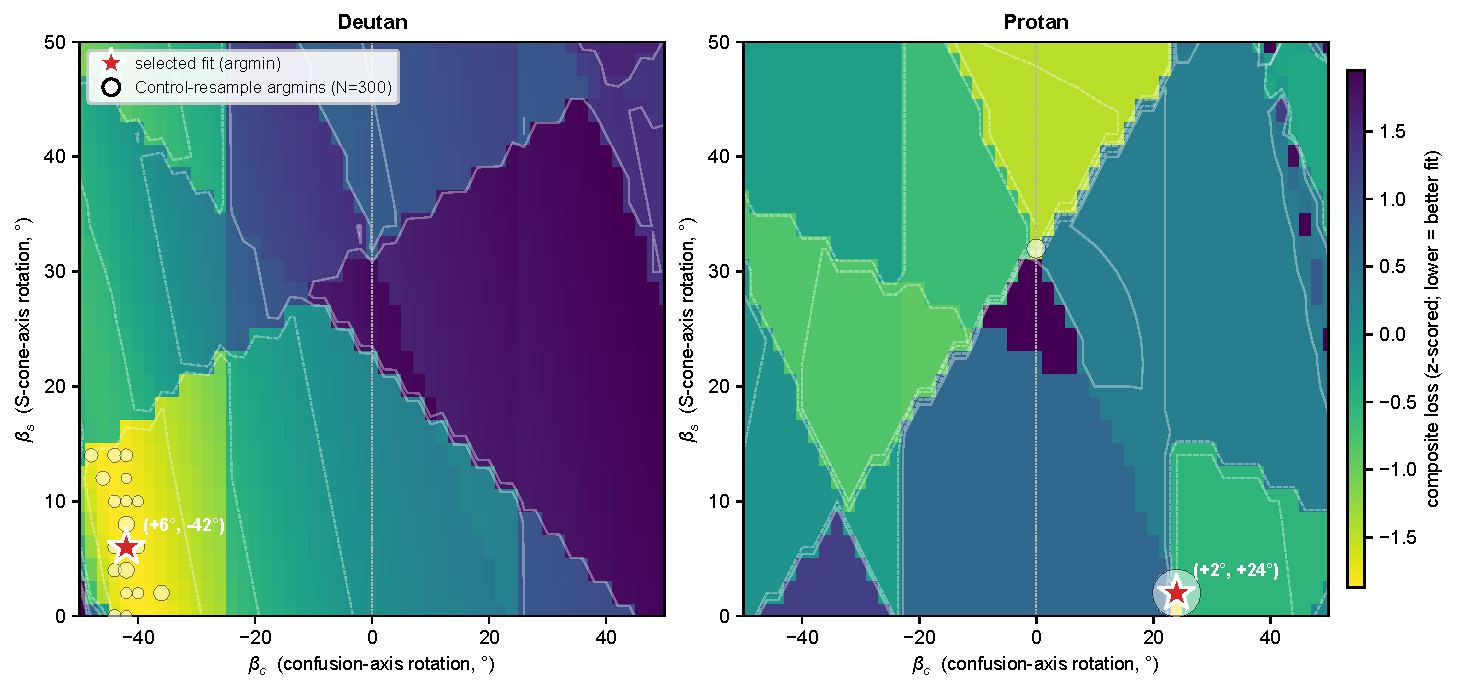
\includegraphics[width=\textwidth]{figS1_landscape}
  \caption{\textbf{Per-subject loss landscape and parameter uncertainty.}
  The $z$-scored composite loss over the $(\beta_s, \beta_c)$ grid, reconstructed on the full seven-control pool, with lower values in yellow.
  The loss combination is $\gamma_{\rm OY} + L_{\rm RDM}^{(V2)}$ for the deutan participant and $\gamma_{\rm all} + L_{\rm RDM}^{(V1)}$ for the protan participant.
  The red star marks the argmin of that surface, at $(\hat\beta_s, \hat\beta_c) = (6^\circ, -42^\circ)$ for the deutan participant and $(2^\circ, +24^\circ)$ for the protan participant.
  It is a descriptive low-dimensional embedding of the distortion rather than a physiological point estimate.
  White points give the per-resample argmins over $N = 300$ control 5-train/2-test resamples.}
  \label{fig:landscape}
\end{figure}


% --------------------------------------------------------------------------
% ==== S13  Stability of the selected fits ====
% --------------------------------------------------------------------------

\suppsection{Stability of the selected fits}{app:fit_stability}

\paragraph{Control leave-one-out magnitude anchor.}
Both CVD estimates fall inside the corresponding control range, so parameter magnitude alone is a descriptive anchor rather than a test of CVD-versus-control specificity. Each of the $n = 7$ control participants was refit as a pseudo-CVD case with the remaining control pool as reference, under that participant's own selected loss. The deutan combination is $\gamma_{\rm OY} + L_{\rm RDM}^{(V2)}$ and the protan combination $\gamma_{\rm all} + L_{\rm RDM}^{(V1)}$. The deutan estimate is $\|\hat\beta\| = 42.4^\circ$ against a control range of $30.5^\circ$ to $58.1^\circ$ (mean $49.1^\circ$). The protan estimate is $24.1^\circ$ against $23.4^\circ$ to $55.5^\circ$ (mean $35.7^\circ$), close to the lower bound.

\paragraph{Sign stability across the two preprocessing pipelines.}
Each participant's selected loss combination was refit on the head-motion-corrected pipeline (\cref{app:uncorrected}) with every other element of the procedure held fixed, and the two participants diverge. The sign of $\hat\beta_c$ held for the deutan participant, whose median moved from $-42^\circ$ to $-46^\circ$ with the fraction of negative resamples at $1.000$ and $0.947$. It reversed for the protan participant, whose median moved from $+24^\circ$ to $-12^\circ$, with the head-motion-corrected pipeline returning $79.3\%$ negative resamples against none under the primary pipeline. The deutan fit was also more poorly conditioned on the second pipeline, the combined fraction of resamples reaching a grid boundary rising from $0.09$ to $0.72$, and those boundary solutions lie on the same side as the median, so they bear on the magnitude rather than on the sign. The psychophysical atoms are independent of preprocessing, so the neural atom is the sole component that differs between the two fits. We therefore report the deployed protan parameter as a frozen value and give it no physiological interpretation.

\paragraph{Resample structure.}
Each participant's selected fit is the global minimum of its loss surface on the full data (\cref{fig:landscape}), and the $(32^\circ, 0^\circ)$ solution lies in the secondary basin of the protan PCA landscape, so the two reductions disagree about which basin is the minimum. Across the 300 resamples $\hat\beta_c$ concentrates at $-42^\circ$ and $-44^\circ$ ($202$ of $300$) and stays within $[-48^\circ, -36^\circ]$, whereas $\hat\beta_s$ is distributed almost uniformly from $0^\circ$ to $14^\circ$.

\paragraph{Gate statistics and neural-term ablation.}
Table~\ref{tab:fit_stability} collects the statistics that describe how each selected cell was reached and how stable it is. The separation block reports the precondition that admitted a $\Delta$RDM atom at a given ROI (\S\ref{sec:methods:selection}). The ablation block refits each participant's selected combination with the psychophysical atoms alone and with the $\Delta$RDM atom alone, holding every other element of the procedure fixed, so the three argmins are directly comparable. All entries are medians over the same $N = 300$ control 5-train/2-test resamples, on the PCA-basis loss unless the row names the SRM basis.

\begin{table}[htbp]
  \caption{Gate statistics, neural-term ablation, and resample stability for the two selected fits. Separation $d$ is the standardized distance between the participant and the control distribution at each ROI, and the $\Delta$RDM atom was admissible only where it was positive and exceeded the pre-set threshold (\S\ref{sec:methods:selection}), which left all four ROIs in the deutan participant and V1 alone in the protan participant. $\Delta\overline{L}$ is the change in an atom's held-out loss at the selected cell relative to the no-distortion cell $(0^\circ, 0^\circ)$, with negative values favoring the fitted distortion, and the fold count gives how many of the seven leave-one-out folds favor it. The boundary-saturation rate is the fraction of resamples whose solution reached a grid edge. Parameter IQRs are given as $(\beta_s, \beta_c)$.}
  \label{tab:fit_stability}
  \centering
  \small
  \begin{tabular}{lcc}
    \toprule
    & Deutan & Protan \\ \midrule
    \multicolumn{3}{l}{\emph{Separation precondition}} \\
    \quad $d$ at V1 / V2 / V3 / hV4 & $2.31$ / $1.94$ / $0.86$ / $2.19$ & $0.81$ / $-0.23$ / $-0.48$ / $-0.24$ \\
    \quad Loss combinations passing the gate & 25 & 4 \\ \midrule
    \multicolumn{3}{l}{\emph{Held-out generalization of the selected cell}} \\
    \quad Grid percentile & $4.6\%$ & $8.1\%$ \\
    \quad $\Delta\overline{L}$, psychophysical atom & $-13.85$ (5 of 7) & $+0.01$ (3 of 7) \\
    \quad $\Delta\overline{L}$, $\Delta$RDM atom & $-0.41$ (7 of 7) & $-0.47$ (7 of 7) \\ \midrule
    \multicolumn{3}{l}{\emph{Neural-term ablation (argmin)}} \\
    \quad Psychophysical atoms alone & $(16^\circ, -44^\circ)$ & $(26^\circ, +4^\circ)$ \\
    \quad $\Delta$RDM atom alone & $(4^\circ, -26^\circ)$ & $(0^\circ, +24^\circ)$ \\
    \quad Selected combination & $(6^\circ, -42^\circ)$ & $(2^\circ, +24^\circ)$ \\
    \quad Selected combination, SRM basis & $(8^\circ, -42^\circ)$ & $(32^\circ, 0^\circ)$ \\ \midrule
    \multicolumn{3}{l}{\emph{Resample stability, psychophysical alone $\rightarrow$ selected}} \\
    \quad Boundary-saturation rate & $0.23 \rightarrow 0.09$ & $0.00 \rightarrow 0.00$ \\
    \quad Parameter IQR, PCA basis & $(18^\circ, 6^\circ) \rightarrow (8^\circ, 2^\circ)$ & $(6^\circ, 4^\circ) \rightarrow (0^\circ, 0^\circ)$ \\
    \quad Parameter IQR, SRM basis & $(18^\circ, 6^\circ) \rightarrow (10^\circ, 4^\circ)$ & $(6^\circ, 4^\circ) \rightarrow (0^\circ, 2^\circ)$ \\
    \bottomrule
  \end{tabular}
\end{table}


\suppsection{Filter-evaluation session design and comparator}{app:filter_eval}

\paragraph{Comparator.}
The deployed comparator was the macOS accessibility Color Filter (System Settings $>$ Accessibility $>$ Display, build 26.5.1), set at an intensity the participant self-tuned before scanning. It is the unmodified shipping product, an operating-system-level post-display transform. We compared against it rather than a re-implemented retinal-simulation transform so that the comparator is the correction an end user actually encounters. The individualized filter was rendered directly in PsychoPy from the frozen per-subject pre-image.

\paragraph{Acquisition.}
Eight fMRI runs were acquired in ABBA-counterbalanced order, four per filter. Scanner time set this count, since six runs per condition would run roughly 90 minutes, beyond the 60--75-minute window over which participant attention and head motion stay acceptable. Four runs per condition take about 60 minutes, at the lower edge of that window.

\paragraph{Run-count adequacy.}
Four runs preserve the Session-1 separation between the control mean and the two CVD cases at hV4. Across all $\binom{6}{n}$ subsets of the six-run Session-1 data, hV4 LOCO adjacent accuracy held that separation at every run count down to four (\cref{fig:adjacc_saturation}). At $n = 4$ the control mean reached $0.45$ against $0.46$ at six runs and stayed above the $0.25$ chance level, while both CVD participants stayed below it (deutan $0.23$, protan $0.14$, single-case $d_{cc} < -2$ in both). Four runs nonetheless fall below the count recommended for fine-grained RDM-based model comparison, so the second session targets movement toward or away from the control reference rather than adjudication between model classes.

The filter conditions each have four runs, whereas the Session-1 control reference and the unfiltered baseline each have six. Noise in either pattern inflates disparity and RDM similarity, so an unmatched comparison would penalize the filter conditions twice, once against the baseline and once against the control distribution that the single-case test uses. Every neural index is therefore reported run-matched. For the interpolation indices the control reference is subsampled to four runs. For the geometry indices both the control means and the unfiltered baseline are rebuilt from four runs, exhaustively over all $\binom{6}{4} = 15$ subsets, with the shared response model refitted within each subset and the resulting metrics averaged (\texttt{exp2\_runmatched\_geometry.py}). The filter conditions themselves are never subsampled. The control reference comprises $n = 7$ controls at V1--V3 and $n = 6$ at hV4, where one control has too few voxels. Matching raises the protan V1 RDM similarity of the unfiltered baseline from $0.25$ to $0.33$, which places the individualized filter's value below that baseline rather than above it, and leaves the ordering of conditions unchanged on all four indices.
% TERMINOLOGY (resolved 2026-08-05): was "RDM-based model discrimination"; changed to
% "model comparison". "discrimination" is now reserved paper-wide for the behavioral
% JND construct; the neural LORO construct is "color classification".

\begin{figure}[tb]
  \renewcommand{\thefigure}{S\arabic{figure}}  % see the note on the first supplementary figure
  \centering
  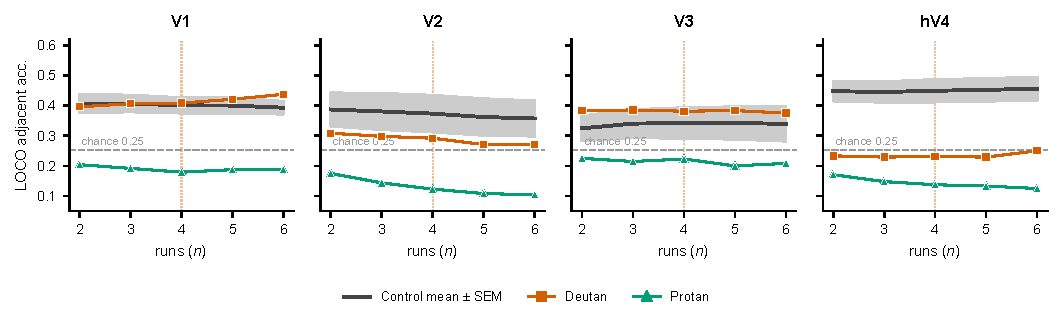
\includegraphics[width=\linewidth]{figS2_adjacc_saturation}
  \caption{\textbf{Hue-interpolation adjacent accuracy as a function of the number of runs.} LOCO adjacent accuracy (six-channel basis, OLS pseudoinverse decoder) as a function of the number of runs $n$, computed over all $\binom{6}{n}$ run subsets of the Session-1 data, per ROI. Black line, control mean $\pm$ SEM (shaded band); dashed line, the $0.25$ chance level; markers, the two CVD single cases (deutan, protan). The orange guide marks the deployed $n = 4$.}
  \label{fig:adjacc_saturation}
\end{figure}

\paragraph{Single-case inference.}
Each condition's neural index was compared to the control distribution as the case-control effect size $d_{cc}$ (\S\ref{sec:methods:stats}), reported in place of an inferential $p$ because the grand-mean permutation null is biased for this design. Robustness was assessed by leave-one-run separation, the contrast holding after any single run is dropped, and by re-extracting both conditions on the no-filter baseline voxel set.

% --------------------------------------------------------------------------
% ==== S15  Second-session outcomes by condition ====
% Split from the former "Filter-evaluation session design and comparator"
% on 2026-09-04: the design half and the condition-level results half each
% carry their own exhibits (words_trimming.md §5.4).
% --------------------------------------------------------------------------

\suppsection{Second-session outcomes by condition}{app:exp2_outcomes}

Each index below is reported for the unfiltered Session-1 baseline (NF), the deployed accessibility filter (Dep), and the individualized filter (Ind), run-matched as described in \cref{app:filter_eval}.

\paragraph{Hue identification (8AFC).}
Identification accuracy stayed at or above the Session-1 baseline under the individualized filter in both participants (\cref{tab:exp2_8afc}). This task entered neither fitting term, so it is a prospective test of the filters (\S\ref{sec:results:filter_eval}).

\begin{table}[tb]
  \centering
  \caption{\textbf{Second-session hue identification (8AFC).} Accuracy over $n = 64$ trials per cell with the 95\% Wilson score interval. Chance $= 0.125$. NF, no-filter (Session-1 baseline); Dep, deployed accessibility filter; Ind, individualized filter.}
  \label{tab:exp2_8afc}
  \begin{tabular}{llcc}
    \toprule
    Participant & Condition & Accuracy & 95\% CI \\
    \midrule
    Deutan & NF  & 0.81 & $[0.70, 0.89]$ \\
                    & Dep & 0.97 & $[0.89, 0.99]$ \\
                    & Ind & 0.97 & $[0.89, 0.99]$ \\
    \midrule
    Protan & NF  & 1.00 & $[0.94, 1.00]$ \\
                    & Dep & 0.86 & $[0.75, 0.92]$ \\
                    & Ind & 0.98 & $[0.92, 1.00]$ \\
    \bottomrule
  \end{tabular}
\end{table}

\paragraph{Hue classification (LORO).}
The displayed hues remained decodable under both filters (\cref{tab:exp2_loro}). Every cell stayed above the $0.125$ chance level. The lowest cell, $0.50$ at hV4 under the individualized filter in the deutan participant, lies below the control range of $0.71$ to $0.77$.

\begin{table}[tb]
  \centering
  \caption{\textbf{Second-session hue classification (LORO eight-way classification accuracy).} Chance $= 0.125$. NF, no-filter (Session-1 baseline); Dep, deployed accessibility filter; Ind, individualized filter. Controls, mean ($n = 7$).}
  \label{tab:exp2_loro}
  \begin{tabular}{lccccccc}
    \toprule
     & & \multicolumn{3}{c}{Deutan} & \multicolumn{3}{c}{Protan} \\
    \cmidrule(lr){3-5} \cmidrule(lr){6-8}
    ROI & Controls & NF & Dep & Ind & NF & Dep & Ind \\
    \midrule
    V1  & 0.71 & 0.79 & 0.84 & 0.72 & 0.79 & 0.91 & 0.66 \\
    V2  & 0.71 & 0.79 & 0.69 & 0.62 & 0.83 & 0.75 & 0.72 \\
    V3  & 0.77 & 0.67 & 0.78 & 0.69 & 0.81 & 1.00 & 0.69 \\
    hV4 & 0.75 & 0.73 & 0.88 & 0.50 & 0.71 & 0.84 & 0.69 \\
    \bottomrule
  \end{tabular}
\end{table}

\paragraph{Interpolation and geometry by condition.}
The three neural indices of the second session appear in \cref{tab:exp2_geometry} at each participant's target region, with the control reference and the single-case effect size for every condition.

\begin{table}[tb]
  \centering
  \caption{\textbf{Second-session interpolation and representational geometry.} All entries are run-matched (four runs per cell). NF, no-filter (Session-1 baseline); Dep, deployed accessibility filter; Ind, individualized filter. Parenthetical values are Crawford--Howell single-case effect sizes $d_{cc}$ against the control distribution. For adjacent accuracy the control entry is the mean $\pm$ SD over $n = 6$ controls at hV4 and the analytic chance level is $0.25$. For SRM disparity the control entry is the mean over $n = 7$ controls and lower values are more control-like. For RDM similarity the control entry is the leave-one-out self-consistency, a single value with no dispersion, so no effect size is defined and higher values are more control-like. The target region is the one at which each participant's Session-1 disparity was elevated, V2 for the deutan and V1 for the protan participant.}
  \label{tab:exp2_geometry}
  \small
  \begin{tabular}{lcccc}
    \toprule
    Index & Controls & NF & Dep & Ind \\
    \midrule
    \multicolumn{5}{l}{\emph{Deutan}} \\
    \quad hV4 adjacent accuracy & $0.46 \pm 0.11$ & $0.23$ ($-2.11$) & $0.25$ ($-1.94$) & $0.31$ ($-1.35$) \\
    \quad V2 SRM disparity & $0.44$ & $0.68$ ($2.69$) & $0.87$ ($4.93$) & $0.77$ ($3.73$) \\
    \quad V2 RDM similarity & $0.59$ & $0.42$ & $0.16$ & $0.05$ \\
    \midrule
    \multicolumn{5}{l}{\emph{Protan}} \\
    \quad hV4 adjacent accuracy & $0.46 \pm 0.11$ & $0.14$ ($-2.99$) & $0.19$ ($-2.52$) & $0.06$ ($-3.70$) \\
    \quad V1 SRM disparity & $0.43$ & $0.70$ ($3.92$) & $0.66$ ($3.29$) & $0.63$ ($2.84$) \\
    \quad V1 RDM similarity & $0.66$ & $0.33$ & $0.38$ & $0.26$ \\
    \bottomrule
  \end{tabular}
\end{table}

\paragraph{Forward-tuning encoding index.}
The forward-tuning correlation $\rho$ is the Pearson correlation between the predicted and the observed voxel pattern, averaged over the eight held-out hues. It indexes the encoding fit rather than the decoding accuracy on which the comparison rests. Figure~\ref{fig:forward_tuning} shows this index against the reference hue map, reported as corroboration only, since it lies outside the validated Session-1 decoding pipeline. In the deutan participant the individualized filter approaches the control level at hV4 ($\rho = +0.18$ against controls $+0.21$) while under the deployed filter it falls to $\rho = -0.39$. In the protan participant the three conditions do not separate, all reaching $\rho \approx -0.02$ at hV4.

\begin{figure}[tb]
  \renewcommand{\thefigure}{S\arabic{figure}}  % see note on the previous figure
  \centering
  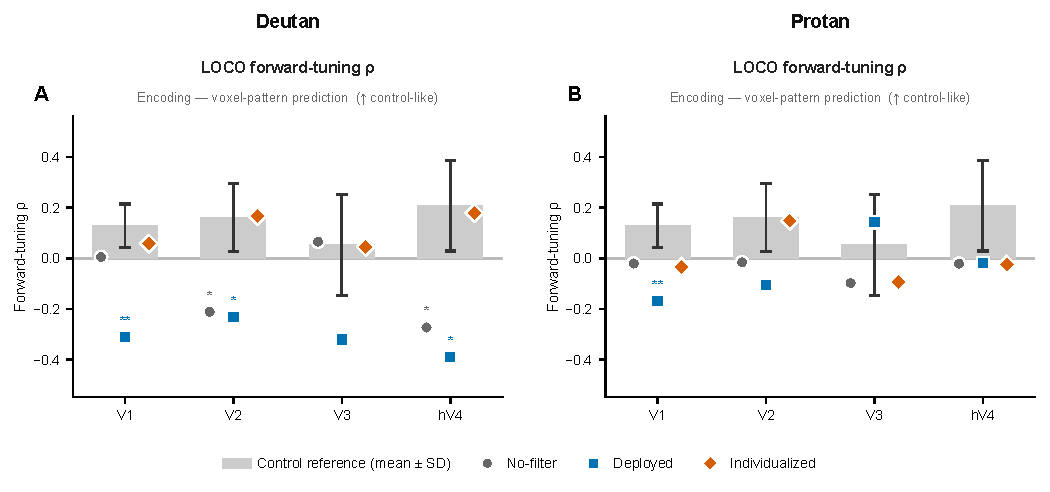
\includegraphics[width=\linewidth]{figS3_forward_tuning}
  \caption{\textbf{Forward-tuning encoding index (corroboration only).} LOCO forward-tuning correlation $\rho$ to the reference hue map across V1--hV4, for the deutan (left) and protan (right) participants ($\uparrow$ control-like). Gray bars, control reference (mean $\pm$ SD, $n = 7$); markers, no-filter (gray circle), deployed accessibility filter (blue square), individualized filter (orange diamond). Stars, Crawford--Howell single-case deviation from the control distribution ($^{*}p<.05$, $^{**}p<.01$).}
  \label{fig:forward_tuning}
\end{figure}


% ========== Section 14: Effect Sizes ==========

% --------------------------------------------------------------------------
% ==== S16  Statistical analysis and effect sizes ====
% Merger of the former "Effect sizes for single-case comparisons" and
% "Statistical analysis" sections (2026-09-04). The two defined d_cc in terms
% of each other; Methods §sec:methods:stats now points here once.
% The cross-subject encoder-transfer comparison moved to \cref{app:decoders},
% where it belongs with the decoder results (words_trimming.md §5.4).
% --------------------------------------------------------------------------

\suppsection{Statistical analysis and effect sizes}{app:statistics}

Unless noted otherwise, the significance threshold was $\alpha = 0.05$. False Discovery Rate correction \parencite{benjamini1995} was applied within two pre-specified families alone, the RDM hue-pair comparisons ($q = 0.05$, 28 pairs per participant) and the six parameter-identifiability checks (\cref{sec:methods:identifiability}). The exploratory per-hue vulnerability comparisons and the per-pair identification tests, including the blue-hue deficit, are reported one-tailed and uncorrected. Individual CVD participants were compared to the control distribution using the \textcite{crawford1998} modified $t$-test,

with the tail set by the pre-specified direction of each endpoint, one-tailed upper for disparity, one-tailed lower for interpolation, and two-tailed for classification and for the activation metrics.

Single-case effect sizes are the case-control index $d_{cc} = (x_{\rm case} - \bar{x}_{\rm ctrl}) / s_{\rm ctrl} = t\sqrt{(n+1)/n}$, where $n$ is the control sample size used in the test. Mann--Whitney $U$ tests use the rank-biserial correlation $r_{\rm rb}$ as their effect size, and group-level effect sizes are Hedges' $g$ \parencite{hedges1985}. Effect sizes for the single-case interpolation comparisons appear in \cref{tab:effect_sizes}, and the geometric-disparity effect sizes appear beside their $t$ statistics in \cref{tab:disparity_loso}. Single-case comparisons of within-subject LORO accuracy against the control distribution reached $|d_{cc}|$ between $0.25$ and $1.58$ across the eight participant-by-ROI tests, with all $p \geq 0.189$ (two-tailed). The largest deviation was the deutan participant at V3 ($d_{cc} = -1.58$), and at hV4 both participants gave $d_{cc} = -1.08$ ($p = 0.352$).

\begin{table}[h]
\centering
\caption{Effect sizes for the single-case hue-interpolation comparisons at hV4 (main text, \S\ref{sec:results:loco}). Crawford--Howell case-control effect size $d_{cc} = t\sqrt{(n+1)/n}$ against the $n = 7$ control distribution, one-tailed. Per-hue tests are uncorrected and exploratory across eight hues. Both CVD participants share identical statistics at the three hues where adjacent accuracy is zero. Blue lies just above the conventional threshold and is the largest per-hue deviation.}
\label{tab:effect_sizes}
\begin{tabular}{lccc}
\toprule
Comparison (hV4) & $t$ & $p$ & $d_{cc}$ \\
\midrule
LOCO adjacent accuracy, deutan & $-1.89$ & $0.054$ & $-2.02$ \\
LOCO adjacent accuracy, protan & $-3.04$ & $0.012$ & $-3.25$ \\
\midrule
\multicolumn{4}{l}{\emph{Per-hue adjacent accuracy (one-tailed, exploratory; both participants)}} \\
Blue & $-1.93$ & $0.051$ & $-2.06$ \\
Purple & $-0.79$ & $0.229$ & $-0.85$ \\
Magenta & $-1.47$ & $0.096$ & $-1.57$ \\
\bottomrule
\end{tabular}
\end{table}


\suppsection{Alignment robustness of the within-subject readouts}{app:alignment}

The two alignment spaces agree on the pattern on which the Results rest. LORO and LOCO are trained and tested within a single participant, so the main text computes them on the Procrustes-aligned amplitudes, which retain that participant's voxels at full resolution, and SRM enters only where a comparison spans participants. \cref{tab:alignment} gives both readouts in the Procrustes space, and the hue-channel-basis rows of \cref{tab:loro_decoders,tab:loco_decoders} give the same readouts in the SRM space.

Classification stays above the $0.125$ chance level for both CVD participants at every region in both spaces, with the lowest cell at $0.312$. Interpolation at hV4 remains reduced in both participants in both spaces, and the ordering of the two participants is preserved. Procrustes alignment yields the higher control-mean accuracy at all four regions for classification and at three of the four for interpolation, and it is the higher of the two spaces in 26 of the 36 participant-by-region classification cells. This follows from the dimensionality reduction in SRM discarding response variance that a within-subject readout can otherwise use.

The spaces differ at V1 classification, where SRM places both CVD participants above the control mean ($d_{cc} = +0.59$ and $+0.79$) while Procrustes places them slightly below ($d_{cc} = -0.25$ for both). Every single-case classification comparison stayed short of significance in both spaces.

\begin{table}[h]
\centering
\caption{Hue-channel basis readouts in the Procrustes-aligned space, which the main text reports. LORO is eight-way classification accuracy (chance $0.125$); LOCO is adjacent accuracy (analytic chance $0.25$). The control column is the mean over $n = 7$. The SRM-aligned counterpart of every cell appears in the forward-encoding rows of \cref{tab:loro_decoders,tab:loco_decoders}.}
\label{tab:alignment}
\begin{tabular}{lcccccc}
\toprule
& \multicolumn{3}{c}{LORO classification} & \multicolumn{3}{c}{LOCO interpolation} \\
\cmidrule(lr){2-4}\cmidrule(lr){5-7}
Region & Controls & deutan & protan & Controls & deutan & protan \\
\midrule
V1  & $0.580$ & $0.562$ & $0.562$ & $0.393$ & $0.437$ & $0.188$ \\
V2  & $0.607$ & $0.521$ & $0.562$ & $0.357$ & $0.271$ & $0.104$ \\
V3  & $0.574$ & $0.396$ & $0.458$ & $0.339$ & $0.375$ & $0.208$ \\
hV4 & $0.488$ & $0.375$ & $0.375$ & $0.456$ & $0.250$ & $0.125$ \\
\bottomrule
\end{tabular}
\end{table}


% --------------------------------------------------------------------------
% ==== S17  (was Supplementary/S18_geometry_validity.tex) ====
% --------------------------------------------------------------------------
% Supplementary S16 — Validity of the geometric comparison
% 2026-08-07
% Governing document: docs/PAPER/REVISION_PLAN_MOTION_GEOMETRY_2026-08-06.md §S18 (rule R5).
% Source numbers: analysis/phase2_SRM_across_between/results/RESULTS_GEOMETRY_VALIDITY_2026-08-05.md
%   §1 (control positive control), §2 (color specificity), §4 (cyclic shift)
% Raw outputs: analysis/future_phase1_sensitivity/results/{with_residuals,hmc_v2}/color_correspondence/frozen_permutation.json,
%   analysis/validation/results/cyclic_shift_disparity.json (hmc_v2 variant not yet computed)
% Counts and BH-FDR recomputed from the JSON on 2026-08-07:
%   35 cells, 16 raw p<.05 (the "15" in RESULTS_GEOMETRY_VALIDITY §2 prose is a
%   miscount of its own table), 7 surviving BH; motion-regressed 18 raw / 15 BH.
% The cyclic-shift gain is referred to the control gain distribution, which is computed
%   under the same minimum-over-eight rule and therefore absorbs the same selection
%   bias. hV4 shift gains are omitted: the ROI carries no geometric endpoint, and
%   the motion-regressed control gain SD there collapses to 0.38%.

\suppsection{Validity of the geometric comparison}{app:geometry_validity}

The color-correspondence permutation has power only when the shared projection is held fixed, since re-estimating it at each permutation allows the re-fit to absorb the permutation. The permutation asks whether a participant's colors map onto the control geometry in the identity order, which differs from the color-label permutation null of the main text, where the question is whether the control group interpolates above chance in a region. We tested both variants on the controls, in whom color structure is established. Re-estimation detected 0 of 7 at V1, V2 and V3 and 0 of 6 at hV4, with mean permutation $z$ near zero in every ROI, whereas freezing the projection recovered detection, reaching 5 of 7 at V3 and 2 to 3 of 7 elsewhere (\cref{tab:frozen_control}). Every color-specificity result below uses the frozen projection.

\begin{table}[h]
\centering
\caption{Color-correspondence permutation on the controls, used as a positive control. Detection counts and mean permutation $z$ under a projection re-estimated at each permutation and under a frozen projection. Lower $z$ indicates a better identity correspondence than the shuffled null.}
\label{tab:frozen_control}
\begin{tabular}{lccccc}
\toprule
 & & \multicolumn{2}{c}{Re-estimated} & \multicolumn{2}{c}{Frozen} \\
\cmidrule(lr){3-4}\cmidrule(lr){5-6}
ROI & $n$ & detected & mean $z$ & detected & mean $z$ \\
\midrule
V1  & 7 & 0 & $-0.04$ & 2 & $-1.58$ \\
V2  & 7 & 0 & $-0.04$ & 3 & $-1.00$ \\
V3  & 7 & 0 & $-0.78$ & 5 & $-2.39$ \\
hV4 & 6 & 0 & $+0.06$ & 2 & $-1.07$ \\
\bottomrule
\end{tabular}
\end{table}

Both CVD participants showed color-specific geometry. The deutan participant reached $p = .002$ at V2, the lowest V2 value among the nine participants, and $p = .024$ at V3. The protan participant reached $p = .001$ at V3 and $p = .013$ at V2, while V1 returned $p = .758$. Across the 35 participant-by-ROI cells, 16 fell below $.05$ against a chance expectation of $1.8$, and 7 survived Benjamini--Hochberg correction over all 35 (\cref{tab:color_specificity}). Two of the survivors belong to the CVD participants, the deutan V2 cell ($q = .018$) and the protan V3 cell ($q = .012$). V3 showed color specificity most broadly, with 5 of its 9 cells surviving.

\begin{table}[h]
\centering
\caption{Color-correspondence permutation under the frozen projection, one cell per participant and region, in the two preprocessing pipelines. Entries give $p_{\rm perm}$ against $N = 1{,}000$ permutations. Seven cells survive Benjamini--Hochberg correction across the 35 cells of the primary pipeline and none survive it in the head-motion-corrected pipeline.}
\label{tab:color_specificity}
\begin{tabular}{lcccccccc}
\toprule
 & \multicolumn{4}{c}{Primary} & \multicolumn{4}{c}{Head-motion correction} \\
\cmidrule(lr){2-5}\cmidrule(lr){6-9}
Participant & V1 & V2 & V3 & hV4 & V1 & V2 & V3 & hV4 \\
\midrule
Control 1 & $0.088$ & $0.020$ & $0.062$ & $0.393$ & $0.012$ & $0.072$ & $0.018$ & $0.290$ \\
Control 2 & $0.001$ & $0.016$ & $0.004$ & $0.136$ & $0.437$ & $0.420$ & $0.191$ & $0.019$ \\
Control 3 & $0.109$ & $0.520$ & $0.255$ & $0.272$ & $0.325$ & $0.113$ & $0.176$ & $0.101$ \\
Control 4 & $0.152$ & $0.014$ & $0.001$ & $0.041$ & $0.420$ & $0.006$ & $0.015$ & $0.173$ \\
Control 5 & $0.057$ & $0.773$ & $0.034$ & $0.031$ & $0.079$ & $0.194$ & $0.032$ & $0.038$ \\
Control 6 & $0.407$ & $0.290$ & $0.009$ & $0.220$ & $0.373$ & $0.117$ & $0.010$ & $0.012$ \\
Control 7 & $0.034$ & $0.159$ & $0.004$ & --- & $0.008$ & $0.005$ & $0.391$ & --- \\
\textbf{Deutan} & $0.105$ & $0.002$ & $0.024$ & $0.273$ & $0.022$ & $0.003$ & $0.047$ & $0.257$ \\
\textbf{Protan} & $0.758$ & $0.013$ & $0.001$ & $0.129$ & $0.010$ & $0.148$ & $0.053$ & $0.815$ \\
\bottomrule
\end{tabular}
\end{table}

Under head-motion correction 15 cells fell below $.05$ and none survived correction. The deutan V2 cell remained at its nominal value across the two pipelines ($p = .002$ and $p = .003$) while its corrected value moved from $q = .018$ to $q = .053$, and the protan V1 cell moved from $p = .758$ to $p = .010$. Individual cells of this grid are descriptive and support no claim in the main text.

The protan participant's V1 correspondence is displaced by one hue step, and the failure is not one of signal. That participant's V1 split-half pattern reliability reaches $.847$, above the highest control value, and eight-way classification there reaches $0.79$ against a chance level of $0.125$. Rotating the color labels by $45^\circ$ lowered Procrustes disparity from $1.037$ to $0.788$, a gain of $24.0\%$. We referred that gain to the distribution of shift gains across the seven controls ($3.5 \pm 5.9\%$), which is computed under the same minimum-over-eight rule and is therefore subject to the same selection bias. The protan gain exceeded that distribution (Crawford--Howell $t = 3.22$, $p = .009$, $d_{cc} = 3.44$), and the rotated geometry sat below the control mean disparity of $0.839 \pm 0.087$. The same rotation raised the second-order RSA similarity from $\rho \approx 0.00$ to $\rho = +0.52$, against a control mean of $0.45$, exceeding its own selection-bias null ($z = +5.02$, $p = .002$, $p_{\rm adj} = .032$). Disparity at this region is nonetheless elevated in both pipelines, so the departure is not accounted for by a rigid relabeling alone. The account applies to the primary pipeline, since that cell is no longer null under head-motion correction. The deutan participant showed the identity mapping as optimal at V1, V2 and V3.

Which rearrangement restores control-level similarity remains open. Under the SRM basis a $225^\circ$ shift ($+0.50$) is close to the $315^\circ$ optimum ($+0.52$). Under the PCA basis the optimum falls at $135^\circ$ ($p = .048$, which does not survive correction).
% Superseded sources: docs/PAPER/Supplementary/archive/ (gitignored)
% ============================================================================

\renewcommand{\thetable}{S\arabic{table}}\setcounter{table}{0}


% ========== Section 1: Session-1 hue-discrimination thresholds ==========

\suppsection{Session-1 hue-discrimination thresholds}{app:jnd_baseline}

Session-1 threshold elevations followed each participant's subtype (\cref{tab:jnd_baseline}). The threshold is the staircase level $t$, the fraction of the pair's full CIE $LCh$ separation at which the two discs were discriminated (\S\ref{sec:methods:psychophysical}), so smaller values indicate finer discrimination. The ratio $\gamma$ divides the participant's threshold by the control mean, and $z$ expresses the same difference in control standard deviations over the seven controls. Pairs are grouped by the axis each was chosen to probe, and that assignment was fixed before any threshold was collected.

Each pair was measured by two interleaved staircases from starting levels $t = 0.8$ and $t = 0.5$, both following a 1-up/1-down rule with a step of $0.15$ until the second reversal and $0.03$ thereafter. A staircase terminated at eight reversals and at least 20 trials, extended by two further reversals whenever the SD of the last six reversal levels exceeded $0.10$.

Elevation localized to the axis each participant's subtype predicts. The deutan participant exceeded $z = +4$ on both deutan-axis pairs and on the yellow--purple S-cone pair, and the protan participant exceeded the control range on the protan-axis pair green--blue alone. Both participants remained inside the control range on the $180^\circ$ control pair, which places the elevation on specific axes rather than on overall sensitivity. These thresholds enter the psychophysical loss atoms of \S\ref{sec:methods:candidates}, and the same eight pairs supply the pre-filter baseline of the filter evaluation (\S\ref{sec:results:filter_eval}).

\begin{table}[h]
\centering
\caption{Session-1 hue-discrimination thresholds without a filter. The control column is the mean $\pm$ SD over the seven controls. $\gamma$ is the ratio to the control mean and $z$ the deviation in control standard deviations. Bold: $|z| \geq 2$. Two staircases returned an incorrect response at the largest presentable separation, both of them the deutan participant's orange--yellow pair, so that threshold is a lower bound rather than an estimate. It is the only such pair among the 208 staircases collected in this study.}
\label{tab:jnd_baseline}
\setlength{\tabcolsep}{4pt}
\begin{tabular}{llcccccccc}
\toprule
& & \multicolumn{2}{c}{Controls ($n = 7$)} & \multicolumn{3}{c}{Deutan} & \multicolumn{3}{c}{Protan} \\
\cmidrule(lr){3-4}\cmidrule(lr){5-7}\cmidrule(lr){8-10}
Axis probed & Pair & mean & SD & $t$ & $\gamma$ & $z$ & $t$ & $\gamma$ & $z$ \\
\midrule
Deutan confusion & orange--yellow & $0.278$ & $0.135$ & $0.840$ & $\mathbf{3.02}$ & $\mathbf{+4.15}$ & $0.193$ & $0.69$ & $-0.63$ \\
                 & yellow--green  & $0.090$ & $0.044$ & $0.278$ & $\mathbf{3.10}$ & $\mathbf{+4.32}$ & $0.128$ & $1.42$ & $+0.87$ \\
\midrule
Protan confusion & green--blue    & $0.079$ & $0.032$ & $0.078$ & $0.98$ & $-0.06$ & $0.155$ & $\mathbf{1.95}$ & $\mathbf{+2.36}$ \\
                 & cyan--magenta  & $0.042$ & $0.017$ & $0.040$ & $0.95$ & $-0.13$ & $0.038$ & $0.89$ & $-0.28$ \\
\midrule
S-cone           & yellow--purple & $0.022$ & $0.006$ & $0.063$ & $\mathbf{2.87}$ & $\mathbf{+6.70}$ & $0.028$ & $1.26$ & $+0.94$ \\
                 & blue--purple   & $0.164$ & $0.093$ & $0.120$ & $0.73$ & $-0.48$ & $0.148$ & $0.90$ & $-0.18$ \\
                 & red--orange    & $0.124$ & $0.072$ & $0.063$ & $0.50$ & $-0.85$ & $0.075$ & $0.61$ & $-0.68$ \\
\midrule
Control          & red--cyan      & $0.034$ & $0.015$ & $0.015$ & $0.45$ & $-1.23$ & $0.015$ & $0.45$ & $-1.23$ \\
\midrule
\multicolumn{7}{l}{Mean $|z|$ over the eight pairs \quad Deutan $2.24$ \quad Protan $0.90$} & & & \\
\bottomrule
\end{tabular}
\end{table}


The deutan orange--yellow threshold is a lower bound. Both of its staircases remained at the top of the presented range throughout and returned incorrect responses at the largest separation the task presents. Censoring understates the baseline deficit and therefore the improvement recorded under either filter, so the value is reported unadjusted.

\begin{table}[h]\centering\small
\caption{Both staircase estimates for every hue pair, given as high-start/low-start in units of the rendered separation. Bold marks the cells whose two estimates differ by more than 0.10. Thresholds reported elsewhere are the mean of the two.}
\label{tab:staircase_pairs}
\begin{tabular}{lcccccc}
\toprule
 & \multicolumn{3}{c}{Deutan} & \multicolumn{3}{c}{Protan} \\
\cmidrule(lr){2-4}\cmidrule(lr){5-7}
Pair & Session 1 & Deployed & Individualized & Session 1 & Deployed & Individualized \\
\midrule
red--orange & 0.060/0.065 & 0.160/0.210 & 0.140/0.130 & 0.075/0.075 & 0.110/0.145 & 0.070/0.055 \\
orange--yellow & 0.870/0.810 & 0.080/0.110 & 0.060/0.032 & 0.175/0.210 & 0.170/0.185 & \textbf{0.715/0.200} \\
yellow--green & 0.280/0.275 & 0.090/0.075 & 0.145/0.165 & 0.125/0.130 & 0.057/0.050 & 0.055/0.065 \\
green--blue & 0.065/0.090 & 0.150/0.110 & 0.045/0.060 & 0.145/0.165 & 0.260/0.225 & 0.135/0.080 \\
blue--purple & 0.115/0.125 & 0.050/0.095 & 0.110/0.200 & 0.125/0.170 & 0.135/0.110 & 0.150/0.105 \\
yellow--purple & 0.060/0.065 & 0.015/0.020 & 0.035/0.025 & 0.020/0.035 & 0.020/0.015 & 0.015/0.015 \\
red--cyan & 0.015/0.015 & 0.040/0.018 & 0.015/0.045 & 0.015/0.015 & 0.030/0.040 & 0.020/0.025 \\
cyan--magenta & 0.035/0.045 & 0.030/0.025 & 0.040/0.033 & 0.040/0.035 & 0.150/0.140 & 0.015/0.020 \\
\bottomrule\end{tabular}\end{table}

The two staircases of a pair agreed closely (\cref{tab:staircase_pairs}). They differed by a median of $0.015$ across the $104$ pairs, and three cells exceeded $0.10$. The largest, at $0.515$, is the protan participant's orange--yellow pair under the individualized filter, where one track settled at $0.715$ after answering correctly at a four-fold smaller separation earlier in the same block while its partner converged at $0.200$ on the same rendered stimuli. We attribute that cell to a single lapse and report every threshold as the unadjusted mean of the two tracks. Restricting it to the converged track would move the cell from $z = +1.33$ to $z = -0.58$ and the participant's mean $|z|$ from $0.93$ to $0.84$.



% --------------------------------------------------------------------------
% ==== Sections carrying a "% ========== Section N ==========" banner below
%      (was Methods/supplementary_content.tex, archived) ====
% --------------------------------------------------------------------------
% Supplementary Methods - Content Only
% To be included via \input{Methods/supplementary_content}


% --------------------------------------------------------------------------
% ==== S2  (was Supplementary/S17_uncorrected_artifacts.tex) ====
% --------------------------------------------------------------------------
% Supplementary S1 — Preprocessing pipelines and sensitivity analyses
% 2026-08-07
% Scope: slice timing, head motion, susceptibility distortion were all left
%   uncorrected in the analyzed pipeline. Motion has a sensitivity analysis;
%   distortion and coregistration are argued on structural grounds.
% Source numbers: analysis/phase2_SRM_across_between/results/RESULTS_MOTION_ARMS_2026-08-05.md
%   Coregistration stability: docs/PAPER/METHODS_REVISION_STATUS_2026-08-07.md §3

\suppsection{Preprocessing pipelines and sensitivity analyses}{app:uncorrected}

\paragraph{The two pipelines.}
Every neural endpoint of the first session was computed under two pipelines. The primary pipeline resampled each functional volume once by a transform identical for every volume in a run. The second composed each volume's MCFLIRT rigid-body realignment matrix with that transform before the same single resampling, so the two differ in the alignment method and share the number of resamplings. Head-motion correction lowered ROI temporal signal-to-noise ratio by $1.7$ to $2.7\%$. In both, the per-run linear and constant drift terms of the general linear model constituted the entire nuisance model, and both pipelines left slice timing, susceptibility distortion, and temporal filtering out. Within-run motion was estimated by registering every volume to its run's middle volume and summarized as framewise displacement \parencite{power2012}, with rotations converted to displacement on a 50\,mm sphere. Across the nine analyzed participants mean framewise displacement reached $0.318 \pm 0.044$\,mm (controls $0.313 \pm 0.042$, CVD $0.338 \pm 0.046$), and $16.2\%$ of volumes exceeded $0.5$\,mm.

\paragraph{Disparity under the two pipelines.}
The regional attribution of disparity depends on the pipeline (\cref{tab:motion_arms}). Procrustes disparity was recomputed under head-motion correction with every other element held fixed. The protan V1 elevation remained the largest deviation in that participant under both pipelines and weakened from $p = .007$ to $p = .077$. In the deutan participant the largest deviation moved from V2 to V1 and the V2 value reversed in sign. Under the leave-one-subject-out estimator the protan V1 cell of the primary pipeline reached significance alone.

\begin{table}[h]
\centering
\caption{Procrustes disparity by participant and region under head-motion correction. Entries give the Crawford--Howell one-tailed $t$ with $p$ in parentheses, against the control leave-one-out distribution ($n = 7$), for the common-space estimator and for the leave-one-subject-out estimator on which the inference rests. The primary pipeline appears in \cref{tab:disparity_loso}, which adds the case-control effect sizes. Individual cells of this grid are descriptive and support no claim in the main text.}
\label{tab:motion_arms}
\small
\begin{tabular}{llcc}
\toprule
Participant & Region & Crawford--Howell & Leave-one-subject-out \\
\midrule
Deutan & V1  & $2.4$ ($.027$) & $1.6$ ($.080$) \\
Deutan & V2  & $-1.0$ ($.825$) & $-0.6$ ($.723$) \\
Deutan & V3  & $0.6$ ($.293$) & $0.4$ ($.338$) \\
Deutan & hV4 & $0.4$ ($.351$) & $0.4$ ($.356$) \\
Protan & V1  & $1.6$ ($.077$) & $1.3$ ($.121$) \\
Protan & V2  & $1.0$ ($.186$) & $0.1$ ($.480$) \\
Protan & V3  & $1.1$ ($.151$) & $1.0$ ($.178$) \\
Protan & hV4 & $1.4$ ($.101$) & $1.1$ ($.159$) \\
\bottomrule
\end{tabular}
\end{table}

\paragraph{Classification and interpolation under the two pipelines.}
The two readouts dissociate under both pipelines (\cref{tab:interp_arms}). The control-group interpolation gate, the two single-case comparisons at hV4 (\S\ref{sec:results:loco}), and the eight-way classification readout (\S\ref{sec:results:loro}) were recomputed the same way. hV4 alone passes the control gate in both pipelines, and both participants remain below the control mean in both. Classification survives in both. The lowest CVD cell across the four regions reaches $0.375$ under the primary pipeline and $0.229$ under head-motion correction, $1.8$ times the $0.125$ chance level. Every single-case classification contrast stayed above $p = .10$ in both pipelines, and the single-case interpolation contrasts reached significance under the primary pipeline alone.

\begin{table}[h]
\centering
\caption{Hue-interpolation adjacent accuracy and eight-way classification accuracy under the two pipelines. Upper rows give the control interpolation mean with its $p$ against $1{,}000$ per-subject color-label permutations ($n = 7$; the permutation null mean is $0.35$ in both pipelines). Middle rows give each CVD participant's interpolation accuracy at hV4 with the one-tailed Crawford--Howell $p$ against the control distribution. Lower rows give classification accuracy at hV4, for which chance is $0.125$ and the Crawford--Howell test is two-tailed because the hypothesis is preservation; the control mean is listed for reference and is not tested. The primary-pipeline accuracies appear with their full four-region grid in \cref{tab:alignment}. Individual cells of this grid are descriptive and support no claim in the main text.}
\label{tab:interp_arms}
\begin{tabular}{lcccc}
\toprule
 & \multicolumn{2}{c}{Primary} & \multicolumn{2}{c}{Head-motion correction} \\
\cmidrule(lr){2-3}\cmidrule(lr){4-5}
 & Accuracy & $p$ & Accuracy & $p$ \\
\midrule
\multicolumn{5}{l}{\emph{Interpolation (LOCO adjacent accuracy)}} \\
Controls V1  & $0.393$ & $.164$ & $0.283$ & $.922$ \\
Controls V2  & $0.357$ & $.424$ & $0.381$ & $.228$ \\
Controls V3  & $0.339$ & $.586$ & $0.315$ & $.810$ \\
Controls hV4 & $0.456$ & $.011$ & $0.451$ & $.023$ \\
Deutan hV4 & $0.250$ & $.054$ & $0.354$ & $.242$ \\
Protan hV4 & $0.125$ & $.012$ & $0.271$ & $.108$ \\
\midrule
\multicolumn{5}{l}{\emph{Classification (LORO eight-way accuracy)}} \\
Controls hV4 & $0.488$ & --- & $0.569$ & --- \\
Deutan hV4 & $0.375$ & $.351$ & $0.583$ & $.905$ \\
Protan hV4 & $0.375$ & $.351$ & $0.396$ & $.197$ \\
\bottomrule
\end{tabular}
\end{table}

\paragraph{Session-2 endpoints under the harmonized arm.}
The second-session cortical readouts depend on the preprocessing arm, so we report both arms and treat every directional contrast in them as provisional. The session was reprocessed with the anatomical images harmonized to the first and with head-motion correction, and the fourteen pre-specified endpoints were recomputed within each arm, so the control reference and the Session-1 unfiltered anchor always come from the same reconstruction. The control reference moved from $0.456$ to $0.445$ in hV4 adjacent accuracy, whereas the single-participant, single-condition cells moved far more. Eight of the ten directional contrasts defined on the native voxel mask reversed between arms, as did five of the ten defined on the run-matched mask. The geometry indices moved less, and the four contrasts at the pre-specified target regions held in both arms. The psychophysical endpoints are independent of preprocessing and are unchanged.

\paragraph{Susceptibility distortion.}
Susceptibility distortion within the analyzed ROIs is predominantly subvoxel and spatially smooth, which places it outside the set of explanations for the observed differences in representational geometry across hue conditions. A gradient-echo field map was acquired in each session and linked to the functional runs through the BIDS \texttt{IntendedFor} field, and both pipelines left it unconsumed, so the data retain distortion along the right--left phase-encoding direction. Field-map-derived mean displacement within each analyzed ROI ranged from $0.01$ to $0.76$ voxels ($0.02$--$1.52$\,mm) across the nine participants. Within-ROI spatial variation is the component that distorts a pattern rather than translating it, and it reached $0.05$--$0.21$ voxels in eight participants and $0.38$ voxels ($0.76$\,mm) in the ninth. The residual cost is spatial, reducing the precision with which atlas-defined regions are assigned to functional voxels.

\paragraph{Registration.}
The functional series cover occipital cortex alone, so registration used mutual information initialized from the scanner-defined obliquity in the NIfTI header, which tolerates limited coverage and requires no white-matter boundary. Two standard routes were evaluated first and both were rejected. A container-based route through fMRIPrep failed at the coregistration stage on every attempt with these partial-coverage series. Boundary-based registration within the custom pipeline snapped the functional slab onto an incorrect tissue boundary on visual inspection, an error on the order of $10$\,mm, where the mutual-information solution stayed within about $1$\,mm of the visually verified position. Whole-brain overlap indices favor boundary-based registration on these data, but Dice and ROI-coverage measures respond to the extent of overlap rather than to the position of a partial slab within the brain, so the choice rests on the visual criterion.

The mutual-information optimum is shallow under this field of view. Across the runs of a single session, where the fitted transform should be identical, the mean pairwise displacement of the solution ranged from $0.9$ to $4.2$\,mm. Removing facial voxels from the anatomical image, which leaves the brain unchanged, moved the solution by $1.9$\,mm in the deutan participant and $9.4$\,mm in the protan participant. The transform is fixed within a run, so it enters the eight hues of a run as run-to-run noise alone, which is attenuated by averaging over the six runs. Rigid-body estimation and distortion correction are constrained just as weakly when little of the head is imaged, so acquisitions of this type would benefit from correction validated for partial coverage.


% ========== Section 3: Quality Control ==========

\suppsection{ROI coverage}{app:roi_coverage}

ROI coverage averaged $83.5\%$ (SD $22.7\%$) across the nine analyzed participants, and $99.5\%$ of ROI voxels showed reliable stimulus-evoked responses. Coverage was computed as the intersection of the Wang atlas ROIs (V1, V2, V3, hV4) with each participant's BOLD brain mask in MNI space, taken per participant as the mean over the four regions and six runs. Its lowest value in the sample was $30.8\%$. Every analyzed participant entered the downstream analyses.


% ========== Section 4: K-Selection ==========

\suppsection{Dimensionality selection for the shared response model}{app:dimensionality}

SRM used $k = 4$ at V1 and V2 and $k = 3$ at V3 and hV4, with cross-subject RDM Spearman correlations of $0.60$, $0.57$, $0.55$ and $0.32$. The reduced dimension was determined by leave-one-subject-out cross-validation over the candidate values 2 to 6 \parencite{cunningham2014}. On each of the seven folds, one control participant was withheld from SRM training and three quality metrics were computed for every candidate. RDM split-half reliability was the Spearman correlation between representational dissimilarity matrices built from the odd runs 1, 3, and 5 and the even runs 2, 4, and 6 of the withheld participant in SRM space. The remaining two metrics were the cross-subject RDM correlation and the reconstruction error. Candidates were ranked within each fold and metric, and the candidate with the best mean rank was selected.


% --------------------------------------------------------------------------
% ==== S5  Alternative decoders ====
% --------------------------------------------------------------------------
% Supplementary S4 — Decoder comparison
% 2026-08-07. Resolves the dangling "Appendix A" reference at methods_v2.tex:149.
% Source (all committed JSON, dataset token C010):
%   LORO  analysis/phase3_decoder_comparing/results/loro/srm/sub-{01..09}_performance_raw.json
%         results.{ROI}.{model}[fold].acc_exact, averaged over the six folds
%   LOCO  analysis/phase3_decoder_comparing/results/loco/srm/sub-{01..09}_loco.json
%         results.{ROI}.{model}.overall_adjacent_acc
%   config models: LDA, Ridge, KernelRidge, SVM, MLP, ForwardEncoding; rois V1 V2 V3 V4;
%   K recovered from amplitudes_srm.npy shapes (V1 4, V2 4, V3 3, hV4 3) since dim_k is null.
% Provenance of the correlation readout: present in the repo at b3ce74d (2026-01-27),
%   plan document 1634142 (2026-02-17); the LOCO run is 2026-02-22 and LORO 2026-02-26.
%   It was therefore inherited and then verified, NOT selected by this comparison.
% Deliberately excluded: FE_PopVec / FE_RidgeEnc / FE_GaussML / FE_RidgeReg vary the
%   readout rather than the decoder and have no committed numeric output; the ensemble
%   variants were retired at 3ec8e51 / a825a7d (2026-02-26); HybridMLP / HybridSVR ran
%   for LOCO only and so cannot be placed beside the LORO table.

\suppsection{Comparison with alternative decoders}{app:decoders}

The hue-channel basis model was adopted for its interpolation behavior rather than for its classification accuracy. We compared six decoders on the same SRM-aligned amplitudes under both cross-validation schemes, which separate them in opposite directions. The present analyses rest on the interpolation result.

Linear discriminant analysis classified held-out runs most accurately at every ROI (\cref{tab:loro_decoders}). Its control mean reached $0.878$ at V1 against a chance level of $0.125$, with the support vector machine next at $0.777$ and the hue-channel basis model at $0.542$. The ordering held at V2, V3 and hV4. Four of the six decoders exceeded chance at every ROI, so eight-way classification is recoverable by several readouts and favors none of them.

Interpolation to a held-out hue reverses the ordering at hV4, the ROI on which the main analyses rest (\cref{tab:loco_decoders}). The hue-channel basis model reached an adjacent accuracy of $0.470$ there, against a chance level of $0.25$ for its continuous-hue output. It is the only decoder whose control mean exceeds its own chance level, doing so at V1 ($0.360$), V2 ($0.283$) and hV4, with the widest margin at hV4. The classifiers remained below their $0.375$ chance level at every ROI, and ridge and kernel ridge remained below $0.25$ everywhere. The analytic chance level compares a decoder against a uniform prediction, whereas the stricter main-text criterion uses a color-label permutation null that preserves the covariance among voxels, and hV4 is the region that meets it (\S\ref{sec:results:loco}). The pattern follows from the model form. The hue-channel basis model represents a hue as activation over six tuned channels and can therefore evaluate a hue it never saw during training, whereas a classifier trained on seven discrete labels has no output unit for the eighth.

Two decoders produced constant outputs. Kernel ridge regression returned an adjacent accuracy of exactly $0.000$ in every participant, ROI and alignment, and the multilayer perceptron returned exactly the chance value with zero variance across participants, which is the signature of a constant prediction. We treat both as uninformative rather than competitive.

\begin{table}[h]
\centering
\caption{Eight-way classification accuracy under leave-one-run-out cross-validation, SRM-aligned amplitudes, chance $= 0.125$. control mean $\pm$ SD ($n = 7$), with the two CVD participants listed separately. Bold: highest control mean in the ROI. Three further variants sit outside this comparison: the ensemble decoders were retired from the pipeline, the two hybrid decoders were run for interpolation alone, and four alternative readouts of the hue-channel basis model vary the readout rather than the decoder.}
\label{tab:loro_decoders}
\begin{tabular}{llccc}
\toprule
ROI & Decoder & Controls (mean $\pm$ SD) & Deutan & Protan \\
\midrule
V1 & LDA & $\mathbf{0.878 \pm 0.050}$ & 1.000 & 0.854 \\
   & SVM & $0.777 \pm 0.062$ & 0.979 & 0.771 \\
   & Hue-channel basis & $0.542 \pm 0.106$ & 0.604 & 0.625 \\
   & Ridge & $0.399 \pm 0.054$ & 0.354 & 0.250 \\
   & Kernel ridge & $0.393 \pm 0.064$ & 0.271 & 0.292 \\
   & MLP & $0.128 \pm 0.008$ & 0.125 & 0.125 \\
\midrule
V2 & LDA & $\mathbf{0.830 \pm 0.047}$ & 0.917 & 0.854 \\
   & SVM & $0.759 \pm 0.136$ & 0.875 & 0.833 \\
   & Hue-channel basis & $0.545 \pm 0.077$ & 0.458 & 0.438 \\
   & Ridge & $0.372 \pm 0.097$ & 0.458 & 0.250 \\
   & Kernel ridge & $0.330 \pm 0.066$ & 0.313 & 0.250 \\
   & MLP & $0.149 \pm 0.031$ & 0.125 & 0.125 \\
\midrule
V3 & LDA & $\mathbf{0.726 \pm 0.064}$ & 0.750 & 0.771 \\
   & SVM & $0.631 \pm 0.144$ & 0.813 & 0.667 \\
   & Hue-channel basis & $0.449 \pm 0.065$ & 0.375 & 0.313 \\
   & Ridge & $0.173 \pm 0.068$ & 0.292 & 0.229 \\
   & Kernel ridge & $0.158 \pm 0.052$ & 0.208 & 0.333 \\
   & MLP & $0.122 \pm 0.008$ & 0.125 & 0.125 \\
\midrule
hV4 & LDA & $\mathbf{0.658 \pm 0.092}$ & 0.813 & 0.729 \\
   & SVM & $0.598 \pm 0.085$ & 0.813 & 0.667 \\
   & Hue-channel basis & $0.423 \pm 0.072$ & 0.354 & 0.354 \\
   & Ridge & $0.319 \pm 0.114$ & 0.146 & 0.250 \\
   & Kernel ridge & $0.277 \pm 0.093$ & 0.042 & 0.188 \\
   & MLP & $0.125 \pm 0.000$ & 0.125 & 0.125 \\
\bottomrule
\end{tabular}
\end{table}

\begin{table}[h]
\centering
\caption{Adjacent accuracy under leave-one-color-out cross-validation, SRM-aligned amplitudes. control mean $\pm$ SD ($n = 7$), with the two CVD participants listed separately. Chance depends on the output space of the decoder. The hue-channel basis, ridge and kernel ridge return a continuous hue, so a uniform prediction lands within the $45^\circ$ tolerance on 91 of 360 draws and chance is $0.25$. The LDA, SVM and MLP classifiers return one of the eight stimulus hues, for which the tolerance admits 3 of 8 and chance is $0.375$. The constant-output MLP sits at exactly $0.375$ at V1 and V2, which confirms the classifier value. Bold: the largest margin above the applicable chance level. Kernel ridge and the MLP are constant-output rows, noted in the text. The hue-channel-basis rows of this table and of \cref{tab:loro_decoders} constitute the SRM-space readouts referred to in \cref{app:alignment}.}
\label{tab:loco_decoders}
\begin{tabular}{llccc}
\toprule
ROI & Decoder & Controls (mean $\pm$ SD) & Deutan & Protan \\
\midrule
V1 & Hue-channel basis & $0.360 \pm 0.098$ & 0.313 & 0.250 \\
   & LDA & $0.268 \pm 0.074$ & 0.375 & 0.167 \\
   & SVM & $0.226 \pm 0.078$ & 0.375 & 0.229 \\
   & Ridge & $0.039 \pm 0.053$ & 0.146 & 0.000 \\
   & MLP & $0.375 \pm 0.012$ & 0.375 & 0.375 \\
   & Kernel ridge & $0.000 \pm 0.000$ & 0.000 & 0.000 \\
\midrule
V2 & Hue-channel basis & $0.283 \pm 0.101$ & 0.333 & 0.063 \\
   & LDA & $0.327 \pm 0.088$ & 0.313 & 0.417 \\
   & SVM & $0.318 \pm 0.108$ & 0.250 & 0.396 \\
   & Ridge & $0.054 \pm 0.083$ & 0.021 & 0.000 \\
   & MLP & $0.375 \pm 0.000$ & 0.396 & 0.375 \\
   & Kernel ridge & $0.000 \pm 0.000$ & 0.000 & 0.000 \\
\midrule
V3 & Hue-channel basis & $0.220 \pm 0.100$ & 0.354 & 0.125 \\
   & LDA & $0.220 \pm 0.081$ & 0.271 & 0.333 \\
   & SVM & $0.208 \pm 0.103$ & 0.250 & 0.229 \\
   & Ridge & $0.000 \pm 0.000$ & 0.000 & 0.000 \\
   & MLP & $0.250 \pm 0.000$ & 0.250 & 0.250 \\
   & Kernel ridge & $0.000 \pm 0.000$ & 0.000 & 0.000 \\
\midrule
hV4 & Hue-channel basis & $\mathbf{0.470 \pm 0.130}$ & 0.271 & 0.104 \\
   & LDA & $0.280 \pm 0.144$ & 0.146 & 0.229 \\
   & SVM & $0.253 \pm 0.126$ & 0.167 & 0.208 \\
   & Ridge & $0.000 \pm 0.000$ & 0.000 & 0.000 \\
   & MLP & $0.250 \pm 0.000$ & 0.250 & 0.250 \\
   & Kernel ridge & $0.000 \pm 0.000$ & 0.000 & 0.000 \\
\bottomrule
\end{tabular}
\end{table}
The encoding model transfers to a held-out control better than to a CVD participant. A control-trained model applied to a held-out control reached a mean accuracy of $0.526$ over 28 subject-by-ROI cells, and the same model applied to a CVD participant reached $0.432$ over 8 cells (Mann--Whitney $U = 163.5$, $p = 0.052$, rank-biserial $r = 0.46$). Both destinations exceed the $0.125$ chance level, and the lowest single cell reached $0.271$. This comparison spans participants and is therefore computed in the SRM-aligned space, unlike the within-subject readouts of \cref{app:alignment}.


% ========== Section 6: GCV Details ==========

\suppsection{Generalized cross-validation for the ridge penalty}{app:gcv}

The ridge penalty applies to the encoding direction alone. Hue decoding uses the unregularized pseudoinverse, because a ridge penalty on the channel-to-voxel weights degrades the decoding readout (\cref{app:decoders}). The regularization parameter $\alpha$ was selected by generalized cross-validation \parencite{golub1979}, which approximates leave-one-out cross-validation at a fraction of its cost. We implemented it directly from the singular value decomposition of the channel design matrix, searching the grid $\{10^{-3}, 10^{-2}, 10^{-1}, 1, 10, 10^{2}, 10^{3}\}$. A single $\alpha$ was selected per fit by minimizing the GCV score,

\begin{equation}
\text{GCV}(\alpha) = \frac{\overline{\|Y - \hat{Y}\|_2^2}}{\left(1 - \text{tr}(H)/n\right)^2}
\end{equation}

where $C$ denotes the channel design matrix, $Y$ the observed responses of all voxels in the region, $\hat{Y}$ the ridge prediction, $H = C(C^T C + \alpha I)^{-1}C^T$ the hat matrix, and $n$ the number of training samples.
The squared residuals are averaged over both samples and voxels, so the selected penalty is shared across the voxels of a region.


% ========== Section 7: Cross-validation and metrics ==========

\suppsection{Cross-validation procedures and evaluation metrics}{app:cv_metrics}

\paragraph{Cross-run alignment and leakage control.}
The fixed-reference alignment bounds the leakage that a nested alignment could introduce. The run-level Procrustes alignment (\S\ref{sec:methods:roi}) maps runs 2--6 onto a fixed run-1 reference by an orthogonal rotation that uses no stimulus labels, so the alignment frame is defined independently of the held-out run or hue. Re-estimating the alignment inside each fold raised hue-channel-basis LORO accuracy from $0.545$ to $0.578$. Leakage in the fixed-reference pipeline would predict the opposite direction, so the reported estimate is free of inflation from the alignment step. That variant also replaces the run-1 reference with the training-run mean, so it bounds the leakage question rather than isolating the nesting itself.

\paragraph{Leave-one-subject-out (LOSO).}
LOSO is the cross-subject transfer of \S\ref{sec:methods:loro} and evaluates generalization to held-out participants. All eight hues enter training, so it extends LORO across participants and has no interpolation counterpart. The encoder $W$ maps the six channels onto the voxels of the participant it was fitted to, so cross-subject prediction requires a common voxel space and LOSO ran on the SRM-transformed data. For each control participant, $W$ was trained on the remaining control participants' shared-space data and tested on the held-out participant.

\paragraph{Evaluation metrics.}
Hue decoding was evaluated on two metrics and voxel prediction on one. The first decoding metric is mean absolute error between the predicted and the true hue angle, for which a uniform random predictor on a circle gives a chance level of $90^\circ$. The second is eight-way classification accuracy, obtained by assigning the decoded hue to the nearest stimulus hue, which is a $\pm 22.5^\circ$ bin around each of the eight hues and gives a chance level of $12.5\%$. Voxel response prediction was evaluated as the Pearson correlation between predicted and observed response vectors across all voxels and hues in the test set.

% ========== Section 8: LOO-Consistent Disparity ==========

\suppsection{Leave-one-out disparity estimation}{app:loo_disparity}

Disparity was estimated against leave-one-control-out references. For each fold $i$ the reference $R_{-i}$ is the mean of the remaining six control participants' aligned data. The held-out $\text{ctrl}_i$ and both CVD participants are compared against that same reference, so control and CVD disparities are measured against identical references within each fold. Individual CVD significance used the \textcite{crawford1998} modified $t$, comparing each CVD participant's mean disparity over the seven folds to the control distribution ($n = 7$, $df = 6$). Each CVD participant therefore contributes the mean of its seven fold disparities, whereas each control participant contributes the single value from the fold that held it out. The control distribution retains fold-to-fold variance that the CVD statistic averages out, which renders the comparison conservative.

\paragraph{Common-space and symmetric-LOSO estimates.}
The two estimators answer different questions, so \cref{tab:disparity_loso} reports both. The geometric-disparity tests (\S\ref{sec:results:geometry}) are reported primarily in the common control-trained SRM space, in which the seven controls train the shared space and each subject of interest is projected in. In that space the held-out control reference is in-sample whereas the projected CVD participant is out-of-sample. We therefore computed a symmetric leave-one-subject-out (LOSO) estimate as well, in which every control and CVD subject alike is projected by SVD into a space trained on the remaining six controls (Methods, \S\ref{sec:methods:rdm}). The common space defines the representation the filter is fitted in, since every other stage of the pipeline operates there, whereas testing whether a participant departs from the control distribution requires the held-out participant to be projected on the same terms as the CVD participants, which the symmetric estimate supplies. Both use the \textcite{crawford1998} one-tailed single-case $t$ ($df = 6$). \cref{tab:motion_arms} repeats both estimators under head-motion correction.

\begin{table}[h]
\centering
\caption{Procrustes disparity, Crawford--Howell one-tailed single-case $t$ ($df = 6$) against the control reference, in the primary common control-trained SRM space and under the symmetric LOSO control, with the case-control effect size $d_{cc} = t\sqrt{8/7}$ ($n = 7$) given for each estimator. Bold: $p < 0.05$.}
\label{tab:disparity_loso}
\begin{tabular}{llcccccc}
\toprule
 & & \multicolumn{3}{c}{Common space} & \multicolumn{3}{c}{Symmetric LOSO} \\
\cmidrule(lr){3-5}\cmidrule(lr){6-8}
Subject & ROI & $t$ & $p$ & $d_{cc}$ & $t$ & $p$ & $d_{cc}$ \\
\midrule
Deutan & V1 & $1.10$ & $0.157$ & $1.18$ & $0.48$ & $0.323$ & $0.51$ \\
 & \textbf{V2} & $\mathbf{2.11}$ & $\mathbf{0.040}$ & $2.26$ & $1.33$ & $0.116$ & $1.42$ \\
 & V3 & $1.92$ & $0.052$ & $2.05$ & $1.17$ & $0.143$ & $1.25$ \\
 & hV4 & $0.23$ & $0.411$ & $0.25$ & $0.07$ & $0.474$ & $0.07$ \\
\midrule
Protan & \textbf{V1} & $\mathbf{3.48}$ & $\mathbf{0.007}$ & $3.72$ & $\mathbf{2.02}$ & $\mathbf{0.045}$ & $2.16$ \\
 & V2 & $0.99$ & $0.181$ & $1.06$ & $0.77$ & $0.234$ & $0.82$ \\
 & V3 & $0.09$ & $0.466$ & $0.10$ & $0.06$ & $0.479$ & $0.06$ \\
 & hV4 & $1.13$ & $0.150$ & $1.21$ & $0.80$ & $0.228$ & $0.86$ \\
\bottomrule
\end{tabular}
\end{table}


% --------------------------------------------------------------------------
% ==== S9  Alignment-independent checks ====
% --------------------------------------------------------------------------
% Supplementary S9 — SRM-independent triangulation (was A3/A4/A5)
% 2026-08-07
% Source: analysis/METHODS_phase2_srm.md L304-458 described these with CVD n = 3.
%   sub-10 is excluded from every analysis in this paper, so all values below were
%   RECOMPUTED with CVD = {sub-08, sub-09}. The canonical scripts
%   analysis/phase2_SRM_across_between/validation/compute_{crossnobis_rdm,
%   pca_cca_replication,variance_explained}.py were re-run unmodified with only
%   CVD_SUBJECTS overridden; re-running them at n = 3 reproduced the published
%   values exactly (crossnobis pooled r = 0.486, PCA pooled r = 0.742,
%   V2 variance-explained g = -1.68), which validates the re-run.
% Variance explained was recomputed from the stored per-subject LOSO values, since
%   the control leave-one-subject-out projection does not depend on the CVD set.

Disparity and color specificity address different questions. Disparity measures the distance between two geometries after optimal rotation and stays invariant to how the colors map onto one another, whereas the color-correspondence permutation of \cref{app:geometry_validity} asks whether the identity mapping between a participant's colors and the reference colors outperforms a shuffled mapping. A participant can therefore sit far from the reference in disparity while the identity mapping remains the best correspondence available, or sit close to it while a shifted correspondence fits better.


\suppsection{Alignment-independent checks on the disparity measure}{app:triangulation}

Disparity tracks the same subject-level quantity when the alignment method changes. We recomputed each participant's distance from the control mean with two procedures that use no shared response model, then correlated the result with the SRM disparity used in the main analyses. Crossnobis distance in native voxel space agreed at $r = 0.632$ pooled across ROIs ($p < .001$) and PCA distance at $r = 0.780$ ($p < .001$). Agreement was strongest at V1 and V2 (\cref{tab:triangulation}).

Cross-validated Mahalanobis distance reproduces the ordering without any alignment step. Following \textcite{walther2016}, we computed an $8 \times 8$ crossnobis distance matrix per participant in native voxel space, cross-validated over the 15 run pairs, with Ledoit--Wolf shrinkage of the noise covariance. Control-to-control RDM similarity exceeded control-to-CVD similarity at V1 by $0.104$ (permutation $p = .120$), and the three remaining ROIs gave differences below $0.05$. The convergent correlation with SRM disparity reached $r = 0.833$ at V1 ($p = .005$) and $r = 0.733$ at V2 ($p = .025$).

A second alignment algorithm gives the same subject ordering. We replaced SRM with PCA at matched dimensionality, with and without a subsequent canonical-correlation alignment, and computed Procrustes disparity over all participant pairs. Group-level effects were small under both variants, with Hedges' $g$ from $-0.13$ to $+0.40$ under PCA and from $-0.13$ to $+0.16$ under PCA-CCA. Pairwise alignment fits each pair independently and is therefore noisier than a jointly fitted shared space, which accounts for their size. Subject-level agreement with SRM disparity was substantial under both (PCA pooled $r = 0.780$ and PCA-CCA pooled $r = 0.544$, both $p < .001$).

The shared space reconstructs the CVD data at least as well as the control data (\cref{tab:variance_explained}), which places reconstruction quality outside the set of explanations for the elevated disparity. Under the symmetric leave-one-subject-out framework, variance explained was higher in CVD than in controls at all four ROIs. Variance explained and disparity varied independently across participants (pooled $r = -0.214$, $p = .211$), so the two indices track separate properties. High reconstruction quality together with high disparity describes a strong signal held in a different arrangement.

These checks concern the measurement alone, and the argument rests on the subject-level agreement between three distances computed under three different alignment procedures. Whether the deviation is specific to color is treated in \cref{app:geometry_validity}.

\begin{table}[h]
\centering
\caption{Convergent validity of SRM disparity with two alignment-independent distances, Spearman $r$ over the nine analyzed participants. Crossnobis distance uses native voxel space with no alignment step. PCA and PCA-CCA replace the shared response model with a pairwise alignment at matched dimensionality. Bold: $p < 0.05$.}
\label{tab:triangulation}
\begin{tabular}{lccccc}
\toprule
Distance & V1 & V2 & V3 & hV4 & Pooled \\
\midrule
Crossnobis (voxel space) & \textbf{0.833} & \textbf{0.733} & 0.550 & 0.300 & \textbf{0.632} \\
PCA                      & 0.633 & \textbf{0.850} & 0.333 & 0.533 & \textbf{0.780} \\
PCA-CCA                  & 0.483 & 0.433 & 0.100 & $-0.067$ & \textbf{0.544} \\
\bottomrule
\end{tabular}
\end{table}

\begin{table}[h]
\centering
\caption{Variance explained by the shared response model under the symmetric leave-one-subject-out projection, in which controls and CVD participants are projected identically. Hedges' $g$ is signed control minus CVD, so negative values indicate better reconstruction of the CVD data.}
\label{tab:variance_explained}
\begin{tabular}{lcccc}
\toprule
ROI & $k$ & Controls & CVD & $g$ \\
\midrule
V1  & 4 & 0.352 & 0.407 & $-0.40$ \\
V2  & 4 & 0.331 & 0.416 & $-1.26$ \\
V3  & 3 & 0.250 & 0.314 & $-0.66$ \\
hV4 & 3 & 0.225 & 0.253 & $-0.39$ \\
\bottomrule
\end{tabular}
\end{table}

% ========== Section 10: Mean Activation ==========

\suppsection{Activation-level comparison}{app:activation}

Both CVD participants fell inside the control distribution on every activation metric at every ROI. Activation-level metrics were compared between the controls and each CVD participant on the amplitudes before SRM alignment. The metrics were mean activation magnitude (mean $|\beta|$), signal-to-noise ratio, color modulation depth, run-to-run reliability, and spatial variance, each evaluated at V1, V2, V3 and hV4. Every comparison is a two-tailed single-case test against the seven controls \parencite{crawford1998}, the procedure applied one-tailed to the geometric and interpolation endpoints.

For mean $|\beta|$ every value satisfied $p \geq 0.182$, the largest deviation being $d_{cc} = +1.61$ in the deutan participant at V3. For color modulation depth the largest deviation was $d_{cc} = +2.16$ in the deutan participant at V2 ($p = 0.090$). The largest deviations on both metrics were positive, the opposite of the direction a uniform attenuation predicts. Voxel-level color selectivity was substantial in both groups (one-way ANOVA across voxels, $F > 4$, $p < 0.001$ in V1--V3). With seven controls a two-tailed test at $\alpha = 0.05$ requires a deviation of $2.62$ control standard deviations, and its power against a true deviation of $2$ SD is approximately $0.35$. These tests therefore exclude a substantial uniform attenuation and leave equality untested.

The control--CVD difference resides in the representational pattern rather than in response amplitude. Activation metrics and SRM disparity varied independently across participants, with Pearson $r$ from $-0.29$ to $+0.51$ over 20 tests and all $p \geq 0.130$.


% ========== Section 11: Retinal-Family Model Comparison ==========

\suppsection{Comparison with the retinal-family distortion model}{app:retinal_family}

The retinal-family (R+C) model saturated its gain boundary in both participants and therefore represents the fitted distortion poorly. It was fit by the same grid search and held-out composite criterion as the 2-component model (\S\ref{sec:methods:selection}), with $g$ searched over $[0, 3]$ in steps of $0.05$, so the two classes are directly comparable on $\overline{L}_{\rm test}$.

\paragraph{Model.}
The prevailing account attributes CVD color distortion to a cone-spectral shift at the retinal level \parencite{machado2009}, optionally augmented by a cortical compensation gain $g$ \parencite{boehm2014,tregillus2021},
%
\begin{equation}
  \delta\theta_{\rm RC}(\theta;\,g)
    = (2 - g)\,\delta\theta_{\rm Mach}(\theta)
  \label{eq:rc}
\end{equation}
%
where $\delta\theta_{\rm Mach}$ is the per-hue angular shift predicted by the Machado model, evaluated here on the Stockman and Sharpe cone fundamentals \parencite{stockman2000} rather than on the Smith and Pokorny fundamentals it is defined for. The gain $g$ parameterizes cortical compensation, cancelling the retinal shift at $g = 2$ and reversing it past the undistorted hue above that value. The confusion axis is the color-space direction along which CVD observers confound hues with one another, and $\delta\theta_{\rm Mach}$ lies entirely along it, so R+C has a single free parameter and displaces hues along one fixed direction. $\Delta\lambda$ was held fixed rather than fitted, and each participant was evaluated at three published cone-shift anchors for their subtype, $6.0$, $6.5$, and $8.0$\,nm for deutan and $1.5$, $3.0$, and $10.0$\,nm for protan, with results reported at the anchor of lowest held-out loss.
\paragraph{Fits.}
The retinal-plus-cortical model reached the gain boundary in both participants (\cref{tab:modelfits}). The fit depends on anchor choice in the protan participant, where boundary saturation ranged from $0\%$ to $100\%$ across the three $\Delta\lambda$ values, so the reported fit is the anchor that generalized best. For the deutan participant, $100\%$ of resample solutions saturated at $g \to 3.0$, and the fit was rejected at the boundary-saturation gate as model misspecification (\S\ref{sec:results:rc_insufficient}). For the protan participant, $41\%$ of solutions saturated at $g = 2.95$, which passed that gate, and the held-out composite favored the 2-component fit ($\overline{L}_{\rm test} = -1.54$ against $-0.86$). A gain above 2 implies cortical overshoot past the undistorted hue, which the participants' confirmed residual CVD excludes. Fitting a retinal-family model directly against $\Delta$RDM reproduced the same boundary behavior in both participants.
\begin{table}[ht]
  \caption{Distortion-model fits for both CVD participants, all scored on the same held-out composite test-loss ($\overline{L}_{\rm test}$, lower is better; \S\ref{sec:methods:selection}; the neural RDM atom in each adopted fit is V2 for the deutan and V1 for the protan participant). $\overline{L}_{\rm test}$ and its interquartile range are medians over the $N = 300$ control 5-train/2-test resamples. Each 2-component row is the selected combination followed by the next-ranked one that passed the boundary-saturation gate, which is a $\beta_s$-dominant alternative in the deutan participant and returns the same estimate in the protan participant. The retinal-plus-cortical (R+C) fits are reported for comparison: the deutan R+C was rejected at the boundary-saturation gate (\S\ref{sec:results:rc_insufficient}), and the protan R+C generalized worse than the 2-component fit.}
  \label{tab:modelfits}
  \centering
  \small
  \begin{tabular}{llccc}
    \toprule Participant & Model & Fitted parameters & $\overline{L}_{\rm test}$ & IQR \\ \midrule
    Deutan & 2-component, selected & $\beta_s = 6^\circ,\ \beta_c = -42^\circ$ & $-2.36$ & $2.15$ \\
    Deutan & 2-component, next-ranked & $\beta_s = 38^\circ,\ \beta_c = -10^\circ$ & $-1.14$ & $0.86$ \\
    Protan & 2-component, selected & $\beta_s = 2^\circ,\ \beta_c = +24^\circ$ & $-1.54$ & $1.42$ \\
    Protan & 2-component, next-ranked & $\beta_s = 2^\circ,\ \beta_c = +24^\circ$ & $-1.52$ & $1.41$ \\ \midrule
    Deutan & R+C & $g \to 3.0$ ($100\%$ saturated) & rejected (Gate 2) & \\
    Protan & R+C & $g = 2.95$ ($41\%$ saturated) & $-0.86$ & \\ \bottomrule
  \end{tabular}
\end{table}



\paragraph{Degrees of freedom of the family.}
One free parameter along one fixed direction accounts for the boundary behavior. The cortical gain $g$ rescales the retinal shift uniformly, so the R+C family displaces hues along the confusion axis for every value of $g$ and generates no component along the S-cone axis. The 2-component model's S-cone term $\beta_s \cos(\theta - 90^\circ)$ lies $60^\circ$ from the deutan confusion axis and $74^\circ$ from the protan one, and the observed interpolation deficit concentrates at the S-cone intermediate hues (\S\ref{sec:results:loco}). This restriction is a property of the model class and holds across fitting criteria (\S\ref{sec:results:rc_insufficient}).


% --------------------------------------------------------------------------
% ==== S12  (was Supplementary/S3_identifiability.tex) ====
% --------------------------------------------------------------------------
% Supplementary S12 — Identifiability checks
% 2026-06-05
% Candidates reported: S08-robust (6,−42), S09-primary (2,+24).
% S08-stable excluded (dropped at selection stage).
% All tests use PCA-basis voxel synthesis (spatial PCA(20) on SRM-projected amplitudes).

% --------------------------------------------------------------------------
% ==== S12  Identifiability of the fitted parameters ====
% Split from the former single "Identifiability checks" section on 2026-09-04.
% The four two-row test tables were merged into one labelled table
% (words_trimming.md §5.3b, §5.5E): they carried captions but no \label, so
% they consumed table numbers that no \cref could reach.
% --------------------------------------------------------------------------

\suppsection{Identifiability of the fitted parameters}{app:identifiability}

Four pre-specified checks bound what the fit can estimate. Test~1 assesses voxel-level parameter recovery, Test~2a measures the algorithm's noise floor, and Tests~2b and 2c assess specificity to CVD data. Each ran on the two selected fits with PCA-basis voxel synthesis (spatial PCA(20) on SRM-projected amplitudes) as the feature space. Benjamini--Hochberg correction across the six test-bearing checks (2 candidates $\times$ 3 tests, $\alpha = 0.05$) returned no result below threshold. The selected optimum is therefore treated throughout as a descriptive embedding of the CVD-specific distortion direction rather than as a point estimate with physiological magnitude.

\paragraph{Unselected loss atom: hV4 LOCO voxel prediction ($L_{\rm LOCO}$).}
This atom scores how well a candidate distortion accounts for the CVD participant's own held-out responses at hV4. For each held-out hue $c$, ridge weights $W_c$ were estimated from the remaining seven hues across all six runs, with the penalty chosen by generalized cross-validation as in \S\ref{sec:methods:encoding}. The candidate distortion relabels each stimulus by its perceived hue, so the held-out response is predicted as $\hat{Y}_c = \mathbf{c}(\theta_c + \delta\theta_c)^\top W_c$. The fit for that hue is the Pearson correlation $\rho_c$ between $\hat{Y}_c$ and the participant's run-averaged pattern at hue $c$. The loss averages the complement over the eight hues:
%
\begin{equation}
  L_{\rm LOCO} = \frac{1}{8}\sum_{c=1}^{8}\bigl(1 - \rho_c\bigr)
  \label{eq:lloco}
\end{equation}
%
Fitting the weights within participant keeps the prediction in that participant's voxel space, since the number of voxels differs across participants and control-trained weights do not transfer.

\paragraph{The four checks.}
Every check returned a verdict below its pre-specified criterion in both participants (\cref{tab:identifiability}). Test~1 generated synthetic fMRI data at the selected optimum (PCA basis, 7~control donors $\times$ 20 noise draws $= 140$ samples per candidate) with the psychophysical thresholds scaled to the distortion magnitude at the ground-truth $(\beta_s, \beta_c)$, re-ran the same fitting pipeline on each sample, and required a recovery fraction within $10^\circ$ on both axes ($f_{10^\circ}$) of $0.5$ with $|\text{bias}| < 10^\circ$. Noise was matched to each donor's residual structure through the top 20 principal components of its spatial covariance and an AR(1) correlation of $0.3$ across runs. Test~2a repeated that generation at a ground truth of $(0, 0)$ with real control thresholds and no synthetic psychophysical signal, which measures the noise floor free of synthesis-design contamination. Test~2b substituted each control participant's real amplitudes as a pseudo-CVD case (7 cases per candidate, deterministic) and ranked the selected CVD fit's distance from the origin among the seven control distances. Test~2c shuffled the CVD trial labels over $N = 1{,}000$ permutations, the same permutation applied across ROIs, with the control data held fixed. Test~2b is descriptive and entered no selection decision.

Recovery separates the two axes by magnitude. Test~2a places the effective parameter uncertainty at about $20^\circ$ on $\beta_s$ and $25^\circ$ on $\beta_c$, so the non-dominant axes ($|\hat\beta_s| \leq 6^\circ$ in both participants) lie below that floor and remain unrecoverable. The deutan dominant axis ($|\hat\beta_c| = 42^\circ$) exceeds the floor and was recovered with a bias of $4.7^\circ$, against $16^\circ$ on its non-dominant axis, which is the pattern that partial magnitude recoverability predicts.

\begin{table}[h]
\centering
\caption{Outcome of the four pre-specified identifiability checks, all computed on the PCA-basis loss. Test~1 assesses voxel-level parameter recovery, Test~2a the noise floor under a null ground truth, Test~2b specificity against control pseudo-CVD cases, and Test~2c specificity against a color-label permutation null. Criteria were fixed before the checks were run. $f_{10^\circ}$ is the fraction of samples recovered within $10^\circ$ on both axes, and $f_{10^\circ}^{\rm origin}$ is the same fraction referred to the origin. Entries for Test~2a give the median $|\hat\beta|$ on each axis with the interquartile range in parentheses.}
\label{tab:identifiability}
\small
\begin{tabularx}{\textwidth}{llYYc}
\toprule
Test & Criterion & Deutan $(6^\circ, -42^\circ)$ & Protan $(2^\circ, +24^\circ)$ & Verdict \\
\midrule
1   & $f_{10^\circ} \geq 0.5$, $|$bias$| < 10^\circ$ & $f_{10^\circ} = 0.26$; bias $(+16^\circ, -4.7^\circ)$ & $f_{10^\circ} = 0.14$; bias $(+11^\circ, -27^\circ)$ & FAIL \\
2a  & $|$bias$| < 5^\circ$ & $22^\circ\;(40)$, $26^\circ\;(10.5)$; $f_{10^\circ}^{\rm origin} = 0.00$ & $16^\circ\;(17.5)$, $24^\circ\;(9)$; $f_{10^\circ}^{\rm origin} = 0.00$ & FAIL \\
2b  & rank$_{\rm dist} = 1.0$ & $0.875$ & $0.875$ & FAIL \\
2c  & $p_{\rm perm} < 0.05$ & $-2.892$ against a $5\%$ cut of $-3.136$; $p = .167$ & $-1.681$ against $-3.053$; $p = .471$ & FAIL \\
\bottomrule
\end{tabularx}
\end{table}

\paragraph{Basis caveat.}
All four tests use the PCA-basis loss. For the protan participant the sign of $\hat\beta_c$, which identifies the mechanism class, holds under that loss alone. Under the SRM-basis loss the modal argmin is $(32^\circ, 0^\circ)$ in 171 of 300 resamples, leaving $\hat\beta_c$ positive in $17\%$ and negative in $26\%$, so the two reductions return different mechanism classes for this participant. The deutan sign holds under both bases, at $300$ of $300$ resamples in each.

\begin{figure}[htbp]
  % Supplementary figures are numbered S1, S2, ... \setcounter is global but
  % \renewcommand is local to the float, so the renewal is repeated in every
  % supplementary figure while the reset is made once, here, in the first one.
  \renewcommand{\thefigure}{S\arabic{figure}}\setcounter{figure}{0}
  \centering
  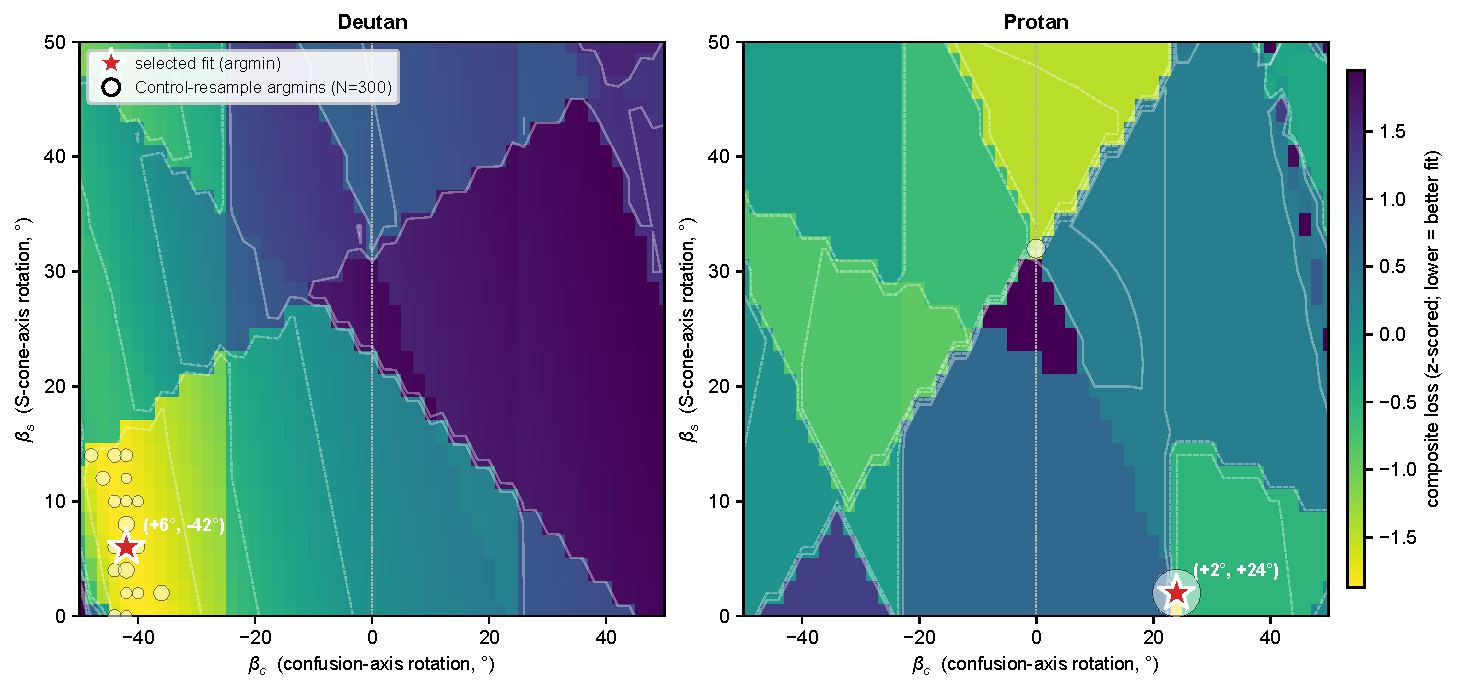
\includegraphics[width=\textwidth]{figS1_landscape}
  \caption{\textbf{Per-subject loss landscape and parameter uncertainty.}
  The $z$-scored composite loss over the $(\beta_s, \beta_c)$ grid, reconstructed on the full seven-control pool, with lower values in yellow.
  The loss combination is $\gamma_{\rm OY} + L_{\rm RDM}^{(V2)}$ for the deutan participant and $\gamma_{\rm all} + L_{\rm RDM}^{(V1)}$ for the protan participant.
  The red star marks the argmin of that surface, at $(\hat\beta_s, \hat\beta_c) = (6^\circ, -42^\circ)$ for the deutan participant and $(2^\circ, +24^\circ)$ for the protan participant.
  It is a descriptive low-dimensional embedding of the distortion rather than a physiological point estimate.
  White points give the per-resample argmins over $N = 300$ control 5-train/2-test resamples.}
  \label{fig:landscape}
\end{figure}


% --------------------------------------------------------------------------
% ==== S13  Stability of the selected fits ====
% --------------------------------------------------------------------------

\suppsection{Stability of the selected fits}{app:fit_stability}

\paragraph{Control leave-one-out magnitude anchor.}
Both CVD estimates fall inside the corresponding control range, so parameter magnitude alone is a descriptive anchor rather than a test of CVD-versus-control specificity. Each of the $n = 7$ control participants was refit as a pseudo-CVD case with the remaining control pool as reference, under that participant's own selected loss. The deutan combination is $\gamma_{\rm OY} + L_{\rm RDM}^{(V2)}$ and the protan combination $\gamma_{\rm all} + L_{\rm RDM}^{(V1)}$. The deutan estimate is $\|\hat\beta\| = 42.4^\circ$ against a control range of $30.5^\circ$ to $58.1^\circ$ (mean $49.1^\circ$). The protan estimate is $24.1^\circ$ against $23.4^\circ$ to $55.5^\circ$ (mean $35.7^\circ$), close to the lower bound.

\paragraph{Sign stability across the two preprocessing pipelines.}
Each participant's selected loss combination was refit on the head-motion-corrected pipeline (\cref{app:uncorrected}) with every other element of the procedure held fixed, and the two participants diverge. The sign of $\hat\beta_c$ held for the deutan participant, whose median moved from $-42^\circ$ to $-46^\circ$ with the fraction of negative resamples at $1.000$ and $0.947$. It reversed for the protan participant, whose median moved from $+24^\circ$ to $-12^\circ$, with the head-motion-corrected pipeline returning $79.3\%$ negative resamples against none under the primary pipeline. The deutan fit was also more poorly conditioned on the second pipeline, the combined fraction of resamples reaching a grid boundary rising from $0.09$ to $0.72$, and those boundary solutions lie on the same side as the median, so they bear on the magnitude rather than on the sign. The psychophysical atoms are independent of preprocessing, so the neural atom is the sole component that differs between the two fits. We therefore report the deployed protan parameter as a frozen value and give it no physiological interpretation.

\paragraph{Resample structure.}
Each participant's selected fit is the global minimum of its loss surface on the full data (\cref{fig:landscape}), and the $(32^\circ, 0^\circ)$ solution lies in the secondary basin of the protan PCA landscape, so the two reductions disagree about which basin is the minimum. Across the 300 resamples $\hat\beta_c$ concentrates at $-42^\circ$ and $-44^\circ$ ($202$ of $300$) and stays within $[-48^\circ, -36^\circ]$, whereas $\hat\beta_s$ is distributed almost uniformly from $0^\circ$ to $14^\circ$.

\paragraph{Gate statistics and neural-term ablation.}
Table~\ref{tab:fit_stability} collects the statistics that describe how each selected cell was reached and how stable it is. The separation block reports the precondition that admitted a $\Delta$RDM atom at a given ROI (\S\ref{sec:methods:selection}). The ablation block refits each participant's selected combination with the psychophysical atoms alone and with the $\Delta$RDM atom alone, holding every other element of the procedure fixed, so the three argmins are directly comparable. All entries are medians over the same $N = 300$ control 5-train/2-test resamples, on the PCA-basis loss unless the row names the SRM basis.

\begin{table}[htbp]
  \caption{Gate statistics, neural-term ablation, and resample stability for the two selected fits. Separation $d$ is the standardized distance between the participant and the control distribution at each ROI, and the $\Delta$RDM atom was admissible only where it was positive and exceeded the pre-set threshold (\S\ref{sec:methods:selection}), which left all four ROIs in the deutan participant and V1 alone in the protan participant. $\Delta\overline{L}$ is the change in an atom's held-out loss at the selected cell relative to the no-distortion cell $(0^\circ, 0^\circ)$, with negative values favoring the fitted distortion, and the fold count gives how many of the seven leave-one-out folds favor it. The boundary-saturation rate is the fraction of resamples whose solution reached a grid edge. Parameter IQRs are given as $(\beta_s, \beta_c)$.}
  \label{tab:fit_stability}
  \centering
  \small
  \begin{tabular}{lcc}
    \toprule
    & Deutan & Protan \\ \midrule
    \multicolumn{3}{l}{\emph{Separation precondition}} \\
    \quad $d$ at V1 / V2 / V3 / hV4 & $2.31$ / $1.94$ / $0.86$ / $2.19$ & $0.81$ / $-0.23$ / $-0.48$ / $-0.24$ \\
    \quad Loss combinations passing the gate & 25 & 4 \\ \midrule
    \multicolumn{3}{l}{\emph{Held-out generalization of the selected cell}} \\
    \quad Grid percentile & $4.6\%$ & $8.1\%$ \\
    \quad $\Delta\overline{L}$, psychophysical atom & $-13.85$ (5 of 7) & $+0.01$ (3 of 7) \\
    \quad $\Delta\overline{L}$, $\Delta$RDM atom & $-0.41$ (7 of 7) & $-0.47$ (7 of 7) \\ \midrule
    \multicolumn{3}{l}{\emph{Neural-term ablation (argmin)}} \\
    \quad Psychophysical atoms alone & $(16^\circ, -44^\circ)$ & $(26^\circ, +4^\circ)$ \\
    \quad $\Delta$RDM atom alone & $(4^\circ, -26^\circ)$ & $(0^\circ, +24^\circ)$ \\
    \quad Selected combination & $(6^\circ, -42^\circ)$ & $(2^\circ, +24^\circ)$ \\
    \quad Selected combination, SRM basis & $(8^\circ, -42^\circ)$ & $(32^\circ, 0^\circ)$ \\ \midrule
    \multicolumn{3}{l}{\emph{Resample stability, psychophysical alone $\rightarrow$ selected}} \\
    \quad Boundary-saturation rate & $0.23 \rightarrow 0.09$ & $0.00 \rightarrow 0.00$ \\
    \quad Parameter IQR, PCA basis & $(18^\circ, 6^\circ) \rightarrow (8^\circ, 2^\circ)$ & $(6^\circ, 4^\circ) \rightarrow (0^\circ, 0^\circ)$ \\
    \quad Parameter IQR, SRM basis & $(18^\circ, 6^\circ) \rightarrow (10^\circ, 4^\circ)$ & $(6^\circ, 4^\circ) \rightarrow (0^\circ, 2^\circ)$ \\
    \bottomrule
  \end{tabular}
\end{table}


\suppsection{Filter-evaluation session design and comparator}{app:filter_eval}

\paragraph{Comparator.}
The deployed comparator was the macOS accessibility Color Filter (System Settings $>$ Accessibility $>$ Display, build 26.5.1), set at an intensity the participant self-tuned before scanning. It is the unmodified shipping product, an operating-system-level post-display transform. We compared against it rather than a re-implemented retinal-simulation transform so that the comparator is the correction an end user actually encounters. The individualized filter was rendered directly in PsychoPy from the frozen per-subject pre-image.

\paragraph{Acquisition.}
Eight fMRI runs were acquired in ABBA-counterbalanced order, four per filter. Scanner time set this count, since six runs per condition would run roughly 90 minutes, beyond the 60--75-minute window over which participant attention and head motion stay acceptable. Four runs per condition take about 60 minutes, at the lower edge of that window.

\paragraph{Run-count adequacy.}
Four runs preserve the Session-1 separation between the control mean and the two CVD cases at hV4. Across all $\binom{6}{n}$ subsets of the six-run Session-1 data, hV4 LOCO adjacent accuracy held that separation at every run count down to four (\cref{fig:adjacc_saturation}). At $n = 4$ the control mean reached $0.45$ against $0.46$ at six runs and stayed above the $0.25$ chance level, while both CVD participants stayed below it (deutan $0.23$, protan $0.14$, single-case $d_{cc} < -2$ in both). Four runs nonetheless fall below the count recommended for fine-grained RDM-based model comparison, so the second session targets movement toward or away from the control reference rather than adjudication between model classes.

The filter conditions each have four runs, whereas the Session-1 control reference and the unfiltered baseline each have six. Noise in either pattern inflates disparity and RDM similarity, so an unmatched comparison would penalize the filter conditions twice, once against the baseline and once against the control distribution that the single-case test uses. Every neural index is therefore reported run-matched. For the interpolation indices the control reference is subsampled to four runs. For the geometry indices both the control means and the unfiltered baseline are rebuilt from four runs, exhaustively over all $\binom{6}{4} = 15$ subsets, with the shared response model refitted within each subset and the resulting metrics averaged (\texttt{exp2\_runmatched\_geometry.py}). The filter conditions themselves are never subsampled. The control reference comprises $n = 7$ controls at V1--V3 and $n = 6$ at hV4, where one control has too few voxels. Matching raises the protan V1 RDM similarity of the unfiltered baseline from $0.25$ to $0.33$, which places the individualized filter's value below that baseline rather than above it, and leaves the ordering of conditions unchanged on all four indices.
% TERMINOLOGY (resolved 2026-08-05): was "RDM-based model discrimination"; changed to
% "model comparison". "discrimination" is now reserved paper-wide for the behavioral
% JND construct; the neural LORO construct is "color classification".

\begin{figure}[tb]
  \renewcommand{\thefigure}{S\arabic{figure}}  % see the note on the first supplementary figure
  \centering
  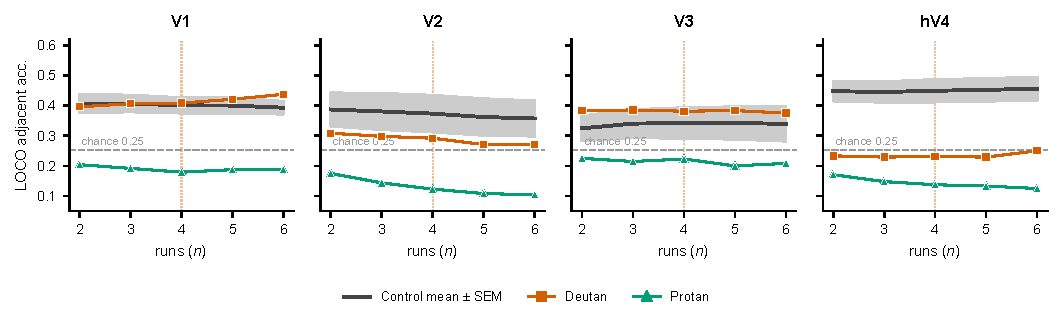
\includegraphics[width=\linewidth]{figS2_adjacc_saturation}
  \caption{\textbf{Hue-interpolation adjacent accuracy as a function of the number of runs.} LOCO adjacent accuracy (six-channel basis, OLS pseudoinverse decoder) as a function of the number of runs $n$, computed over all $\binom{6}{n}$ run subsets of the Session-1 data, per ROI. Black line, control mean $\pm$ SEM (shaded band); dashed line, the $0.25$ chance level; markers, the two CVD single cases (deutan, protan). The orange guide marks the deployed $n = 4$.}
  \label{fig:adjacc_saturation}
\end{figure}

\paragraph{Single-case inference.}
Each condition's neural index was compared to the control distribution as the case-control effect size $d_{cc}$ (\S\ref{sec:methods:stats}), reported in place of an inferential $p$ because the grand-mean permutation null is biased for this design. Robustness was assessed by leave-one-run separation, the contrast holding after any single run is dropped, and by re-extracting both conditions on the no-filter baseline voxel set.

% --------------------------------------------------------------------------
% ==== S15  Second-session outcomes by condition ====
% Split from the former "Filter-evaluation session design and comparator"
% on 2026-09-04: the design half and the condition-level results half each
% carry their own exhibits (words_trimming.md §5.4).
% --------------------------------------------------------------------------

\suppsection{Second-session outcomes by condition}{app:exp2_outcomes}

Each index below is reported for the unfiltered Session-1 baseline (NF), the deployed accessibility filter (Dep), and the individualized filter (Ind), run-matched as described in \cref{app:filter_eval}.

\paragraph{Hue identification (8AFC).}
Identification accuracy stayed at or above the Session-1 baseline under the individualized filter in both participants (\cref{tab:exp2_8afc}). This task entered neither fitting term, so it is a prospective test of the filters (\S\ref{sec:results:filter_eval}).

\begin{table}[tb]
  \centering
  \caption{\textbf{Second-session hue identification (8AFC).} Accuracy over $n = 64$ trials per cell with the 95\% Wilson score interval. Chance $= 0.125$. NF, no-filter (Session-1 baseline); Dep, deployed accessibility filter; Ind, individualized filter.}
  \label{tab:exp2_8afc}
  \begin{tabular}{llcc}
    \toprule
    Participant & Condition & Accuracy & 95\% CI \\
    \midrule
    Deutan & NF  & 0.81 & $[0.70, 0.89]$ \\
                    & Dep & 0.97 & $[0.89, 0.99]$ \\
                    & Ind & 0.97 & $[0.89, 0.99]$ \\
    \midrule
    Protan & NF  & 1.00 & $[0.94, 1.00]$ \\
                    & Dep & 0.86 & $[0.75, 0.92]$ \\
                    & Ind & 0.98 & $[0.92, 1.00]$ \\
    \bottomrule
  \end{tabular}
\end{table}

\paragraph{Hue classification (LORO).}
The displayed hues remained decodable under both filters (\cref{tab:exp2_loro}). Every cell stayed above the $0.125$ chance level. The lowest cell, $0.50$ at hV4 under the individualized filter in the deutan participant, lies below the control range of $0.71$ to $0.77$.

\begin{table}[tb]
  \centering
  \caption{\textbf{Second-session hue classification (LORO eight-way classification accuracy).} Chance $= 0.125$. NF, no-filter (Session-1 baseline); Dep, deployed accessibility filter; Ind, individualized filter. Controls, mean ($n = 7$).}
  \label{tab:exp2_loro}
  \begin{tabular}{lccccccc}
    \toprule
     & & \multicolumn{3}{c}{Deutan} & \multicolumn{3}{c}{Protan} \\
    \cmidrule(lr){3-5} \cmidrule(lr){6-8}
    ROI & Controls & NF & Dep & Ind & NF & Dep & Ind \\
    \midrule
    V1  & 0.71 & 0.79 & 0.84 & 0.72 & 0.79 & 0.91 & 0.66 \\
    V2  & 0.71 & 0.79 & 0.69 & 0.62 & 0.83 & 0.75 & 0.72 \\
    V3  & 0.77 & 0.67 & 0.78 & 0.69 & 0.81 & 1.00 & 0.69 \\
    hV4 & 0.75 & 0.73 & 0.88 & 0.50 & 0.71 & 0.84 & 0.69 \\
    \bottomrule
  \end{tabular}
\end{table}

\paragraph{Interpolation and geometry by condition.}
The three neural indices of the second session appear in \cref{tab:exp2_geometry} at each participant's target region, with the control reference and the single-case effect size for every condition.

\begin{table}[tb]
  \centering
  \caption{\textbf{Second-session interpolation and representational geometry.} All entries are run-matched (four runs per cell). NF, no-filter (Session-1 baseline); Dep, deployed accessibility filter; Ind, individualized filter. Parenthetical values are Crawford--Howell single-case effect sizes $d_{cc}$ against the control distribution. For adjacent accuracy the control entry is the mean $\pm$ SD over $n = 6$ controls at hV4 and the analytic chance level is $0.25$. For SRM disparity the control entry is the mean over $n = 7$ controls and lower values are more control-like. For RDM similarity the control entry is the leave-one-out self-consistency, a single value with no dispersion, so no effect size is defined and higher values are more control-like. The target region is the one at which each participant's Session-1 disparity was elevated, V2 for the deutan and V1 for the protan participant.}
  \label{tab:exp2_geometry}
  \small
  \begin{tabular}{lcccc}
    \toprule
    Index & Controls & NF & Dep & Ind \\
    \midrule
    \multicolumn{5}{l}{\emph{Deutan}} \\
    \quad hV4 adjacent accuracy & $0.46 \pm 0.11$ & $0.23$ ($-2.11$) & $0.25$ ($-1.94$) & $0.31$ ($-1.35$) \\
    \quad V2 SRM disparity & $0.44$ & $0.68$ ($2.69$) & $0.87$ ($4.93$) & $0.77$ ($3.73$) \\
    \quad V2 RDM similarity & $0.59$ & $0.42$ & $0.16$ & $0.05$ \\
    \midrule
    \multicolumn{5}{l}{\emph{Protan}} \\
    \quad hV4 adjacent accuracy & $0.46 \pm 0.11$ & $0.14$ ($-2.99$) & $0.19$ ($-2.52$) & $0.06$ ($-3.70$) \\
    \quad V1 SRM disparity & $0.43$ & $0.70$ ($3.92$) & $0.66$ ($3.29$) & $0.63$ ($2.84$) \\
    \quad V1 RDM similarity & $0.66$ & $0.33$ & $0.38$ & $0.26$ \\
    \bottomrule
  \end{tabular}
\end{table}

\paragraph{Forward-tuning encoding index.}
The forward-tuning correlation $\rho$ is the Pearson correlation between the predicted and the observed voxel pattern, averaged over the eight held-out hues. It indexes the encoding fit rather than the decoding accuracy on which the comparison rests. Figure~\ref{fig:forward_tuning} shows this index against the reference hue map, reported as corroboration only, since it lies outside the validated Session-1 decoding pipeline. In the deutan participant the individualized filter approaches the control level at hV4 ($\rho = +0.18$ against controls $+0.21$) while under the deployed filter it falls to $\rho = -0.39$. In the protan participant the three conditions do not separate, all reaching $\rho \approx -0.02$ at hV4.

\begin{figure}[tb]
  \renewcommand{\thefigure}{S\arabic{figure}}  % see note on the previous figure
  \centering
  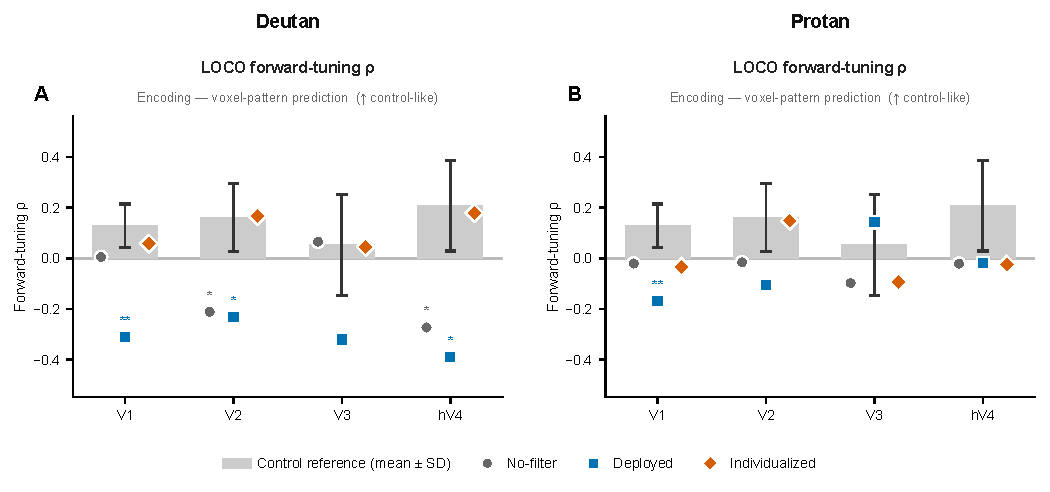
\includegraphics[width=\linewidth]{figS3_forward_tuning}
  \caption{\textbf{Forward-tuning encoding index (corroboration only).} LOCO forward-tuning correlation $\rho$ to the reference hue map across V1--hV4, for the deutan (left) and protan (right) participants ($\uparrow$ control-like). Gray bars, control reference (mean $\pm$ SD, $n = 7$); markers, no-filter (gray circle), deployed accessibility filter (blue square), individualized filter (orange diamond). Stars, Crawford--Howell single-case deviation from the control distribution ($^{*}p<.05$, $^{**}p<.01$).}
  \label{fig:forward_tuning}
\end{figure}


% ========== Section 14: Effect Sizes ==========

% --------------------------------------------------------------------------
% ==== S16  Statistical analysis and effect sizes ====
% Merger of the former "Effect sizes for single-case comparisons" and
% "Statistical analysis" sections (2026-09-04). The two defined d_cc in terms
% of each other; Methods §sec:methods:stats now points here once.
% The cross-subject encoder-transfer comparison moved to \cref{app:decoders},
% where it belongs with the decoder results (words_trimming.md §5.4).
% --------------------------------------------------------------------------

\suppsection{Statistical analysis and effect sizes}{app:statistics}

Unless noted otherwise, the significance threshold was $\alpha = 0.05$. False Discovery Rate correction \parencite{benjamini1995} was applied within two pre-specified families alone, the RDM hue-pair comparisons ($q = 0.05$, 28 pairs per participant) and the six parameter-identifiability checks (\cref{sec:methods:identifiability}). The exploratory per-hue vulnerability comparisons and the per-pair identification tests, including the blue-hue deficit, are reported one-tailed and uncorrected. Individual CVD participants were compared to the control distribution using the \textcite{crawford1998} modified $t$-test,

with the tail set by the pre-specified direction of each endpoint, one-tailed upper for disparity, one-tailed lower for interpolation, and two-tailed for classification and for the activation metrics.

Single-case effect sizes are the case-control index $d_{cc} = (x_{\rm case} - \bar{x}_{\rm ctrl}) / s_{\rm ctrl} = t\sqrt{(n+1)/n}$, where $n$ is the control sample size used in the test. Mann--Whitney $U$ tests use the rank-biserial correlation $r_{\rm rb}$ as their effect size, and group-level effect sizes are Hedges' $g$ \parencite{hedges1985}. Effect sizes for the single-case interpolation comparisons appear in \cref{tab:effect_sizes}, and the geometric-disparity effect sizes appear beside their $t$ statistics in \cref{tab:disparity_loso}. Single-case comparisons of within-subject LORO accuracy against the control distribution reached $|d_{cc}|$ between $0.25$ and $1.58$ across the eight participant-by-ROI tests, with all $p \geq 0.189$ (two-tailed). The largest deviation was the deutan participant at V3 ($d_{cc} = -1.58$), and at hV4 both participants gave $d_{cc} = -1.08$ ($p = 0.352$).

\begin{table}[h]
\centering
\caption{Effect sizes for the single-case hue-interpolation comparisons at hV4 (main text, \S\ref{sec:results:loco}). Crawford--Howell case-control effect size $d_{cc} = t\sqrt{(n+1)/n}$ against the $n = 7$ control distribution, one-tailed. Per-hue tests are uncorrected and exploratory across eight hues. Both CVD participants share identical statistics at the three hues where adjacent accuracy is zero. Blue lies just above the conventional threshold and is the largest per-hue deviation.}
\label{tab:effect_sizes}
\begin{tabular}{lccc}
\toprule
Comparison (hV4) & $t$ & $p$ & $d_{cc}$ \\
\midrule
LOCO adjacent accuracy, deutan & $-1.89$ & $0.054$ & $-2.02$ \\
LOCO adjacent accuracy, protan & $-3.04$ & $0.012$ & $-3.25$ \\
\midrule
\multicolumn{4}{l}{\emph{Per-hue adjacent accuracy (one-tailed, exploratory; both participants)}} \\
Blue & $-1.93$ & $0.051$ & $-2.06$ \\
Purple & $-0.79$ & $0.229$ & $-0.85$ \\
Magenta & $-1.47$ & $0.096$ & $-1.57$ \\
\bottomrule
\end{tabular}
\end{table}


\suppsection{Alignment robustness of the within-subject readouts}{app:alignment}

The two alignment spaces agree on the pattern on which the Results rest. LORO and LOCO are trained and tested within a single participant, so the main text computes them on the Procrustes-aligned amplitudes, which retain that participant's voxels at full resolution, and SRM enters only where a comparison spans participants. \cref{tab:alignment} gives both readouts in the Procrustes space, and the hue-channel-basis rows of \cref{tab:loro_decoders,tab:loco_decoders} give the same readouts in the SRM space.

Classification stays above the $0.125$ chance level for both CVD participants at every region in both spaces, with the lowest cell at $0.312$. Interpolation at hV4 remains reduced in both participants in both spaces, and the ordering of the two participants is preserved. Procrustes alignment yields the higher control-mean accuracy at all four regions for classification and at three of the four for interpolation, and it is the higher of the two spaces in 26 of the 36 participant-by-region classification cells. This follows from the dimensionality reduction in SRM discarding response variance that a within-subject readout can otherwise use.

The spaces differ at V1 classification, where SRM places both CVD participants above the control mean ($d_{cc} = +0.59$ and $+0.79$) while Procrustes places them slightly below ($d_{cc} = -0.25$ for both). Every single-case classification comparison stayed short of significance in both spaces.

\begin{table}[h]
\centering
\caption{Hue-channel basis readouts in the Procrustes-aligned space, which the main text reports. LORO is eight-way classification accuracy (chance $0.125$); LOCO is adjacent accuracy (analytic chance $0.25$). The control column is the mean over $n = 7$. The SRM-aligned counterpart of every cell appears in the forward-encoding rows of \cref{tab:loro_decoders,tab:loco_decoders}.}
\label{tab:alignment}
\begin{tabular}{lcccccc}
\toprule
& \multicolumn{3}{c}{LORO classification} & \multicolumn{3}{c}{LOCO interpolation} \\
\cmidrule(lr){2-4}\cmidrule(lr){5-7}
Region & Controls & deutan & protan & Controls & deutan & protan \\
\midrule
V1  & $0.580$ & $0.562$ & $0.562$ & $0.393$ & $0.437$ & $0.188$ \\
V2  & $0.607$ & $0.521$ & $0.562$ & $0.357$ & $0.271$ & $0.104$ \\
V3  & $0.574$ & $0.396$ & $0.458$ & $0.339$ & $0.375$ & $0.208$ \\
hV4 & $0.488$ & $0.375$ & $0.375$ & $0.456$ & $0.250$ & $0.125$ \\
\bottomrule
\end{tabular}
\end{table}


% --------------------------------------------------------------------------
% ==== S17  (was Supplementary/S18_geometry_validity.tex) ====
% --------------------------------------------------------------------------
% Supplementary S16 — Validity of the geometric comparison
% 2026-08-07
% Governing document: docs/PAPER/REVISION_PLAN_MOTION_GEOMETRY_2026-08-06.md §S18 (rule R5).
% Source numbers: analysis/phase2_SRM_across_between/results/RESULTS_GEOMETRY_VALIDITY_2026-08-05.md
%   §1 (control positive control), §2 (color specificity), §4 (cyclic shift)
% Raw outputs: analysis/future_phase1_sensitivity/results/{with_residuals,hmc_v2}/color_correspondence/frozen_permutation.json,
%   analysis/validation/results/cyclic_shift_disparity.json (hmc_v2 variant not yet computed)
% Counts and BH-FDR recomputed from the JSON on 2026-08-07:
%   35 cells, 16 raw p<.05 (the "15" in RESULTS_GEOMETRY_VALIDITY §2 prose is a
%   miscount of its own table), 7 surviving BH; motion-regressed 18 raw / 15 BH.
% The cyclic-shift gain is referred to the control gain distribution, which is computed
%   under the same minimum-over-eight rule and therefore absorbs the same selection
%   bias. hV4 shift gains are omitted: the ROI carries no geometric endpoint, and
%   the motion-regressed control gain SD there collapses to 0.38%.

\suppsection{Validity of the geometric comparison}{app:geometry_validity}

The color-correspondence permutation has power only when the shared projection is held fixed, since re-estimating it at each permutation allows the re-fit to absorb the permutation. The permutation asks whether a participant's colors map onto the control geometry in the identity order, which differs from the color-label permutation null of the main text, where the question is whether the control group interpolates above chance in a region. We tested both variants on the controls, in whom color structure is established. Re-estimation detected 0 of 7 at V1, V2 and V3 and 0 of 6 at hV4, with mean permutation $z$ near zero in every ROI, whereas freezing the projection recovered detection, reaching 5 of 7 at V3 and 2 to 3 of 7 elsewhere (\cref{tab:frozen_control}). Every color-specificity result below uses the frozen projection.

\begin{table}[h]
\centering
\caption{Color-correspondence permutation on the controls, used as a positive control. Detection counts and mean permutation $z$ under a projection re-estimated at each permutation and under a frozen projection. Lower $z$ indicates a better identity correspondence than the shuffled null.}
\label{tab:frozen_control}
\begin{tabular}{lccccc}
\toprule
 & & \multicolumn{2}{c}{Re-estimated} & \multicolumn{2}{c}{Frozen} \\
\cmidrule(lr){3-4}\cmidrule(lr){5-6}
ROI & $n$ & detected & mean $z$ & detected & mean $z$ \\
\midrule
V1  & 7 & 0 & $-0.04$ & 2 & $-1.58$ \\
V2  & 7 & 0 & $-0.04$ & 3 & $-1.00$ \\
V3  & 7 & 0 & $-0.78$ & 5 & $-2.39$ \\
hV4 & 6 & 0 & $+0.06$ & 2 & $-1.07$ \\
\bottomrule
\end{tabular}
\end{table}

Both CVD participants showed color-specific geometry. The deutan participant reached $p = .002$ at V2, the lowest V2 value among the nine participants, and $p = .024$ at V3. The protan participant reached $p = .001$ at V3 and $p = .013$ at V2, while V1 returned $p = .758$. Across the 35 participant-by-ROI cells, 16 fell below $.05$ against a chance expectation of $1.8$, and 7 survived Benjamini--Hochberg correction over all 35 (\cref{tab:color_specificity}). Two of the survivors belong to the CVD participants, the deutan V2 cell ($q = .018$) and the protan V3 cell ($q = .012$). V3 showed color specificity most broadly, with 5 of its 9 cells surviving.

\begin{table}[h]
\centering
\caption{Color-correspondence permutation under the frozen projection, one cell per participant and region, in the two preprocessing pipelines. Entries give $p_{\rm perm}$ against $N = 1{,}000$ permutations. Seven cells survive Benjamini--Hochberg correction across the 35 cells of the primary pipeline and none survive it in the head-motion-corrected pipeline.}
\label{tab:color_specificity}
\begin{tabular}{lcccccccc}
\toprule
 & \multicolumn{4}{c}{Primary} & \multicolumn{4}{c}{Head-motion correction} \\
\cmidrule(lr){2-5}\cmidrule(lr){6-9}
Participant & V1 & V2 & V3 & hV4 & V1 & V2 & V3 & hV4 \\
\midrule
Control 1 & $0.088$ & $0.020$ & $0.062$ & $0.393$ & $0.012$ & $0.072$ & $0.018$ & $0.290$ \\
Control 2 & $0.001$ & $0.016$ & $0.004$ & $0.136$ & $0.437$ & $0.420$ & $0.191$ & $0.019$ \\
Control 3 & $0.109$ & $0.520$ & $0.255$ & $0.272$ & $0.325$ & $0.113$ & $0.176$ & $0.101$ \\
Control 4 & $0.152$ & $0.014$ & $0.001$ & $0.041$ & $0.420$ & $0.006$ & $0.015$ & $0.173$ \\
Control 5 & $0.057$ & $0.773$ & $0.034$ & $0.031$ & $0.079$ & $0.194$ & $0.032$ & $0.038$ \\
Control 6 & $0.407$ & $0.290$ & $0.009$ & $0.220$ & $0.373$ & $0.117$ & $0.010$ & $0.012$ \\
Control 7 & $0.034$ & $0.159$ & $0.004$ & --- & $0.008$ & $0.005$ & $0.391$ & --- \\
\textbf{Deutan} & $0.105$ & $0.002$ & $0.024$ & $0.273$ & $0.022$ & $0.003$ & $0.047$ & $0.257$ \\
\textbf{Protan} & $0.758$ & $0.013$ & $0.001$ & $0.129$ & $0.010$ & $0.148$ & $0.053$ & $0.815$ \\
\bottomrule
\end{tabular}
\end{table}

Under head-motion correction 15 cells fell below $.05$ and none survived correction. The deutan V2 cell remained at its nominal value across the two pipelines ($p = .002$ and $p = .003$) while its corrected value moved from $q = .018$ to $q = .053$, and the protan V1 cell moved from $p = .758$ to $p = .010$. Individual cells of this grid are descriptive and support no claim in the main text.

The protan participant's V1 correspondence is displaced by one hue step, and the failure is not one of signal. That participant's V1 split-half pattern reliability reaches $.847$, above the highest control value, and eight-way classification there reaches $0.79$ against a chance level of $0.125$. Rotating the color labels by $45^\circ$ lowered Procrustes disparity from $1.037$ to $0.788$, a gain of $24.0\%$. We referred that gain to the distribution of shift gains across the seven controls ($3.5 \pm 5.9\%$), which is computed under the same minimum-over-eight rule and is therefore subject to the same selection bias. The protan gain exceeded that distribution (Crawford--Howell $t = 3.22$, $p = .009$, $d_{cc} = 3.44$), and the rotated geometry sat below the control mean disparity of $0.839 \pm 0.087$. The same rotation raised the second-order RSA similarity from $\rho \approx 0.00$ to $\rho = +0.52$, against a control mean of $0.45$, exceeding its own selection-bias null ($z = +5.02$, $p = .002$, $p_{\rm adj} = .032$). Disparity at this region is nonetheless elevated in both pipelines, so the departure is not accounted for by a rigid relabeling alone. The account applies to the primary pipeline, since that cell is no longer null under head-motion correction. The deutan participant showed the identity mapping as optimal at V1, V2 and V3.

Which rearrangement restores control-level similarity remains open. Under the SRM basis a $225^\circ$ shift ($+0.50$) is close to the $315^\circ$ optimum ($+0.52$). Under the PCA basis the optimum falls at $135^\circ$ ($p = .048$, which does not survive correction).

\end{document}
%:
